% !TeX program = xelatex
\documentclass[UTF8,11pt,a4paper]{ctexart}

% Common packages
\usepackage[margin=2.5cm]{geometry}
\usepackage{amsmath,amssymb}
\usepackage{graphicx}
\graphicspath{{assets/}}
\usepackage{booktabs}
\usepackage{enumitem}
\usepackage{titlesec}
\usepackage[hidelinks]{hyperref}
\usepackage{subcaption}

% Paragraph formatting: no first-line indent, with a small gap between paragraphs
\setlength{\parindent}{0pt}
\setlength{\parskip}{0.5em plus 0.1em minus 0.1em}
\setlist{itemsep=0pt,parsep=0pt}

% Display paragraph headings on their own line instead of as run-in headings
\titleformat{\paragraph}[block]
  {\normalfont\normalsize\bfseries}{\theparagraph}{1em}{}
\titlespacing*{\paragraph}{0pt}{1.5ex plus 0.2ex minus 0.2ex}{0.5em}

% English names for floats and headings (ctex defaults to Chinese)
\renewcommand{\figurename}{图}
\renewcommand{\tablename}{表}
\renewcommand{\contentsname}{目录}
\numberwithin{figure}{section}

% Document information
\title{%
  {\Huge 工业4.0}\\[0.4em]
  {\Large Industrie 4.0 für Ingenieure}\\[0.8em]
  {\small 课程总结}%
}
\author{作者：楼骁}

\begin{document}

\pagenumbering{gobble}
\maketitle
\clearpage
\tableofcontents
\clearpage
\pagenumbering{arabic}

% Main content starts here (each major section starts on a new page)
\let\oldsection\section
\renewcommand{\section}{\clearpage\oldsection}

\section{课程简介}

这门课是由 MHI，即 Gemeinschaftsvorlesung der Wissenschaftlichen Gesellschaft Montage, Handhabung und Industrierobotik 组织的联合课程。MHI 是由德语区多所大学的教授组成的学术网络，主要研究方向包括装配技术、搬运技术和工业机器人。

后续课程会涉及软件与控制技术、工业机器人、人机交互、传感系统、定位与基于位置的服务、工业数据科学、机器学习与人工智能、仿真与编程技术、工业 4.0 的标准和参考架构，以及增材制造中的数字化等内容。

\subsection{工业4.0的概念}

工业发展的历史通常被划分为\emph{四次工业革命}：
\begin{itemize}
    \item 工业 1.0 指的是以水力和\emph{蒸汽机}为基础的机械化生产。
    \item 工业 2.0 指的是以电力和\emph{流水线}为基础的大规模生产
    \item 工业 3.0 指的是通过电子技术、\emph{信息技术和计算机}实现的自动化生产
    \item 工业 4.0 则指当前阶段的\emph{网络化}、数据化和智能化生产
\end{itemize}

因此，工业 4.0 并不只是“工厂里使用机器人”这么简单。它的核心在于将机器、产品、传感器、软件系统、数据平台和人连接起来，使生产系统能够采集数据、交换信息、分析状态，并在此基础上优化生产过程。工业 4.0 的目标是让生产系统更加灵活、透明、高效，并能够适应更复杂和更个性化的生产需求。

在工业 4.0 中，一个重要概念是\emph{信息物理系统，也就是 Cyber-Physical Systems，简称 CPS}。它指的是物理设备和数字系统高度耦合的系统。例如，一台现代机床不仅仅是机械设备，它还可以通过传感器采集运行数据，通过控制器和网络接口传输数据，并利用软件系统对状态进行监测、分析和优化。这样，现实中的物理过程和数字世界中的信息处理就被连接在一起。

另一个关键概念是 RAMI 4.0，即“工业 4.0 参考架构模型”。它可以理解为描述工业 4.0 系统的三维坐标系。这个模型从三个维度来组织工业 4.0 系统：
\begin{itemize}
    \item 从物理资产到业务层面的不同层级。
    \item 产品或设备从开发、生产、使用到维护的生命周期。
    \item 从单个产品、现场设备、控制设备、工作站、企业到互联世界的层级结构。
\end{itemize}

RAMI 4.0 的作用是帮助人们系统化地理解复杂的工业 4.0 系统。它强调，工业 4.0 不能只从单一技术角度理解，比如只看机器人、传感器或云平台。真正的工业 4.0 涉及物理设备、通信、数据、功能、业务流程、产品生命周期和企业层级之间的整体集成。

工业 4.0 不只是技术问题。除了物联网、人工智能、机器人、云计算和大数据等技术之外，它还涉及开放标准、数字世界与现实世界的集成、网络基础设施、安全、工作组织、教育培训、法律框架和资源效率等问题。

\subsection{物联网 IoT}

IoT 的本质就是让物理世界中的物体具备感知、通信、计算和行动能力，从而与数字世界形成闭环。下面这七点分别对应实现这个闭环所必需的技术前提。
\begin{enumerate}
    \item 泛在通信（Uniquitäre Kommunikation）：物联网设备数量级远超传统互联网终端，而且很多分布在极其分散、甚至难以人工触达的位置。这就要求通信不再局限于Wi-Fi/以太网，而要覆盖低功耗广域网、蜂窝网络、短距无线等多种技术组合，做到随时随地都能连上。
    \item 大数据与云计算（Big Data and Cloud Computing）：海量设备持续产生数据流，单个终端的算力和存储不足以处理。云计算提供弹性的存储与计算资源，大数据技术则负责从这些高维、高频、异构的数据中提取有用信息。
    \item 整体环境感知（Holistische Umwelterfassung）：单一传感器只能提供局部、片面的信息。整体强调的是多模态传感器融合，加上多点位覆盖，才能重建一个足够完整、可用于决策的环境模型。
    \item 所有实体的移动性（Mobilität aller Entitäten）：IoT中的物往往不是静止的。这要求网络架构支持无缝切换、位置感知以及移动场景下的服务连续性。
    \item 能量自主（Hierachiefreie Energieautonomie）：很多IoT节点部署在无法接入电网、也难以频繁更换电池的地方。因此需要不依赖固定基础设施的供能方式，能灵活转换多种能量来源为电能的能量采集技术。这一点直接决定了IoT系统能否实现真正的部署后免维护。
\end{enumerate}
这五点合在一起，构成了从物理感知，到网络传输，再到智能决策的完整技术链条，这也是为什么它们被称为IoT的使能者，而不只是组成部分。少了任一环，系统要么无法规模化部署，要么无法真正自主运行。


\section{工业 4.0 中的控制技术}

\subsection{控制技术方式}

在传统工厂中，机器主要依赖固定硬件和本地控制。例如一台 CNC 机床、一台机器人、一套 PLC 控制柜，各自完成自己的任务。而工业 4.0 的核心趋势是把这些设备联网、数字化、软件化，使它们能够交换数据、被监控、被优化，甚至在一定程度上自主调整。

我们用 Software Defined Manufacturing (SDM) 来描述这个趋势：工业自动化正在从 hardware-oriented 转向 software-oriented。也就是说，以前重点是专用硬件和固定功能；未来重点是软件模块、虚拟化、云技术、数字孪生、AI 和自适应系统。

\subsection{工业控制系统的类型}

我们把常见控制系统分成 NC、RC、MC、SPS 和 MES。

工厂不是一个单一控制器控制所有东西，而是按层级组织的。越靠近现场设备，越强调实时性；越靠近管理层，越强调计划、调度、数据和业务流程。控制层级从 E1 到 E7：
\begin{itemize}
    \item E1 是过程层，例如传感器和执行器
    \item E2 是单机控制
    \item E3 是机器控制
    \item E4 是单元/工作站层
    \item E5 是生产线或车间管理层
    \item E6 是计划层
    \item E7 是工厂控制层
\end{itemize}

越往下，越接近物理过程，实时性要求越高。

NC 是 Numerical Control，数控，典型对象是 CNC 机床。它的任务是根据数字程序控制刀具或工件的运动。例如铣削、车削、钻孔时，程序给出几何路径、进给速度、主轴转速等，NC 将这些信息转换成各个轴的运动命令。NC 的特点包括：
\begin{itemize}
    \item 通过数字进行控制
    \item 按 DIN 66025 编程
    \item 处理多个自由度
    \item 将笛卡尔坐标转换为轴坐标
\end{itemize}

NC 常用于工具机、模具加工和机械制造，并追求高绝对精度。

RC 是 Robot Control，机器人控制。它控制的是工业机器人，特别是串联机械臂。机器人控制的重点不是切削路径，而是末端执行器或夹爪的空间运动。机器人程序可以通过离线编程、Teach-In 或 Playback 得到。它需要在关节坐标和空间坐标之间做坐标变换。

RC 常用于汽车制造、装配和搬运，重点通常是高重复精度，而不一定是像 CNC 那样的高绝对精度。

MC 是 Motion Control，运动控制。它关注多个轴之间的同步运动，例如印刷机、包装机、飞锯、输送带同步、电子凸轮等。它的核心不是“走一条复杂加工轨迹”，而是让多个驱动轴按照严格时序协同运动。比如一条高速包装线中，输送带、切刀、推料机构必须在毫秒级时间内协调，否则产品会错位。

SPS 是 Speicherprogrammierbare Steuerung，也就是 PLC。它是自动化中最基础、最常见的控制器。PLC 读取传感器输入，执行逻辑程序，然后控制阀门、电机、继电器、气缸等执行器。

SPS 按 DIN EN 61131-3 编程，处理模拟和数字信号，采用循环程序执行，直接连接传感器和执行器，并且结构紧凑、鲁棒。它广泛用于制造技术、过程工业和建筑自动化。

MES 是 Manufacturing Execution System，制造执行系统。它的位置高于机器控制，低于企业资源计划系统。MES 不直接以毫秒级控制电机，而是管理生产执行过程。例如订单执行、工位占用、生产状态、物料流、仓储、质量保证、数据采集、追溯和序列化。可以把 MES 理解为“车间层面的操作系统”：它知道哪个产品在什么工位、完成了什么步骤、用了什么材料、是否合格、下一步该去哪里。

图 \ref{fig:steuerungebene} 展示了这7个层级以及对应的功能。

\begin{figure}[htbp]
  \centering
  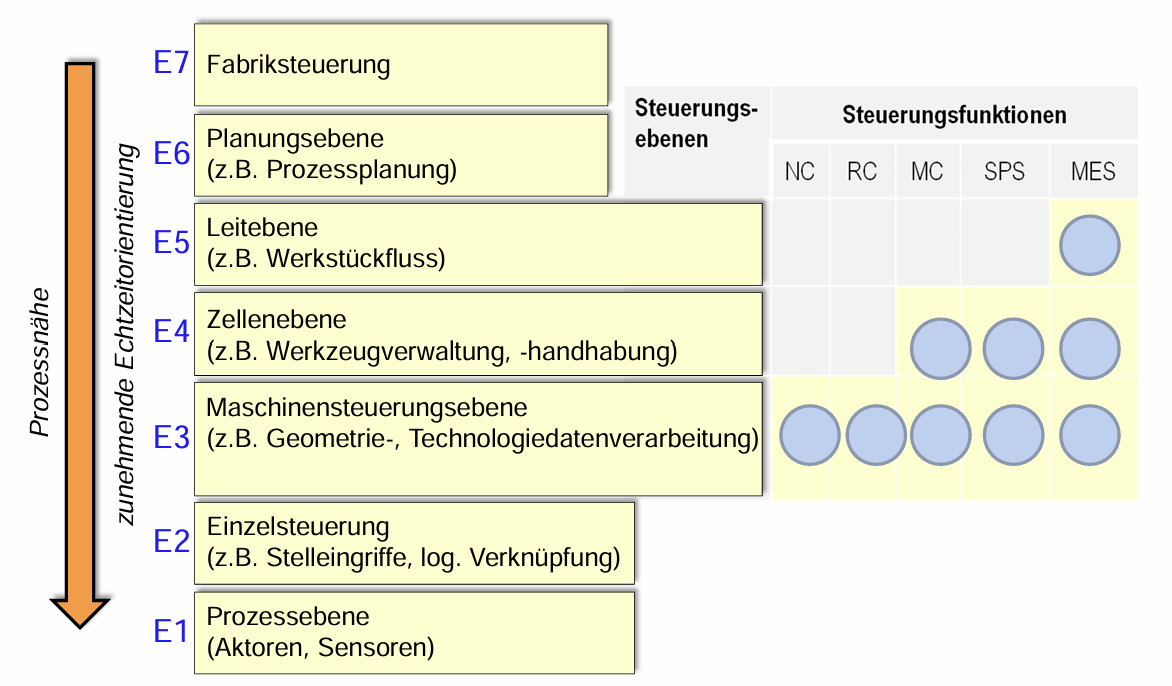
\includegraphics[width=0.8\textwidth]{steuerungebene.png}
  \caption{工厂的控制层级}
  \label{fig:steuerungebene}
\end{figure}

\subsection{控制架构}

我们不能只讲“有哪些控制器”，还要讲控制功能放在哪里。一个自动化系统通常有人机界面 HMI、逻辑控制和运动控制三类软件功能。我们用 OMAC 分类，把控制架构分成 PC-based、controller-based、drive-based 和 cloud-based。
\begin{itemize}
    \item PC-based 架构把 HMI、逻辑和运动控制集中在一台工业 PC 上。优点是软件集中、计算能力强、易于扩展和集成；缺点是实时性、可靠性和系统隔离必须通过合适的实时机制来保证。
    \item Controller-based 架构把逻辑和运动控制放在专用控制器中，HMI 则可能运行在单独的面板或 PC 上。这是工业中很常见、很稳健的架构。专用控制器更接近传统 PLC/CNC 控制方式，实时性和可靠性通常更容易保证。
    \item Drive-based 架构把一部分逻辑和运动控制下放到驱动器中。例如某些智能伺服驱动器不仅执行电流环、速度环，还能执行局部运动逻辑。这样可以减少上位控制器负担，提高局部响应速度。
    \item Cloud-based 架构则把部分功能放到边缘云或云端。它适合监控、优化、数据分析、预测性维护等任务，但不适合把严格毫秒级闭环控制完全放到远端云端，因为网络延迟和确定性难以保证。
\end{itemize}

\subsection{NC内部的信息流}

数控系统内部如何从加工任务变成实际轴运动。加工程序首先描述几何轮廓和工艺参数；控制系统解析程序；然后进行轨迹规划、插补、坐标变换；再生成每个轴的设定值；最后驱动器和伺服系统控制电机运动。这里的关键概念是“从抽象几何任务到实时轴控制”的转换。比如程序里写的是刀具从 A 点走到 B 点，但机器真正执行时，需要每个采样周期给 X、Y、Z 轴分别发送位置或速度指令。

\subsection{工业通信技术}
\label{subsec:industrialcommunication}

工业 4.0 不只是机器能动起来，还要求机器之间、机器与上位系统之间能够可靠交换数据。因此就得用到 ISO/OSI 七层模型，并把它和工业通信联系起来。

七层包括：
\begin{enumerate}
    \item 物理层
    \item 数据链路层
    \item 网络层
    \item 传输层
    \item 会话层
    \item 表示层
    \item 应用层
\end{enumerate}

例如：Ethernet、TSN 属于较底层的数据链路相关技术；IP 位于网络层；TCP/UDP 位于传输层；OPC-UA 属于应用层。

OPC-UA 可以理解为工业系统之间交换数据的标准语言。它解决的问题是：不同厂家、不同控制器、不同软件系统之间如何以统一方式描述和访问数据。例如一个控制器中的轴位置、温度、报警状态、设备 ID，如果没有统一语义，每个厂家都用自己的格式，系统集成会非常困难。OPC-UA 提供统一的信息模型和通信机制，使设备数据可以被上位系统、MES、SCADA 或其他应用读取和订阅。

TSN 是 Time Sensitive Networking，时间敏感网络。它的目标是让普通以太网具备确定性通信能力。普通以太网适合传文件、网页、邮件，但不能保证某个控制数据包一定在严格时间窗口内到达。工业控制尤其是运动控制需要确定性延迟、低抖动和同步。TSN 通过时间同步、优先级、带宽预留和时间窗口等机制，使工业网络更适合实时控制。课件用 OPC-UA PubSub over TSN 举例说明：应用层通过 OPC-UA 发布/订阅数据，底层通过 TSN 保证网络传输的时间确定性。

\subsection{实时操作系统}

实时系统的重点不是“速度快”，而是“在规定时间内可靠完成”。一个控制任务如果必须每 1 ms 更新一次轴位置，那么它不是平均 0.5 ms 完成就够了，而是每一次都必须在 deadline 之前完成。课件的学习检查问题中特别提到：进程调度状态、preemptive 与 non-preemptive scheduling、实时的含义，以及中断处理的时间行为。

Preemptive scheduling 是抢占式调度。高优先级任务到来时，可以打断低优先级任务。这适合实时控制，因为紧急任务可以及时执行。Non-preemptive scheduling 是非抢占式调度，一个任务开始后通常要运行到主动让出 CPU，这种方式简单，但对严格实时任务不利。中断处理也很重要，因为传感器、通信接口、驱动器反馈等事件可能需要立即响应。实时操作系统要保证中断延迟、任务切换延迟和周期任务执行时间可预测。
% !TeX root = main.tex
\section{工业机器人I}

\subsection{机器人结构与运动学}

\paragraph{机器人的分类}

在工厂里，我们经常需要设备把零件抓起来、移动、放下，这类设备统称为操作设备（Handhabungsgeräte）。它们大致分三种：
\begin{itemize}
    \item 靠人手动操作或远程遥控的装置
    \item 固定程序运动的装置
    \item 自由可编程运动的装置
\end{itemize}
工业机器人是一种自动控制的、可重复编程的多用途操作机，可在三个或三个以上轴上编程，既可固定安装，也可移动使用，用于工业自动化应用。属于自由可编程运动的装置。

工业机器人本身还可以按其程序自主性的高低做进一步细分，这关注的是机器人在运行过程中能在多大程度上自己做主：
\begin{itemize}
    \item \textbf{无自主程序影响（ohne selbsttätige Programmbeeinflussung）}：机器人按照固定程序执行。
    \item \textbf{有自主程序选择（mit selbsttätiger Programmselektion）}：机器人事先存有多套可选程序，运行时能够自己判断该调用哪一套程序。
    \item \textbf{有自主程序适应（mit selbsttätiger Programmadaption）}：机器人能根据实时感知到的环境或工件状态，对程序本身的参数甚至逻辑做出动态调整。
\end{itemize}

\paragraph{工业机器人的结构}

工业机器人可以看作由多个刚性连杆和关节组成的运动链。连杆（Glied）是机器人中近似刚性的构件。关节（Gelenk）连接两个连杆并允许它们产生相对运动的。轴（Achse）是指机器人中被驱动和控制的运动轴。关节的运动主要分为转动和平移。多个关节和连杆依次连接，构成了机器人的运动链。

自由度（Freiheitsgrad）表示一个机械系统能够独立运动的参数数量。关节数量不一定等于自由度数量。因为不同关节产生的运动可能存在约束，并非每一个关节都提供一个独立自由度。

\paragraph{坐标变换}

机器人系统中会同时存在多个坐标系，同一个点在不同坐标系中的坐标不同，因此需要通过\textbf{坐标变换}建立他们之间的关系。

假设有两个坐标系 \(A\) 和 \(B\)。如果 \(B\) 相对于 \(A\) 只是移动了，没有旋转，那么一个点从 \(B\) 坐标系转换到 \(A\) 坐标系时，只需要加上两个坐标系原点之间的位移：
\begin{equation}
    {}^A\mathbf p={}^B\mathbf p+{}^A\mathbf t_B
\end{equation}

但现实中 \(B\) 往往还相对于 \(A\) 发生了旋转。因此首先需要用旋转矩阵 \({}^A R_B\) 把向量的方向从 \(B\) 的坐标轴转换成 \(A\) 的坐标轴：

\begin{equation}
    \label{eq:rotationtranslation}
    {}^A\mathbf p={}^A R_B\,{}^B\mathbf p+{}^A\mathbf t_B
\end{equation}

这里 ${}^A R_B$ 表示“坐标系 \(B\) 相对于坐标系 \(A\) 的方向关系”，而 ${}^A\mathbf t_B$ 表示“\(B\) 的原点在 \(A\) 中的位置”。可以记成：下标是从哪里来，上标是到哪里去。

但是表达式 \ref{eq:rotationtranslation} 还是有一点麻烦，因为旋转是乘矩阵，平移却是加向量。为了让旋转和平移能够统一用一次矩阵乘法完成，我们引入第四个齐次坐标，把三维点 \((x,y,z)^T\) 写成 \((x,y,z,1)^T\)。然后定义齐次变换矩阵为
\begin{equation}
    {}^A T_B=
    \begin{bmatrix}
        {}^A R_B & {}^A\mathbf t_B\\
        0&0&0&1
    \end{bmatrix}
\end{equation}

这样表达式 \ref{eq:rotationtranslation} 就可以写成
\begin{equation}
    \begin{bmatrix}
        {}^A\mathbf p\\
        1
    \end{bmatrix}
    ={}^A T_B
    \begin{bmatrix}
        {}^B\mathbf p\\
        1
    \end{bmatrix}
\end{equation}

这就是齐次变换的意义：用一个矩阵同时表示两个坐标系之间的旋转和平移。

\paragraph{示例：坐标变换}

图 \ref{fig:roboterundwelt} 展示了一个机器人在操控一个物体。这个场景有4个坐标系，分别是世界坐标系W、机器人的基座坐标系B、机器人末端坐标系TCP、以及物体坐标系O。图中已知三个变换 \({}^W T_B\)、\({}^B T_{TCP}\)、和\({}^W T_O\)；两个未知变换 \({}^W T_{TCP}\) 和 \({}^{TCP}T_O\)。首先我们要明确：\({}^W T_B\) 表示 \(B\to W\)。接下来我们要来求这两个未知变换。

\begin{figure}[htbp]
  \centering
  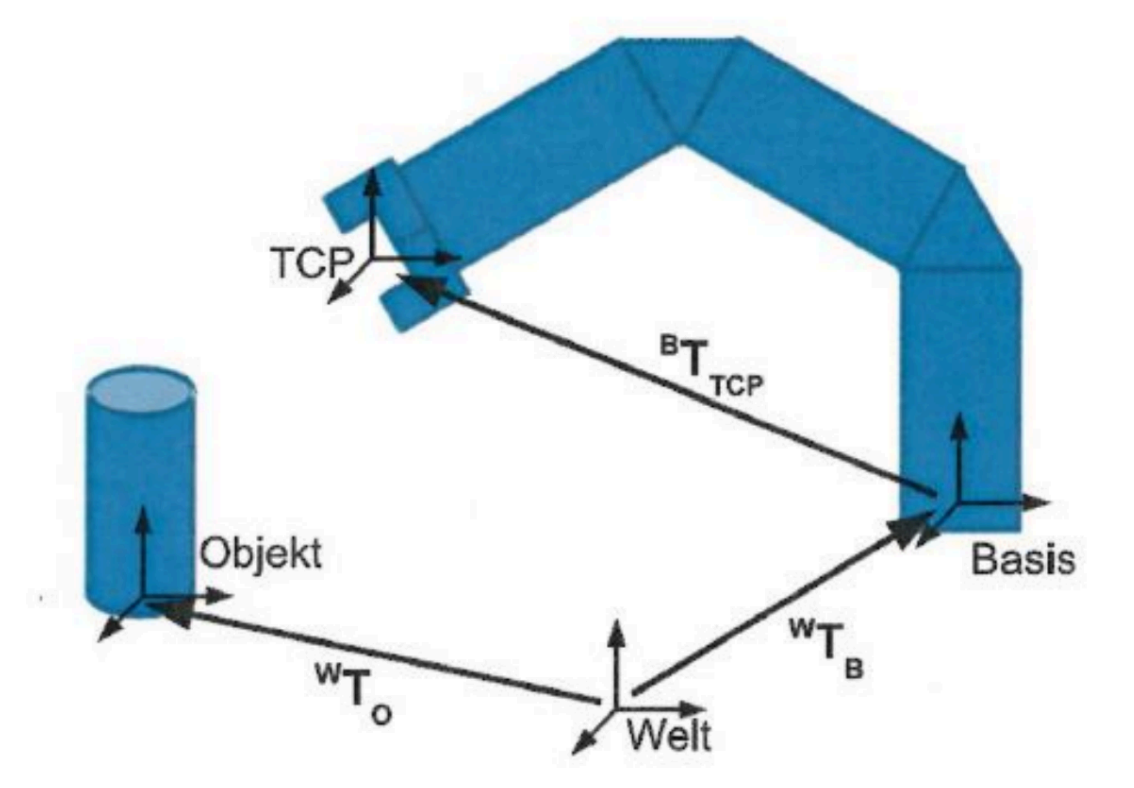
\includegraphics[width=0.5\textwidth]{roboterundwelt.png}
  \caption{一个机器人在环境中操控一个物体，它们有各自的坐标。}
  \label{fig:roboterundwelt}
\end{figure}

我们使用坐标变换的串联将 \(TCP\to B\) 和 \(B\to W\) 连接起来，自然就得到了 \(TCP\to B\to W\)。对应的矩阵就是 \({}^W T_B\,{}^B T_{TCP}\)。因此
\begin{equation}
{}^W T_{TCP}={}^W T_B\,{}^B T_{TCP}
\end{equation}
接下来我们求 \({}^{TCP}T_O\)。我们已知\({}^W T_O\)，也就是\(O\rightarrow W\)。但目标不是世界坐标系，而是 TCP，因此还需要：\(W\rightarrow TCP\)。问题在于我们前面得到的是 \(TCP\rightarrow W\)。方向反了，必须取逆：\({}^{TCP}T_W=({}^W T_{TCP})^{-1}\)。因此完整路径 \(O\rightarrow W\rightarrow TCP\) 的表达式为
\begin{equation}
    {}^{TCP}T_O=({}^W T_{TCP})^{-1}\,{}^W T_O=\left({}^W T_B\,{}^B T_{TCP}\right)^{-1}{}^W T_O
\end{equation}


\subsection{特性参数}

特性参数（Kenngrößen）描述这台机器人到底能不能完成某项任务，分为4大类：
\begin{itemize}
    \item \textbf{几何参数}描述的是机器人的尺寸以及它能够覆盖的空间。
    \item \textbf{负载参数}描述的是机器人的负载。
    \item \textbf{精度参数}描述的是机器人操作的精度。包括定位精度和重复精度。
    \item \textbf{运动参数}描述的是例如循环时间（完成一套动作需要的时间）、速度、加速度、稳定时间等参数。
\end{itemize}
这四个参数共同描述了机器人的性能。

\subsection{末端执行器与安全技术}

决定机器人能干什么任务的是装在机械臂末端的\textbf{末端执行器（Endeffektor）}。

\paragraph{夹爪是怎么抓住零件的}

夹爪要把一个零件稳稳固定住，靠的无非是三种抓力原理。
\begin{itemize}
    \item \textbf{力锁合（Kraftschluss）}：靠某种持续作用的力把物体夹紧，比如靠摩擦力、负压或磁力。
    \item \textbf{形锁合（Formschluss）}：靠零件和夹具的形状互相咬合。
    \item \textbf{质锁合（Stoffschluss）}：靠物质本身的状态变化把物体粘住，比如冷冻。
\end{itemize}

这三种夹爪形态的示例如图 \ref{fig:halterprinzipien} 所示。力锁合最常见也最灵活，形锁合精度高但夹具要专门定制，质锁合则多用于特殊工艺（比如玻璃、易碎品的临时固定）。

\begin{figure}[htbp]
  \centering
  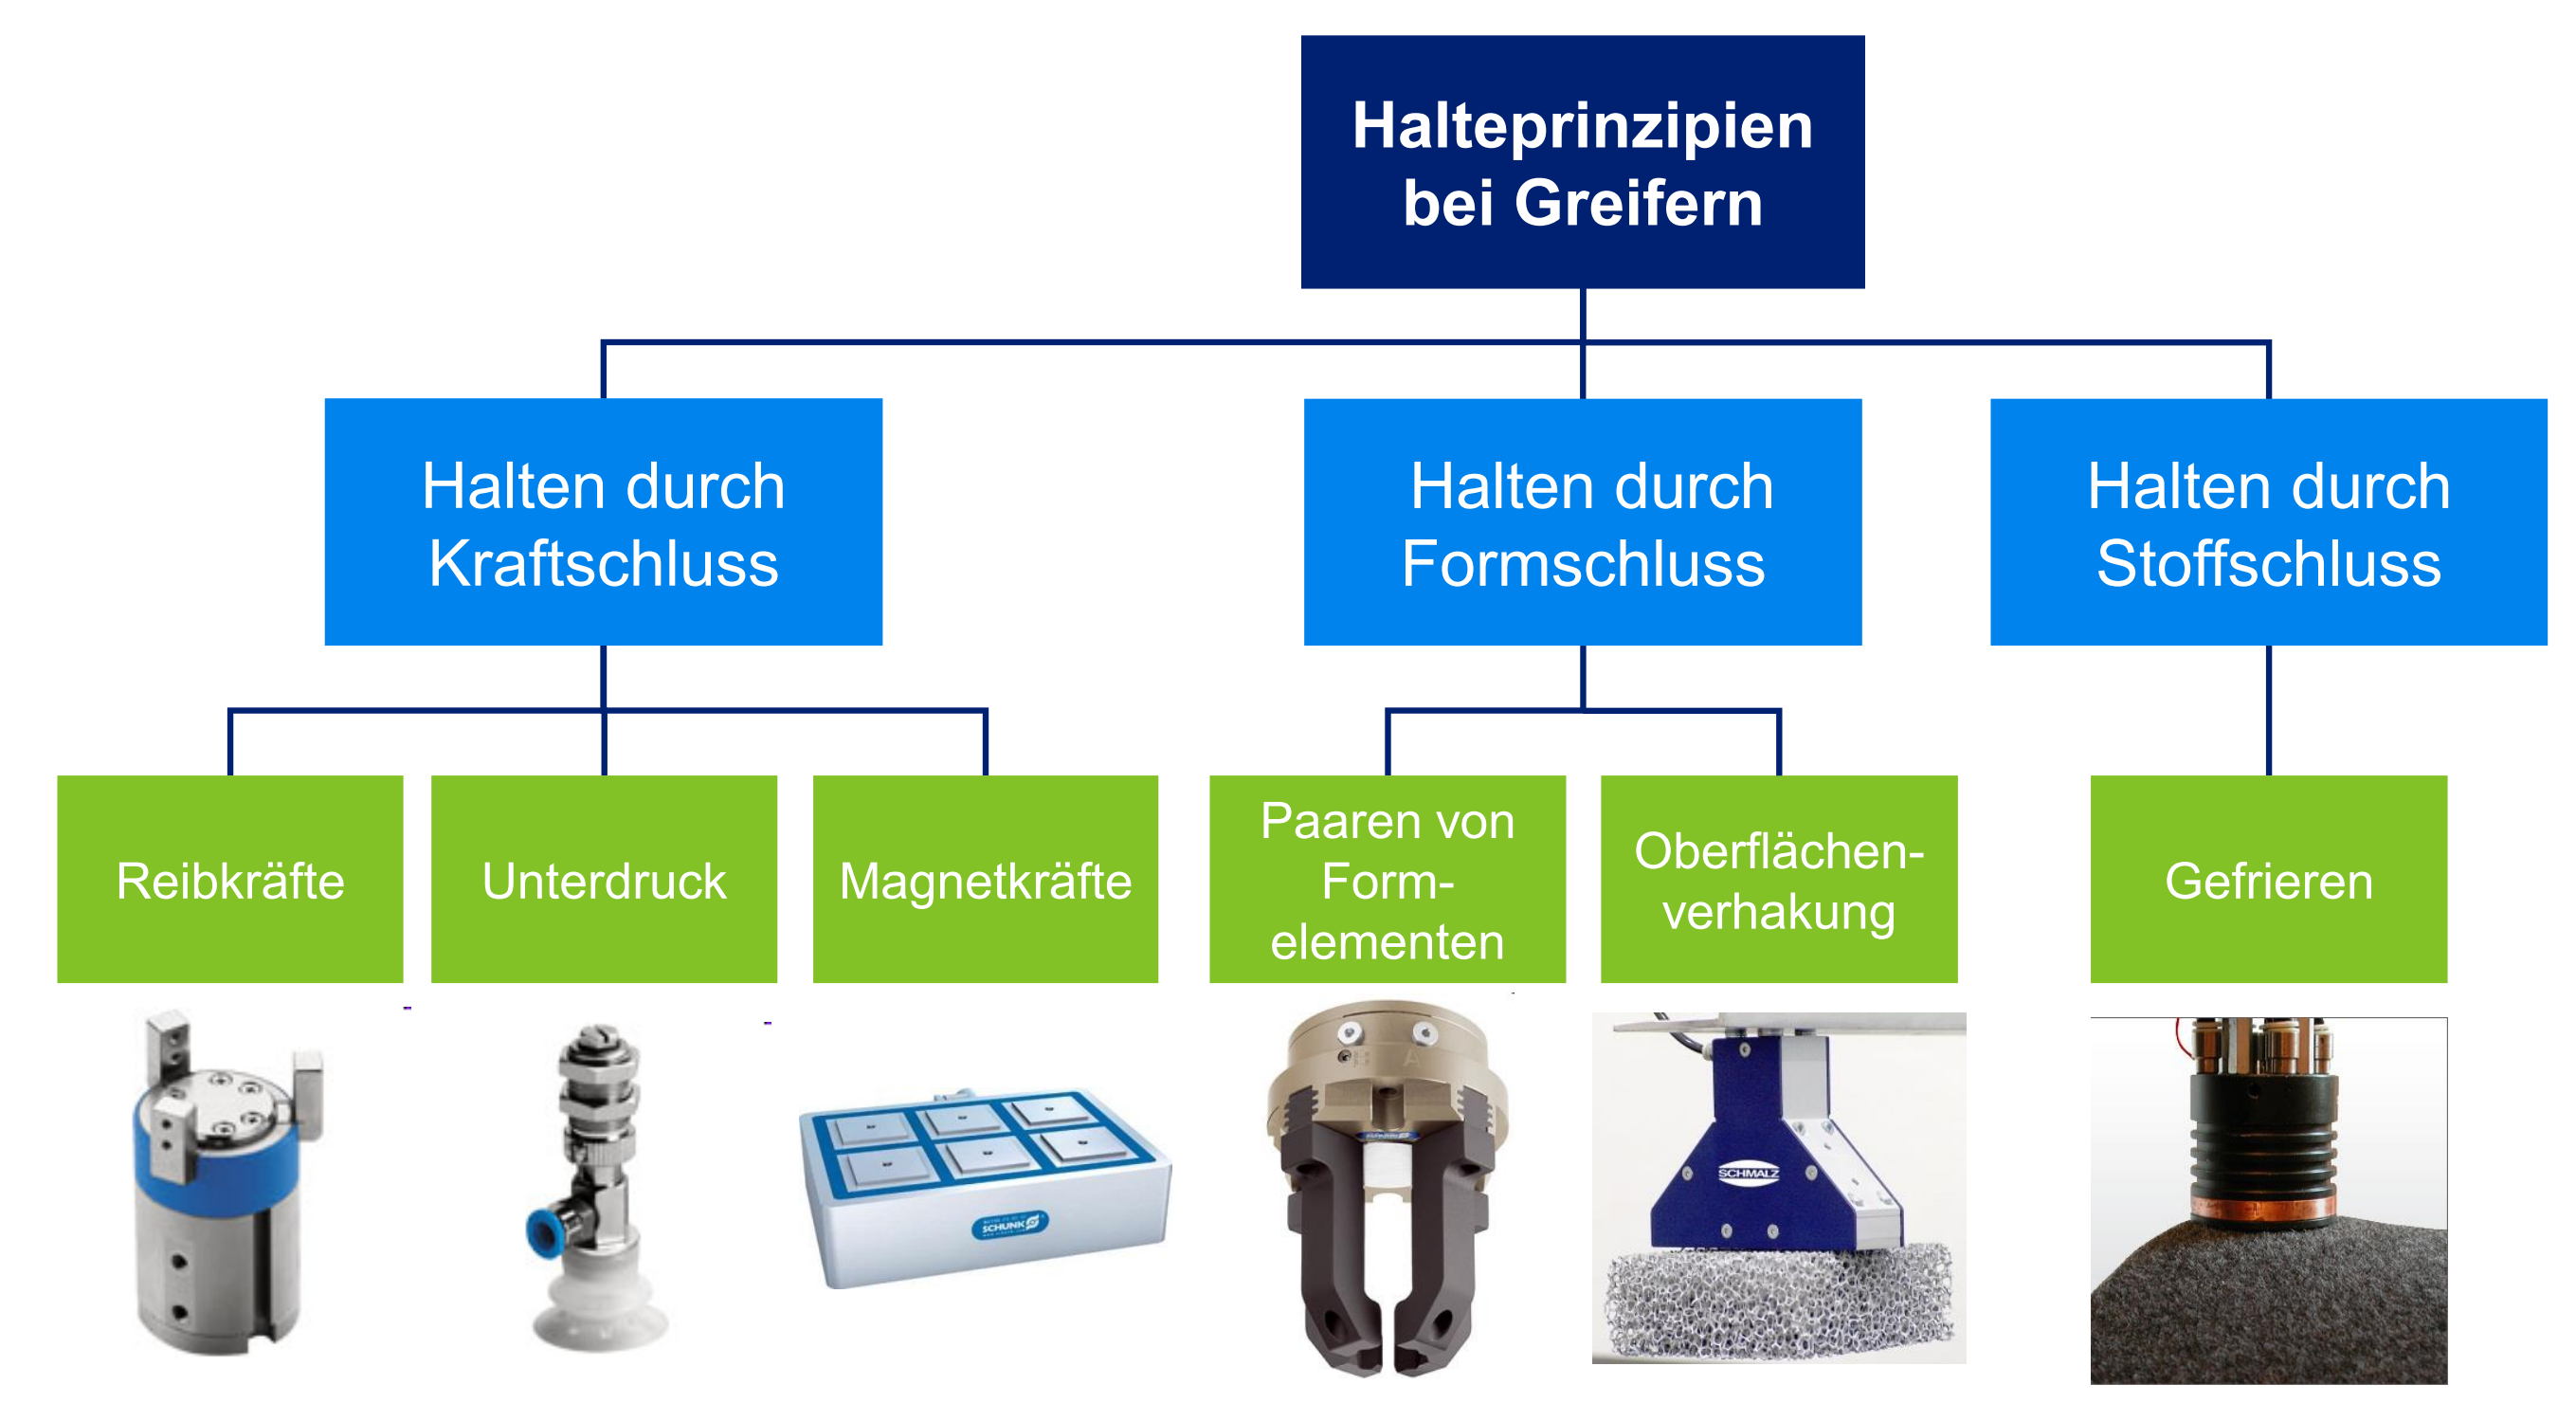
\includegraphics[width=0.8\textwidth]{halteprinzipien.png}
  \caption{三种夹爪形态的示例}
  \label{fig:halterprinzipien}
\end{figure}

光有夹爪还不够，实际生产中还需要以下这些装置来辅助完成任务：
\begin{itemize}
    \item 自动换爪系统：当机器人需要频繁切换不同的夹爪或工具时，可以在机器人手腕和工具之间加一块"适配板"，任务变了就自动换一套工具，不用人工去拧螺丝换夹爪。
    \item 碰撞保护装置：适配板之间靠气压支撑，正常工作时是刚性连接，一旦工具意外碰撞受到过载，气压结构会自动松开缓冲，避免损坏机器人或工件。
    \item 位置补偿装置：在装配这类需要高精度对准的工序中，补偿装置能允许末端执行器在小范围内自由浮动、自动纠正位置和角度偏差，同时又能防止绕装配轴转动跑偏，特别适合精密插装、螺丝拧入这类任务。
\end{itemize}

\paragraph{机器人周围的安全防护}

工厂里必须要有防护装置把人和机器人的工作区域隔开或及时停机。这些防护装置按方式可以分为两大类：
\begin{itemize}
    \item 隔离型防护：物理上把人挡在机器人工作区之外。比如围栏、安全门。
    \item 非隔离型防护：靠感知或操作方式来保证安全。比如安全垫（人一踩上去触发停机）、激光扫描仪（探测到人进入危险区并立即停机）、双手按钮开关（必须同时用两只手按下才能启动，防止手伸进危险区）。
\end{itemize}

\subsection{轨迹规划}

机器人要完成一个动作，在有了夹爪和骨架之后，还得进行\textbf{轨迹规划（Bahnplanung）}，它要做的就是从几何角度把一个运动任务描述清楚：路径约束、时间约束、机器人自身约束。

规划好的轨迹要变成机器人真正的运动，中间要经过几道工序，称为\textbf{面向指令段的轨迹控制（satzorientierten Bahnsteuerung）}。大致分四步：
\begin{enumerate}
    \item \textbf{为指令段做准备（Satzvorbereitung）}：把编程时的几何数据和运动学数据整理成数学函数
    \item \textbf{轨迹插补（Bahninterpolation）}：计算出轨迹上具体的点
    \item \textbf{坐标变换（Koordinatentransformation）}：把这些点从直角坐标系转换成机器人每个关节该转的角度值
    \item \textbf{位置控制（Lageregelung）}：把这些角度值作为目标值交给位置控制器去驱动电机实际执行。
\end{enumerate}

机器人的运动方式主要有三种。
\begin{itemize}
    \item \textbf{点位控制（PTP，Point to Point）}：只规定起点和终点，中间走的具体路径形状不确定，简单快速，常用于不要求路径形状的搬运任务。
    \item \textbf{多点控制（MP）}：通过预先采样、记录一系列密集的路径点来描述一条复杂曲线，常用示教/回放的方式编程。
    \item \textbf{连续轨迹控制（CP，Continuous Path）}：整条路径的位置和姿态在全程都被精确规定，常见的插补方式有直线、圆弧、样条曲线，其中直线轨迹最常用，比如装配这类需要精确路径的场合。这些插补方式如图 \ref{fig:interpolation} 所示。
\end{itemize}

\begin{figure}[htbp]
  \centering
  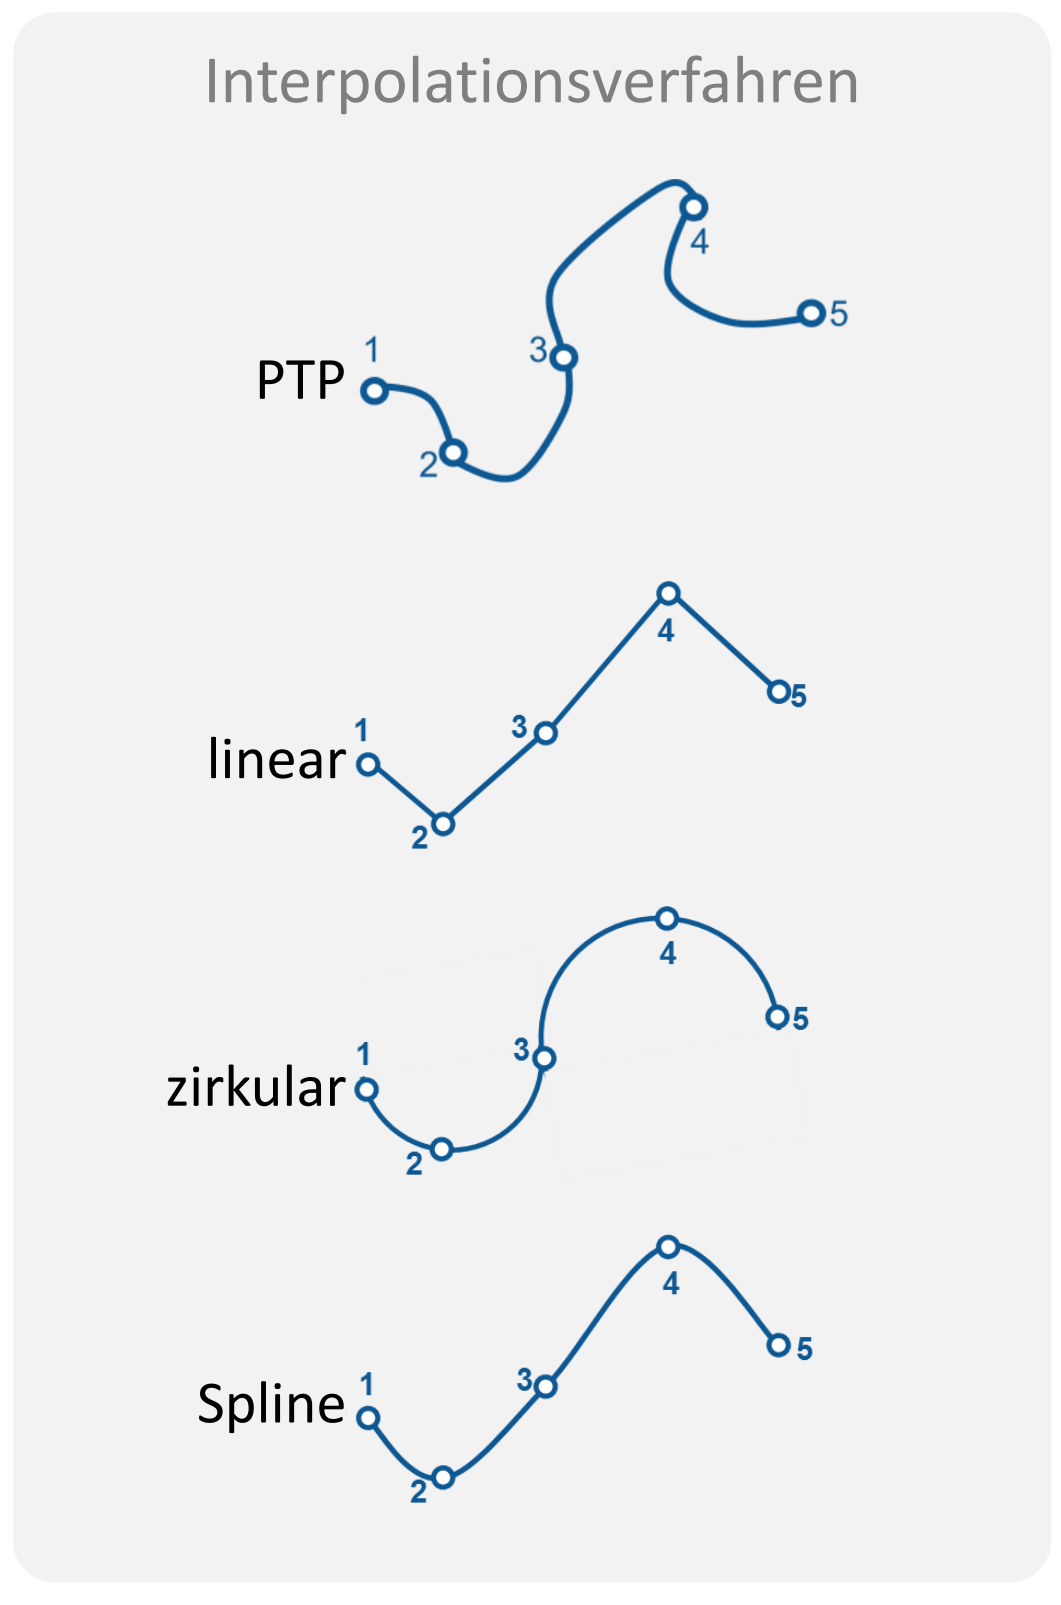
\includegraphics[width=0.35\textwidth]{interpolation.png}
  \caption{三种夹爪形态的示例}
  \label{fig:interpolation}
\end{figure}


\subsection{编程方法}

\subsubsection{在线编程}

在线编程的特点是直接在真实机器人上进行示教，主要有两种做法。
\begin{itemize}
    \item 示教编程（Teach-In）：如图 \ref{fig:teachin} 所示，操作人员用一个操作手柄，把机器人依次移动到任务需要的几个关键位置，每到一个位置就把该点的坐标连同相关参数（比如用哪种插补方式、走多快）一起存下来；正式运行程序时，机器人就按顺序依次开到这些存好的点，并套用当时记录的参数。
    \item 引导编程（Playback）：如图 \ref{fig:playback} 所示，不是一个点一个点地示教，而是直接拉着机器人的手走完整个动作，比如靠装在末端执行器上的力矩传感器感知人手的推力，或者靠一个运动学替代模型来跟随人的动作，机器人会把整个连续的运动过程记录下来，之后原样重放。
\end{itemize}
这两种方式的共同优点是直观、不需要专业编程知识，缺点是要占用真实机器人的时间，示教期间机器人没法干别的活。

\begin{figure}[htbp]
    \centering
    \begin{subfigure}[b]{0.46\textwidth}
        \centering
        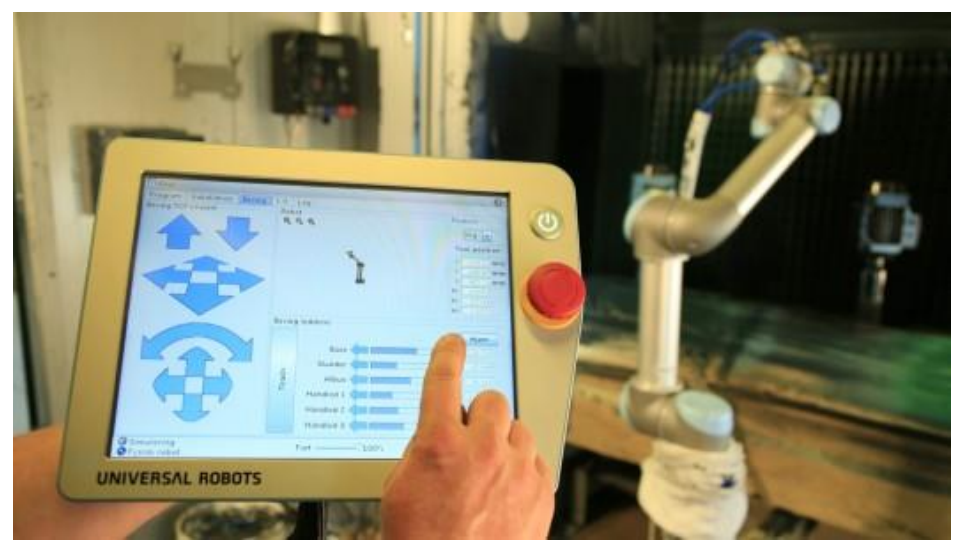
\includegraphics[width=\textwidth]{teachin.png}
        \caption{示教编程 Teach-in}
        \label{fig:teachin}
    \end{subfigure}
    \hfill
    \begin{subfigure}[b]{0.49\textwidth}
        \centering
        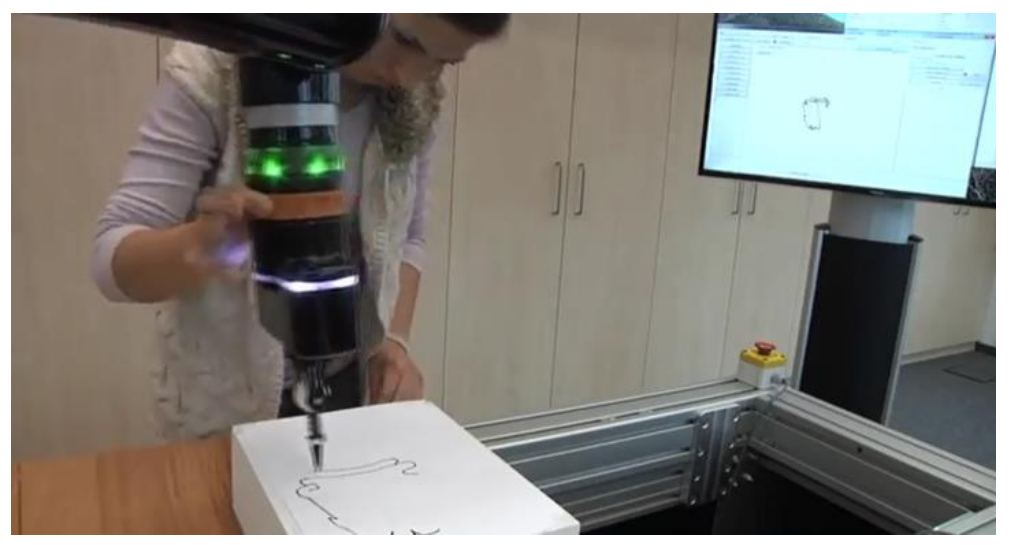
\includegraphics[width=\textwidth]{playback.png}
        \caption{引导编程 Playback}
        \label{fig:playback}
    \end{subfigure}
    \caption{在线编程方法}
    \label{fig:onlineprogramming}
\end{figure}

\subsubsection{离线编程}

离线编程不需要占用产线上的真实机器人，如图 \ref{fig:offlineprogramming} 所示。

\begin{figure}[htbp]
  \centering
  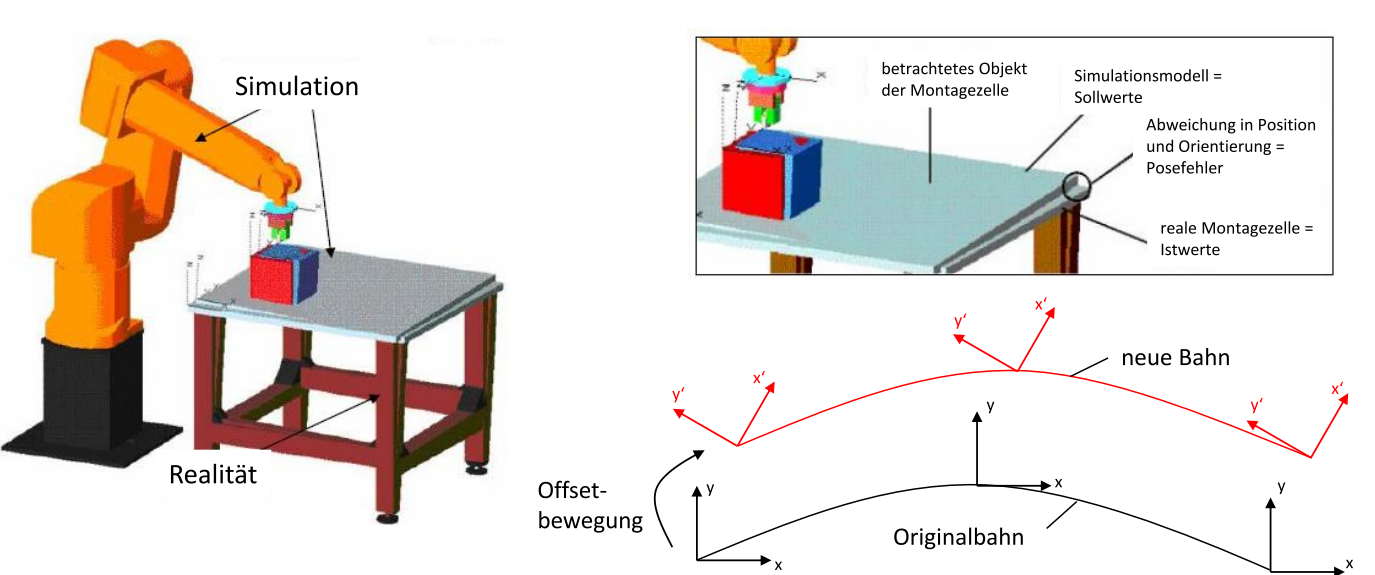
\includegraphics[width=0.8\textwidth]{offlineprogramming.png}
  \caption{离线编程案例}
  \label{fig:offlineprogramming}
\end{figure}

离线编程也是有两种做法：
\begin{itemize}
    \item 文本编程：直接用文字代码写程序，因为只需要一个编辑器，投入成本很低；不过问题在于几乎每个机器人厂商都有自己的一套编程语言，彼此互不兼容。
    \item 基于仿真的编程：先在电脑里把整个加工单元（工作台、零件、机器人等）建模出来，规划好机器人大致怎么运作，再通过设置一系列途经姿态（Via-Pose）来编写机器人的运动路径。
\end{itemize}

仿真模型里规划的路径搬到真实产线上执行时，因为设备安装误差、零件实际位置和仿真设想的不完全一致等原因，机器人实际走的位置和姿态往往会和理论值有偏差（姿态误差）。为了解决这个问题，通常先在仿真环境里把整套系统规划出来，然后把真实设备搭建起来，接着对真实产线进行实测标定，最后根据标定结果反过来修正仿真模型，或者给机器人的原始轨迹加一个偏移量，让仿真规划出来的路径在真实世界里也能精确复现。


\subsubsection{混合编程}

在线和离线各有短板，混合编程就是把两者结合起来，先用示教在真实机器人上快速确定出几个关键位置，锚定住任务的大致框架，然后再用离线的方式去补充和精细化：一种做法是用示教编程定好关键点后，再用文本代码把中间的逻辑、参数补全；另一种做法是用示教编程定好关键点后，再放到仿真环境里做进一步的路径优化和碰撞检查。这样既保留了示教所见即所得、贴近真实情况的优点，又能用离线手段做更精细的编辑和验证，减少了纯离线编程常见的仿真与现实偏差问题。


\subsection{智能化融入}
\label{subsec:intelligent}

前面几节讲的都是机器人本身，它长什么样、怎么动、怎么编程。这一节换了个角度，讲的是怎么把机器人聪明地安排进一条有人参与的生产线，让人和机器人各自发挥所长、协同完成任务。

\paragraph{示例：飞机隔框铆接}

如图 \ref{fig:nietprozess} 所示，原来的做法是两名工人手持铆枪和顶把，把大量铆钉一颗颗打进隔框，把它和机身段连接起来。这个工作又累又不符合人体工学，因为它经常需要将手臂举过头顶作业，铆钉数量又多，是个很适合重新设计、引入自动化辅助的场景。

\begin{figure}[htbp]
  \centering
  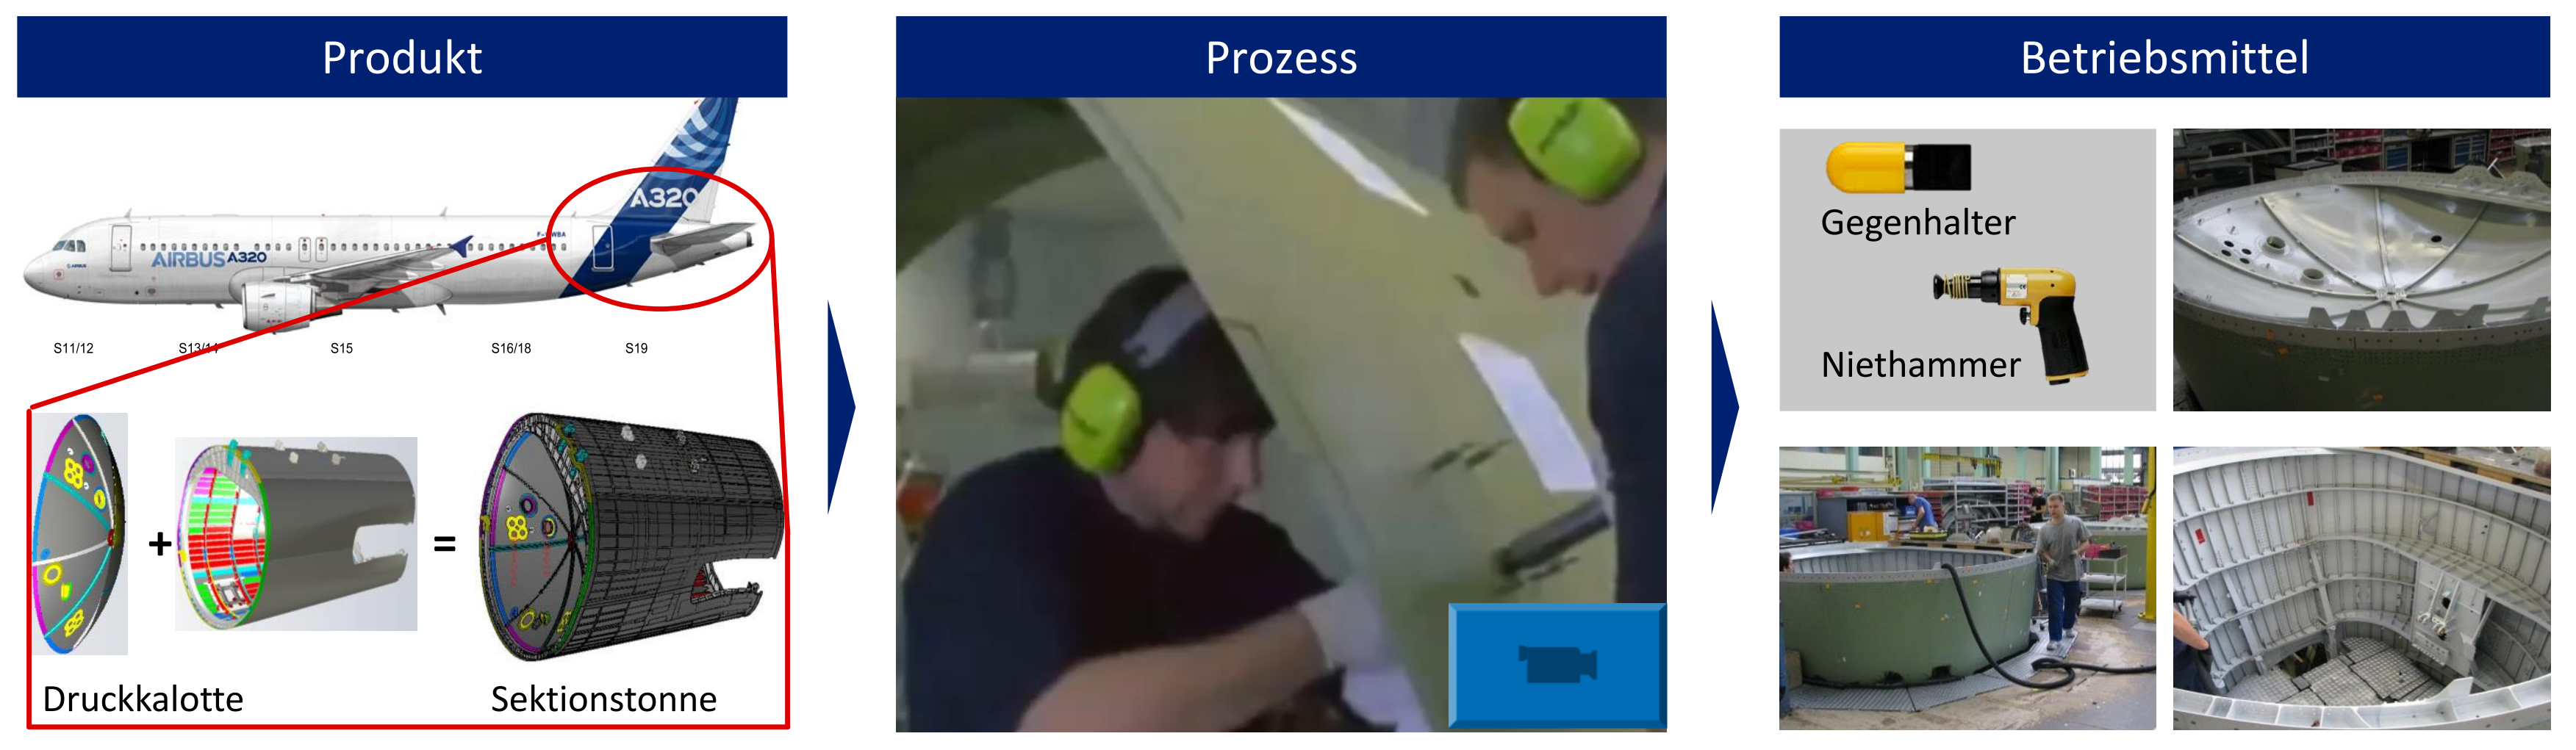
\includegraphics[width=1\textwidth]{nietprozess.png}
  \caption{飞机隔框铆接的原始方法}
  \label{fig:nietprozess}
\end{figure}

要把人和机器人智能地组合到一条产线里，大致分六步：
\begin{enumerate}
    \item 流程规划与方案设计，明确任务该分给人还是机器人
    \item 建一个虚拟模型，把产品、工艺、设备信息都参数化地描述出来
    \item 做产线配置，把规划好的方案在现实中搭建起来并标定
    \item 设计，让工人能方便地了解和调整系统
    \item 实际操作运行
    \item 工艺执行
\end{enumerate}
这六步环环相扣，前一步的结果是后一步的输入。接下来将详细解释每一个步骤是如何实现的。

\paragraph{第一步：流程规划与方案设计}

方案设计的核心是能力匹配（Mapping）：先梳理出这项任务实际需要哪些能力，再对比人和机器人各自能提供哪些能力，把两者匹配起来，形成几种备选方案。总体来看，人的优势在于灵活，短板是对工艺的把控不够精确、容易受人体工学限制。机器人恰好相反：能严格按照设定路径精确移动、可靠地重复执行单调任务、结果一致性好；短板是产品设计必须迁就自动化要求，也不像人一样灵活应变。

放到铆接案例里，工人负责铆接任务里需要灵活操作、经验判断的部分，机器人则负责单调但需要稳定输出力的部分。所以外面的人操作铆枪，里面的机器人稳稳地顶住，两者配合完成铆接。

\paragraph{第二步：虚拟模型}

有了分工方案后，就可以搭建一个虚拟模型，参数化地记录。这是为了能提前在电脑里对方案做分析、验证和优化，减少后续返工的风险。

\paragraph{第三步：产线配置}

把实际需要的设备搭建到位，再通过测量确定它们真实的位置和朝向，这称之为\textbf{标定}，然后把这些实测数据反馈回虚拟模型里，让虚拟模型和现实情况对齐。机器人的实际控制就可以基于这个校准过的虚拟模型来进行。

标定本身还可以分三个层级，如图 \ref{fig:konfiguration} 所示：
\begin{figure}[htbp]
  \centering
  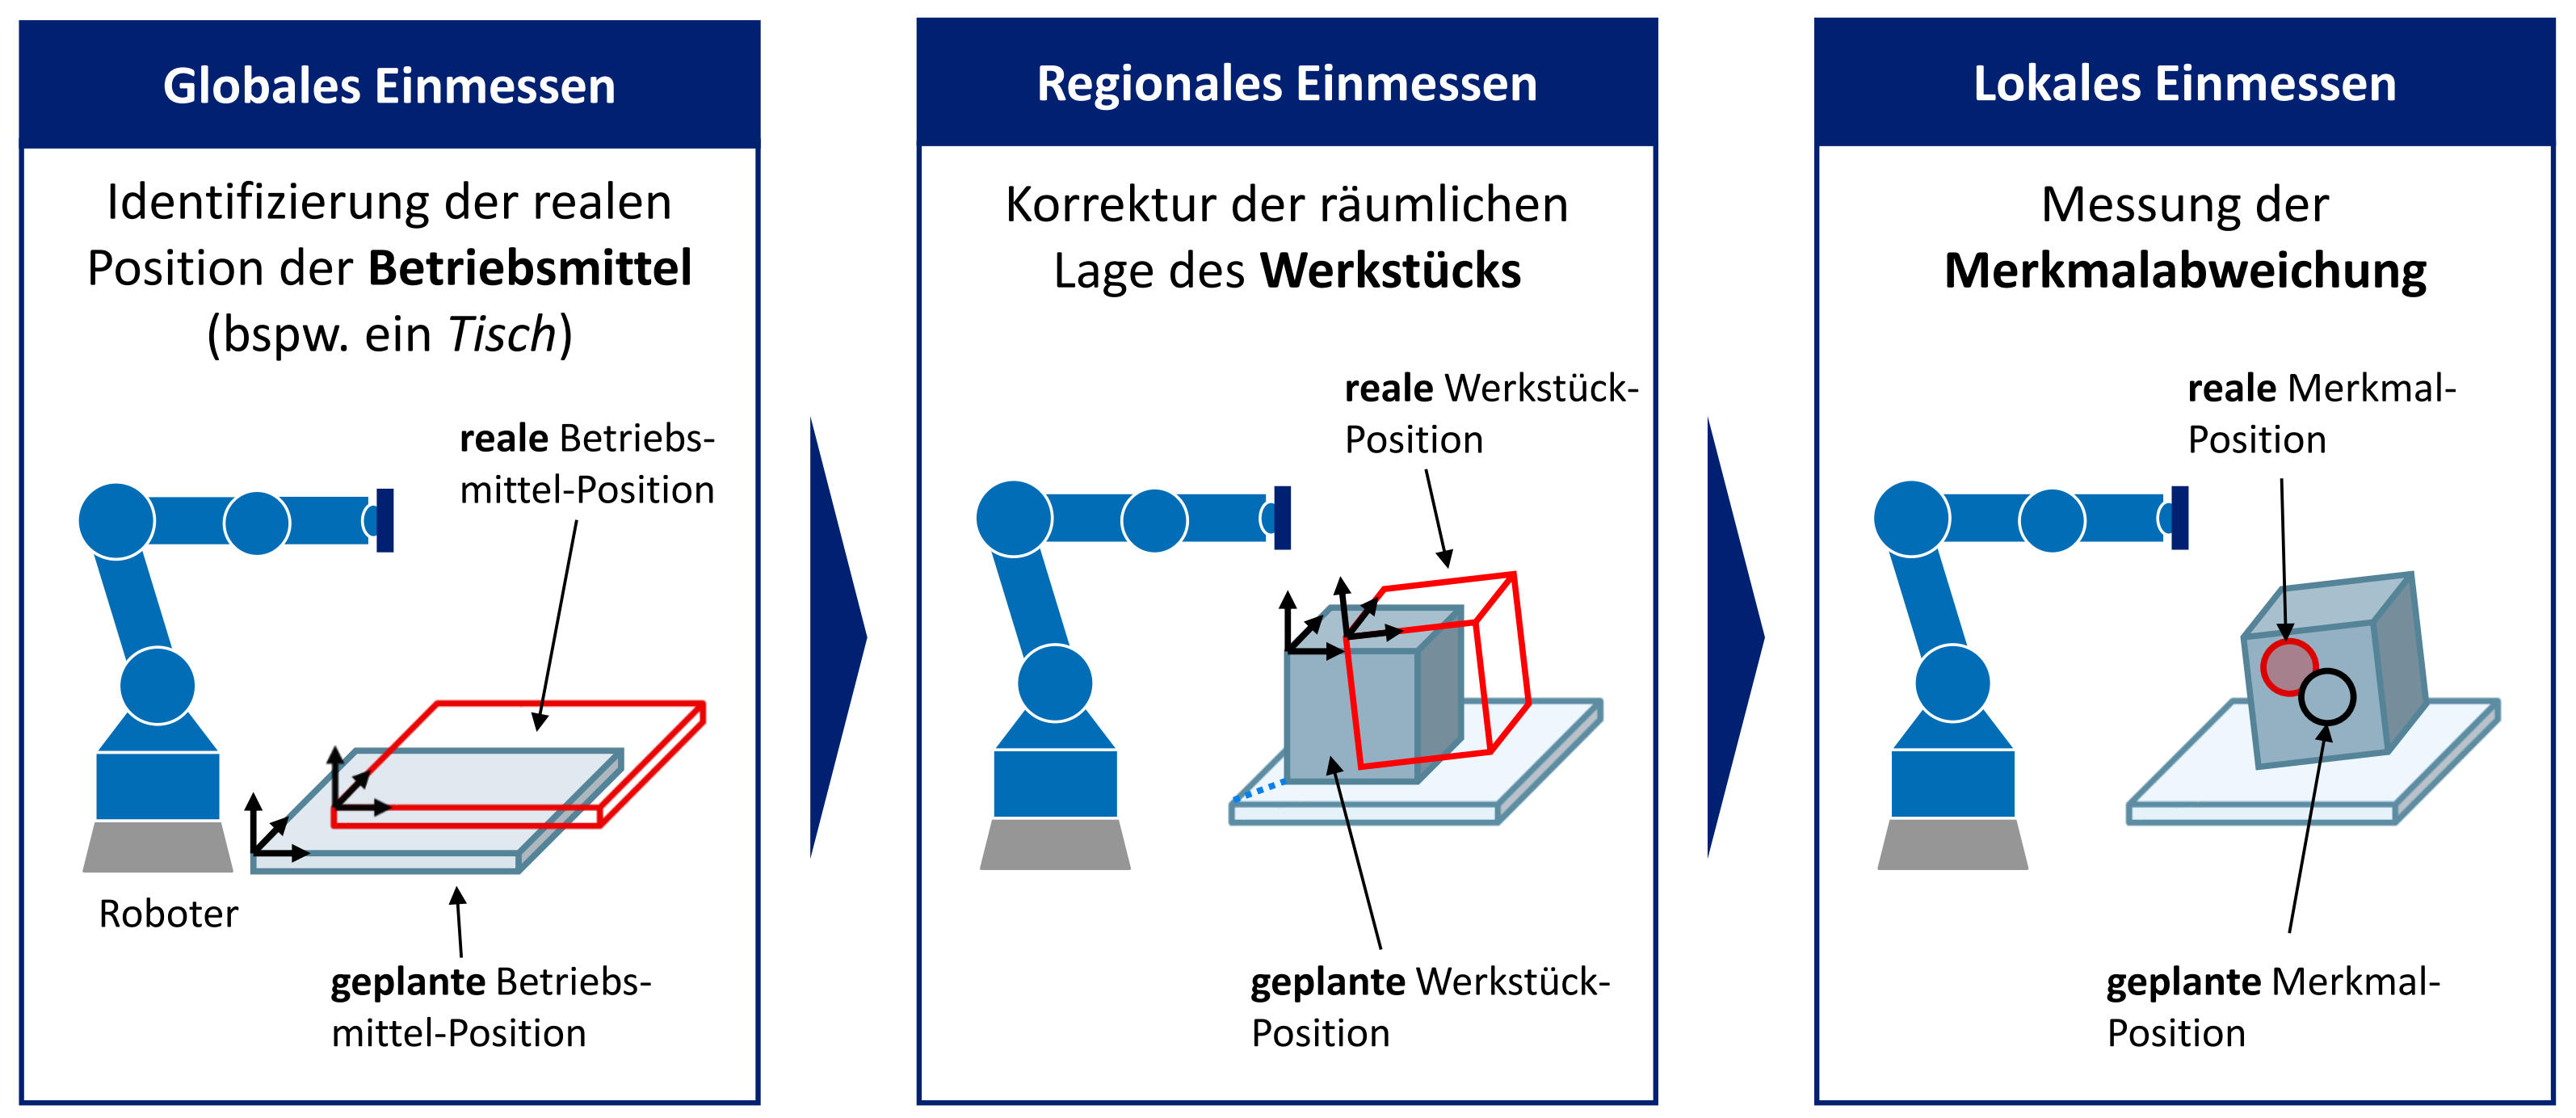
\includegraphics[width=0.8\textwidth]{konfiguration.png}
  \caption{标定的三个层级}
  \label{fig:konfiguration}
\end{figure}
\begin{itemize}
    \item \textbf{全局标定（Globales Einmessen）}：确定大件设备（比如工作台）在空间中的整体位置；
    \item \textbf{区域标定（Regionales Einmessen）}：修正某个工件本身摆放位置的偏差；
    \item \textbf{局部标定（Lokales Einmessen）}：进一步测量工件上具体特征点（比如某个铆钉孔）的精确偏差。
\end{itemize}
层级越细，精度要求也越高。案例中就用到了区域标定：用线激光三角测量传感器识别隔框上的铆钉孔图案，据此计算出一个局部坐标系，用来修正真实工件和CAD模型之间的偏差，进而推算出其余铆钉孔的准确位置，供机器人后续铆接使用。

\paragraph{第四步：人机交互界面}

产线上的工人往往不懂机器人编程，但生产中经常需要根据新的产品变型或流程优化去调整机器人程序。解决办法是给工人提供直观的操作界面和仿真环境，让他们不需要专业编程知识也能修改任务，调整结果还会实时反馈给工人确认。

\paragraph{第五步和第六步：实际操作运行工艺执行}

系统运行起来后，工人应当能在生产过程中随时进行简单的干预，比如用语音喊启动/停止来控制流程推进到下一步，不需要复杂培训就能上手，也让工人对整个流程更有掌控感、更容易接受这套人机协作方式。
% !TeX root = main.tex
\section{工业机器人II}

\subsection{人机协作}

\ref{subsec:intelligent} 小节中，我们通过飞机铆接案例提到，工业机器人和人各有各的长处和短板。传统自动化生产线的做法是把人和机器人彻底隔开。工业4.0描述的人机协作则完全不同，它让人和机器人共用同一个工作空间协同作业，这就要求系统必须能可靠地识别和追踪人的位置，对整个工作空间进行实时监控，一旦有风险就能及时反应。这种方式能支持更灵活的生产流程，不用像传统产线那样改流程就要改设备。

人和机器人在同一空间里干活，紧密程度可以从完全分离到完全合体分成五个等级，如图 \ref{fig:zusammenarbeitsgrade} 所示。

\begin{figure}[htbp]
  \centering
  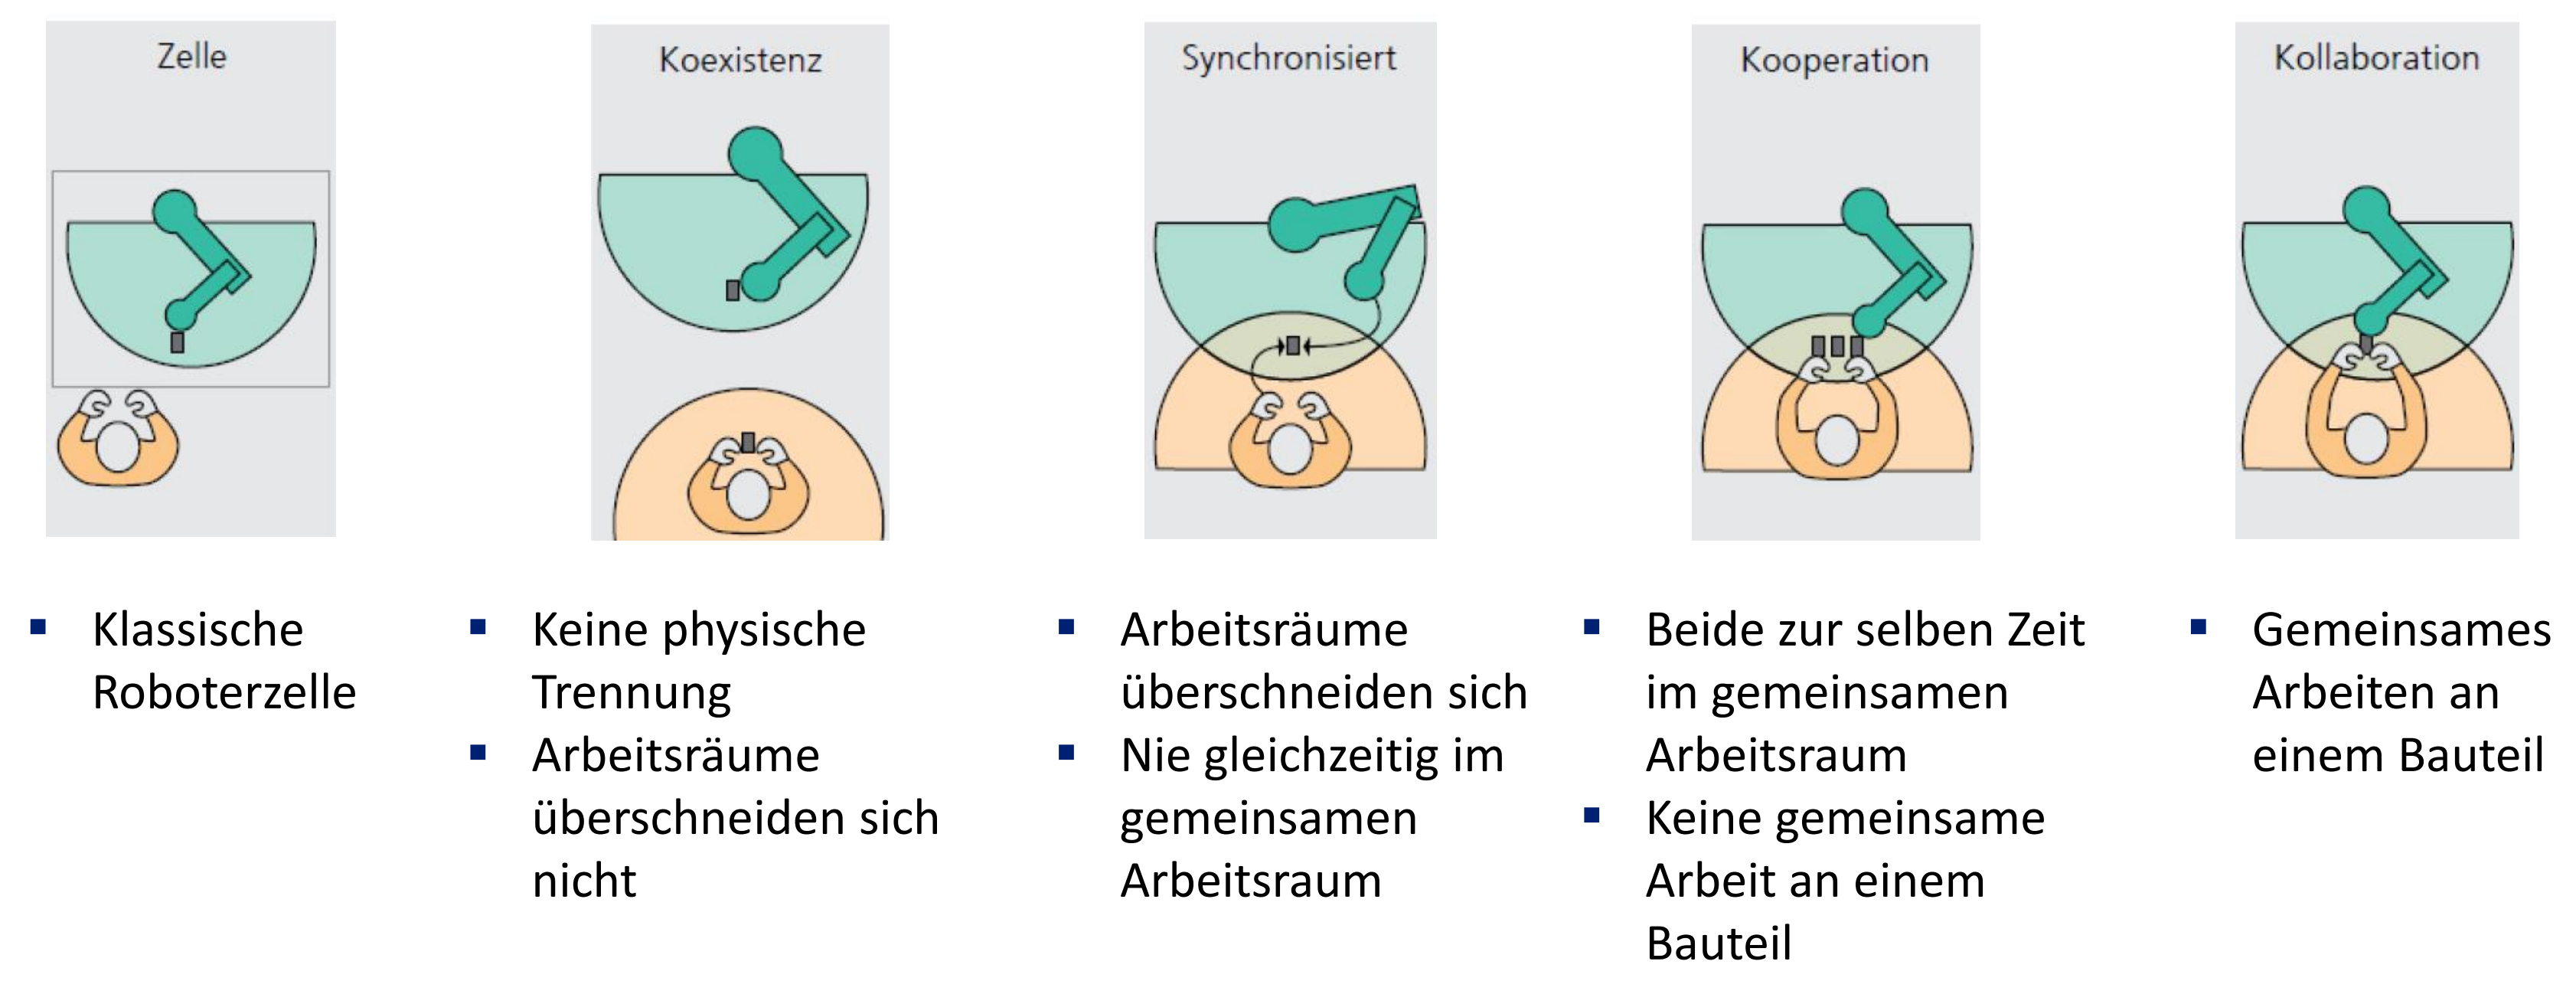
\includegraphics[width=1\textwidth]{zusammenarbeitsgrade.png}
  \caption{人机协作的五个等级}
  \label{fig:zusammenarbeitsgrade}
\end{figure}

\begin{enumerate}
    \item \textbf{单元（Zelle）}：机器人被围栏围住，和人的工作区完全分离。
    \item \textbf{共存（Koexistenz）}：人和机器人之间没有围栏，但各自的工作范围依然不重叠。
    \item \textbf{同步（Synchronisiert）}：两者的工作范围开始出现重叠，但系统会保证他们不会同时出现在这个重叠区域里。
    \item \textbf{合作（Kooperation）}：人和机器人可以同时出现在共同的工作空间里，但不会共同操作同一个工件。
    \item \textbf{协作（Kollaboration）}：人和机器人共同对同一个工件进行操作。
\end{enumerate}

要实现比较高等级的人机协作，最大的挑战是系统要能把传感、感知和反应整合到一起，实时应对生产过程中各种不确定的变化。要做到这一点需要执行机构、传感器和智能软件三者高度配合协调，还需要引入性能足够强的传感器以及配套的数据处理算法，才能让机器人看得懂周围发生了什么、反应得过来。


\subsection{安全规范与概念}

既然人和机器人要共用一个空间，就必须保证人的安全。分成本质安全设计，从机械结构本身入手，比如让机器人边缘更圆滑、材质更软；另一条是功能安全，靠传感器、控制器这些主动防护功能来实时监测和响应危险。

机械安全标准分三个层级，像金字塔一样，如图 \ref{fig:sicherheitsnormen} 所示。
\begin{itemize}
    \item A类标准讲的是最基础的安全设计原则；
    \item B类标准是某一类通用安全技术要求；
    \item C类标准针对具体某一类机械给出非常具体的安全要求
\end{itemize}
层级越往上越具体、越贴近实际应用。

\begin{figure}[htbp]
  \centering
  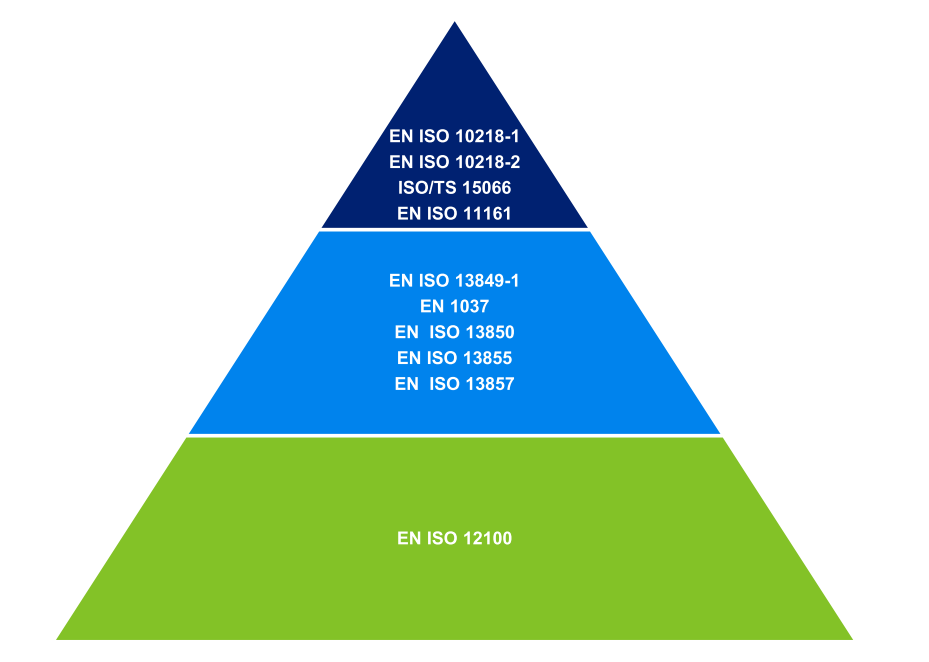
\includegraphics[width=0.5\textwidth]{sicherheitsnormen.png}
  \caption{专门为人机协作设计的机器人产品}
  \label{fig:sicherheitsnormen}
\end{figure}

\paragraph{DIN EN ISO 10218：机器人的基本安全标准}

这份标准分两部分。第一部分针对机器人本体，规定了工业机器人和机器人系统特有的危险源，以及对机器人本身（作为系统的一个组成部分）的安全要求。第二部分针对机器人系统与集成，规定了机器人被集成到产线或工作单元时会带来的额外风险，以及在集成安装过程中如何保证安全。

\paragraph{ISO/TS 15066：专门为人机协作补充的规范}

ISO/TS 15066是2016年发布的技术规范，专门针对协作机器人系统的设计。它一方面讲怎么设计协作应用、怎么做危险识别和风险分析，另一方面给出了协作应用需要满足的具体要求，包括安全功能设计、协作工位怎么布置、协作机器人怎么使用和运行。

ISO/TS 15066规定了四种能保证人机安全共处的方法，实际应用中常常组合使用。

方法一是\textbf{安全定向停止（Sicherheitsgerichteter Halt）}：人进入协作空间前，机器人必须先进入安全停止状态。本质上人只能在机器人完全静止时才能靠近它，所以不可能发生碰撞。

方法二是\textbf{手动引导（Handführung）}：同样要求人进入协作空间前机器人先停止，然后激活手动引导模式，这时机器人只能被人用安全的、大幅降低的速度手动操纵。也就是说人始终只能接触静止或被自己缓慢操控的机器人。

方法三是\textbf{速度和间距监控（Geschwindigkeits- \& Abstandsregulierung）}：这是唯一允许机器人和人同时在协作空间内运动的方式。系统会实时监测人和机器人之间的距离，机器人的速度会随着这个距离动态调整。离得越近走得越慢，距离足够小就会停下。这里安全距离的计算遵循（EN ISO 13855）：
\begin{equation}
    S = (K × T) + C
\end{equation}

其中 $S$ 是最小安全距离（mm），$K$ 是人接近的速度参数（mm/s），$T$ 是整个系统的反应加制动时间（s），$C$ 是额外的侵入余量（mm）。这个公式假设机器人是静止的、只有人在移动。

TS 15066在此基础上给出了更精细的动态计算公式，把机器人自身的运动也考虑了进去：
\begin{equation}
    s_p(t₀) = s_h + s_r + s_s + c + z_d + z_r
\end{equation}

其中 \(s_h\) 是人的位移量（mm）、\(s_r\) 是机器人的位移量（mm）、\(s_s\) 是机器人的制动距离（mm）、c 是侵入余量（mm）、\(z_d\) 和 \(z_r\) 分别是人和机器人位置的测量不确定度（mm）。相比前一个公式，这个版本同时考虑了人和机器人双方都在运动、以及定位误差带来的不确定性，算出来的安全距离更贴近人机协作的真实场景。

方法四是\textbf{功率和力限制（Kraft- \& Leistungsreduzierung）}：这是唯一允许人和机器人发生物理接触的方式，靠的是机器人本身在结构设计上就足够温和，再叠加安全功能来降低风险。
\section{人机交互}

\subsection{互动与沟通}
\label{subsec:kommunikation}

互动与沟通这两个词经常混用，但严格来说不完全一样。

\emph{沟通（Kommunikation）} 指的是信息的传递或交换，可以是一个动作加一个反应，也可能只是单向的信息发出。而且沟通不一定是故意的，很多时候我们是无意识地在传递信息（比如你皱了下眉头，别人就接收到了）。

\emph{互动（Interaktion）}强调的是人与人之间的相互作用。互动一定是双向的：你做了动作，对方也做出反应，这一来一回构成了互动。

两者有很大的重叠，但互动更强调"来回"，沟通更强调"信息本身"。

\paragraph{Watzlawick 的五条沟通公理}

这是沟通学里最著名的理论之一，由心理学家 Paul Watzlawick 提出。
\begin{enumerate}
    \item 人不可能不沟通，哪怕你一言不发，你的沉默、表情、姿态本身也在传递信息。
    \item 每条信息都有两层含义：一是"内容层面"（你说的事实是什么），二是"关系层面"（你和听者之间是什么关系，语气亲密还是疏远）。
    \item 人类沟通同时用两种语言：一种是数字化的，逻辑清晰、有语法规则（比如说出来的话本身）；另一种是模拟化的，靠语气、表情、肢体动作传达关系层面的含义。
    \item 沟通是循环的因果关系——你说的话是对方反应的原因，对方的反应又成了你下一句话的原因，很难说谁是"起点"。
    \item 沟通要么是对称的，要么是互补的。对称是双方地位平等（比如朋友间的争论），互补是双方地位不对等（比如老师和学生）。
\end{enumerate}

\paragraph{Schulz von Thun 的沟通四层模型}

德国心理学家 Schulz von Thun 提出：你说的每一句话，其实同时包含四层信息：
\begin{enumerate}
    \item 事实信息：你客观陈述的内容是什么
    \item 自我表露：这句话无意中透露了你自己的什么状态或想法
    \item 关系暗示：这句话透露出你怎么看待对方、你们是什么关系
    \item 诉求：你说这句话，其实是想让对方做点什么
\end{enumerate}
经典例子是副驾驶对司机说前面是绿灯。表面上只是在陈述一个事实，但背后可能同时是我有点着急（自我表露）、我觉得你反应有点慢（关系暗示，可能让人不爽）、你可以走了（诉求）。同一句话，说话人的意图和听话人的理解经常对不上，这就是很多沟通误会的根源。

\paragraph{Jones \& Gerard 的四种社会互动模式}

这个理论描述了两个人互动时，各自到底在"跟随"什么：
\begin{enumerate}
    \item 完全互动：双方的目标和行为高度一致，配合得很好。
    \item 非对称互动：一方完全按自己的节奏来，不太理会对方。
    \item 伪互动：表面在互动，实际上双方都只顾着实现自己的目标，没有真正配合。
    \item 反应式互动：只是被动地对对方的刺激做出反应，没有自己的主动计划。
\end{enumerate}

这一节看似在讲人与人之间的沟通理论,但其实是为后面几节做铺垫。接下来会讲人和机器之间怎么互动，机器要模拟或应对人类沟通里的这些层次和模式，才能设计出好用的人机交互系统。理解人与人之间沟通的复杂性，是理解人机交互设计难点的第一步。

\subsection{人与机器的沟通}
\label{subsec:contactmanmachine}

沟通要发生，需要两个基本前提：
\begin{itemize}
    \item 共同的符号库（gemeinsamer Zeichenvorrat）：双方得用同一套语言或符号系统,不然收到信号也看不懂。比如只听得懂一种语言的人，收到用另一种语言的信息，是完全无法理解的。
    \item 通道和兼容的收发器官：得有一条信息能传过去的路径，双方的发送和接收设备也得匹配。
\end{itemize}
信号（Signal） 是信息的载体，可以是一个或多个符号，它的作用是在接收方那里触发某种反应。但同一个信号，不同接收者的反应可能完全不同，这取决于对方的知识、经验、教养、文化背景。人、动物、机器面对同一个信号，做出的反应逻辑也各不相同：人可能是本能反应，也可能是后天学来的行为模式和约定俗成的规则；机器则是靠预先设定的定义和规则来"反应"。

\paragraph{Shannon \& Weaver 的发送者-接收者模型}

这是信息论里最经典的模型之一,把一次沟通拆成几个环节：

信息源 → 发送者（编码） → 信号 → 传输通道 → 接收者（解码） → 目标

发送者把要传达的信息编码成信号，信号通过通信信道传输（传输过程通常会受到干扰），接收者把收到的信号解码还原成信息。

\emph{干扰（Störungen） 的来源}：
\begin{itemize}
    \item 信道里的信号叠加（噪声）
    \item 解码过程中的错误
    \item 双方符号库不完全兼容
\end{itemize}

\vspace{2em}

沿用 Shannon \& Weaver 的框架，\emph{沟通可以从三个层面来分析}，每个层面回答一个不同的问题：
\begin{itemize}
    \item \emph{技术层面（technical）}：符号有没有被正确传输？关注编码、解码和物理层面的信号传递本身。比如一个信号灯，是把电流转换成光信号、光波传播出去、再被视网膜转换成神经信号的过程。
    \item \emph{语义层面（semantic）}：传输的符号有没有精确传达出想表达的含义？关注符号的形式含义和内容组合。比如信号灯的颜色约定：红色=故障（加工中断）、黄色=警告（料仓存料少）、绿色=机器运行、蓝色=机器停止。
    \item \emph{效果层面（effectiveness）}：收到的信息有没有有效地引导出预期的行为？关注信息实际产生的效果。同样是信号灯，黄灯让员工去补料（有效），但如果员工看到红灯却在到处找故障原因而找不到（无效），说明信息虽然传到了，却没达成预期效果。
\end{itemize}
这三层递进的关系很重要：技术上传对了，不代表语义上双方理解一致；语义上理解一致，也不代表最终真的引导出了想要的行为。

沟通有三种主要形式：
\begin{itemize}
    \item 语言沟通（Verbale Kommunikation）：说出来的话、字母、数字、词语、句子和句法结构，主要负责传递事实信息，也带有一定的权重和强调。
    \item 副语言沟通（Paralinguistische Kommunikation）：不是“说了什么”，而是“怎么说”：语调、语速、停顿、笑声、叹气，这些提供了如何解读信息的线索。
    \item 非语言沟通（Nonverbale Kommunikation）：身体的动作和反应，包括触觉、身体距离、姿态、眼神接触、表情手势、着装风格等，主要用来表达情绪。
\end{itemize}
非语言沟通的难点在于它常常含糊不清、依赖上下文：同样是一声大喊，在庆典活动上是欢呼，在紧急情况下却是求救。脱离了场景，机器很难准确判断该如何理解。

工程标准上，沟通模型同样可以用 \ref{subsec:industrialcommunication} 小节中提到的 OSI 七层参考模型来表示。其中1、2层偏重传输本身，3层往上更偏向应用相关。在实际通信中，A站和B站之间的每一层都通过约定好的协议互相对应通信。发送方从第7层往下逐层封装，经过物理层传输后，接收方再从第1层往上逐层解封装还原。每一层之间都有明确定义的接口，各层之间互不干扰，这样才能让不同厂商、不同系统的设备也能互相听懂对方。

\subsection{技术可能性与限制}
\label{subsec:restriktoren}

前两节讲了沟通的理论模型。这一节我们落到实处：人有哪些发送器和接收器、机器有哪些对应的技术手段、这些渠道各自会遇到什么干扰，以及人和机器该如何互相迁就对方来实现有效沟通。

人的感官既是接收器，也是发送器。人身上天生自带一整套传感器（Sensorik）和执行器（Aktorik）：感知方面有视觉、听觉、嗅觉、味觉、平衡觉，以及触觉。表达方面，不同的感知渠道对应不同的表达方式：视觉对应表情和手势,听觉对应发声,触觉对应触摸、动作和身体姿态。人本身就是一套多模态的收发系统，这也是后面讨论机器如何与人沟通的基础——机器要跟人沟通，得对上人的这些感知渠道。

三种主要的传输方式：
\begin{itemize}
    \item 光学传输：机器靠指示灯、数码管显示、显示器发送，人靠眼睛接收。人靠表情、手势发送；机器靠摄像头接收。
    \item 声学传输：机器靠运行噪音、语音播放、蜂鸣器信号发送，人靠耳朵接收。人靠嘴巴说话、拍手发送，机器靠麦克风接收。
    \item 触觉传输：机器靠盲文显示屏、移动发送，人靠皮肤接收。人靠手指、手、身体发送，机器靠按键、键盘、触摸屏接收。
\end{itemize}
三种渠道的共同点是：人这一侧的干扰往往来自生理或环境限制，机器这一侧的干扰更多来自设备本身的性能或故障。

干扰可以按"沟通三层面"来分类。回顾 \ref{subsec:contactmanmachine} 节提到的技术层面、语义层面、效果层面，这里我们把\emph{常见干扰}具体归到了三个层级：
\begin{itemize}
    \item 技术层面的干扰：\emph{背景噪声}、信号衰减、信号失真、信道不兼容
    \item 语义层面的干扰：\emph{语言和手势不同}、编码方式不同、\emph{符号对应关系不同}、\emph{字符集不同}
    \item 效果层面的干扰：理解和意图相反、双方对世界的认知模型不同、信息含糊不清、\emph{缺乏上下文}、接收方信息不足
\end{itemize}
这套分类的意义在于：出了沟通问题，可以据此定位问题出在哪一层。是信号根本没传过去（技术层面）、传过去了但双方"翻译"不一致（语义层面）、还是双方都理解对了但没达成预期效果（效果层面）。

由于人和机器目前还没法做到完全对等地互相理解，因此我们需要双向的适应策略。
\begin{itemize}
    \item 人向机器靠拢：因为人机之间共同的"符号库"有限，交互方式也是由机器开发者预先设定好的，通常也不支持非语言沟通（手势、表情）,所以人往往需要调整自己的说话和行为方式，比如使用简化的、基于关键词的语言。例如直接说"Alexa，割草坪"智能音箱听不懂，得按规定格式说"Alexa，请割草坪"才能被识别执行。
    \item 机器向人靠拢：借助自学习算法扩展机器能识别的符号库、用人工智能方法识别非语言信息，具体体现在把多个沟通渠道的信息语义化地组合起来分析、让机器学习原本没有预设的新反应、以及对自然语言进行理解和解释。这是让机器越来越"像人"、越来越好用的方向。
\end{itemize}

\paragraph{机器的非语言表达}

机器也要学会打手势或做表情等非语言表达方式。这是为了通过额外的沟通渠道减少误解，更好地向人传达机器的意图，建立人对机器的信任，以及让机器感淡化，交互更自然。

具体做法包括给机器配上模拟的脸，模仿人类的手势和表情，营造出接近人类行为的印象。这样一来，人会不自觉地用理解人的方式去理解机器的行为。

\paragraph{人机交互的四种模式}

我们用一个“真实-虚拟”的矩阵把人机交互分成四种模式，如表 \ref{tab:realvirtualmatrix} 所示。

\begin{table}[htbp]
    \centering
    \caption{真实-虚拟矩阵}
    \label{tab:realvirtualmatrix}
    \begin{tabular}{lcc}
        \toprule
        - & 真实 & 虚拟 \\
        \midrule
        人 & 对话系统 & Human-in-the-Loop \\
        机器 & Hardware-in-the-Loop & 仿真 \\
        \bottomrule
    \end{tabular}
\end{table}

人和真实机器之间的交流是对话系统；人进入一个虚拟环境里参与和影响系统运行,就是 Human in the Loop。真实的硬件参与到一个虚拟系统的运行验证中,是 Hardware in the Loop。而双方都在虚拟世界里,就是纯粹的仿真。

\subsection{应用示例}

前面几节讲了沟通理论、人和机器各自的收发渠道、以及会遇到的干扰。这一节用六个真实的工业应用案例，把这些理论串起来。每个案例都标明了用了哪种沟通渠道（光学/声学/触觉）、方向是单向还是双向，以及具体靠哪些身体部位和设备来实现。

\paragraph{触摸屏与机械按钮}

触摸屏和机械按钮用于设备和机器人控制系统的调试与操作。如图 \ref{fig:touchtaster} 所示。工作方式上，设备通电靠机械开关来完成初始启动；急停这类关键功能用机械按钮，保证可靠性；显示屏上则是可以灵活定制、随需求变化的功能界面；设备状态和运行情况可以直接观察到，更详细的状态信息和故障信息则通过显示屏和指示灯呈现。

\begin{figure}[htbp]
    \centering
    \begin{subfigure}[b]{0.47\textwidth}
        \centering
        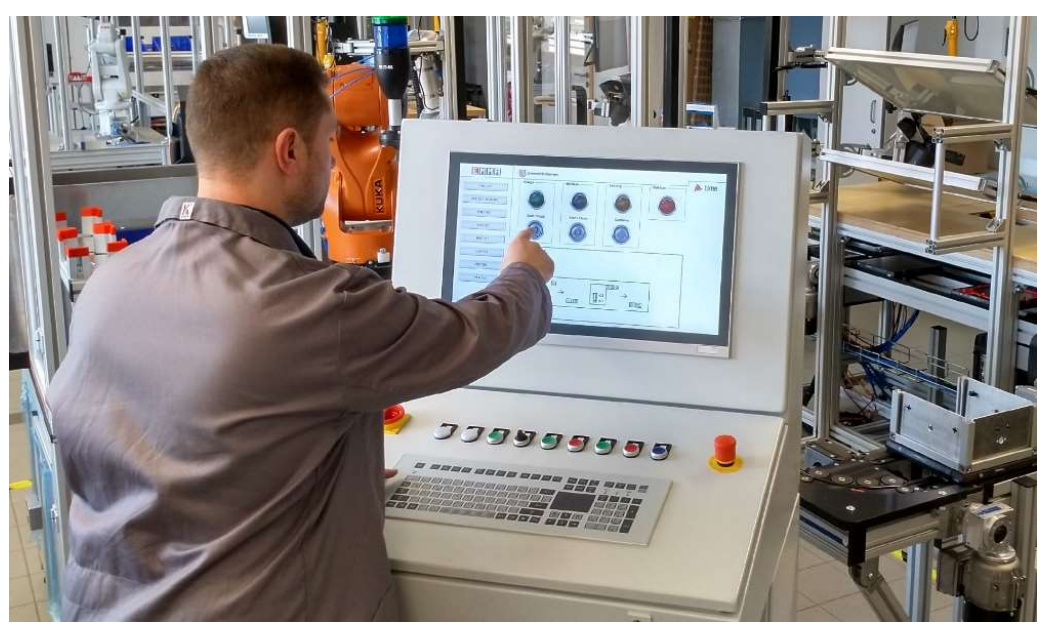
\includegraphics[width=\textwidth]{touchtaster1.png}
        \caption{固定式触摸屏}
        \label{fig:touchtaster1}
    \end{subfigure}
    \hfill
    \begin{subfigure}[b]{0.48\textwidth}
        \centering
        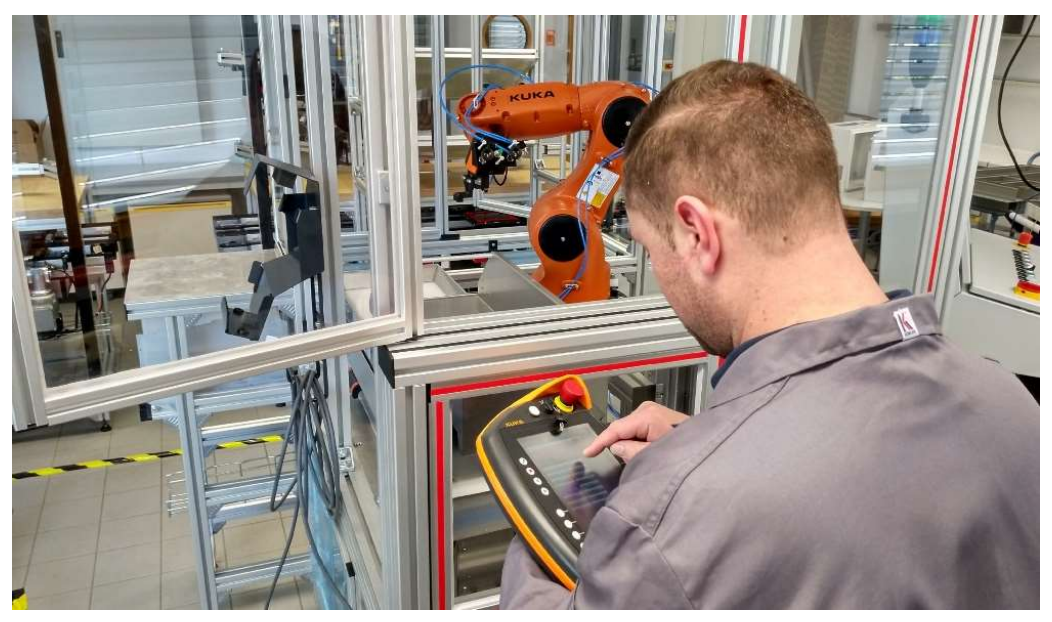
\includegraphics[width=\textwidth]{touchtaster2.png}
        \caption{移动式触摸屏}
        \label{fig:touchtaster2}
    \end{subfigure}
    \caption{触摸屏与机械按钮}
    \label{fig:touchtaster}
\end{figure}

用到的沟通渠道：光学通道（机器→人，负责状态展示）和触觉通道（人→机器，负责操作输入）。具体载体是触摸屏、机械按钮和开关、指示灯（有些和按钮做在一起），人这边用的是眼睛和手。

这个例子说明了最基础的人机交互方式。精简、可靠，关键安全功能坚持用机械按钮而不是纯触屏，也体现出讲义前面提到的技术层面干扰要尽量降到最低的设计思路。

\paragraph{数字化工位辅助系统（GeSA）}

数字化工位辅助系统用在手工装配工位，给工人提供数字化的辅助引导。如图 \ref{fig:gesa} 所示。它能自动识别装配进度，工人可以通过手势和二维码卡片来操作辅助系统，产品的中间检验和最终检验也是通过光学方式完成的。

\begin{figure}[htbp]
    \centering
    \begin{subfigure}[b]{0.44\textwidth}
        \centering
        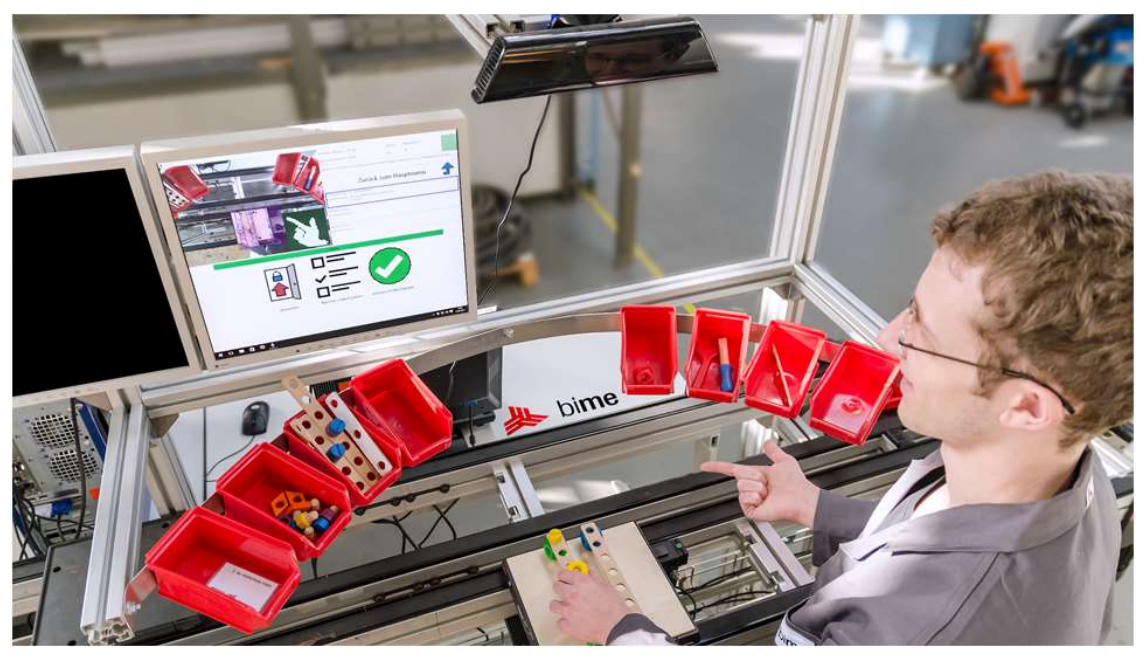
\includegraphics[width=\textwidth]{gesa1.png}
        \caption{GeSA的布置}
        \label{fig:gesa1}
    \end{subfigure}
    \hfill
    \begin{subfigure}[b]{0.49\textwidth}
        \centering
        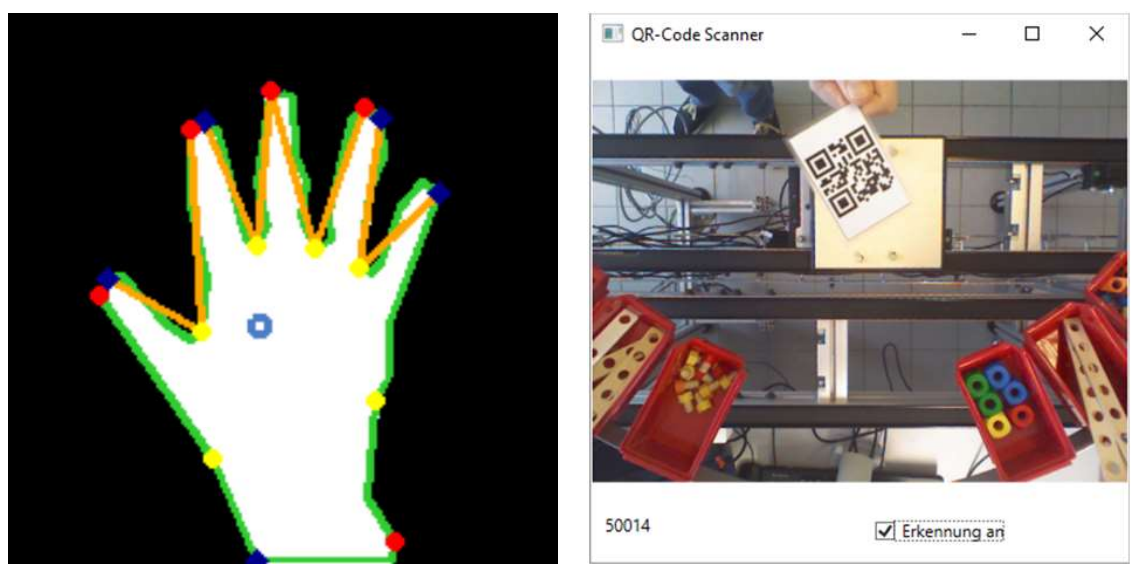
\includegraphics[width=\textwidth]{gesa2.png}
        \caption{操作界面}
        \label{fig:gesa2}
    \end{subfigure}
    \caption{GeSA}
    \label{fig:gesa}
\end{figure}

用到的沟通渠道是双向的光学通道：机器一侧靠深度摄像头和彩色摄像头识别，人这边用眼睛看显示屏、用手做手势，摄像头也能看到工件本身。

相比触摸屏与机械按钮，这里机器已经能主动看懂人的手势动作，是一个更主动、更智能的交互方式，呼应了 \ref{subsec:restriktoren} 小节提到的机器向人靠拢的适应策略。

\paragraph{装配辅助系统（Mona）}

装配辅助系统，如图 \ref{fig:mona} 所示，是面向大尺寸产品装配过程中的工人引导。系统靠骨骼追踪（Skelettracking）技术识别工人手臂姿态和手部位置，工作信息显示在显示屏上，工人通过两段式的手臂手势来操作系统。

\begin{figure}[htbp]
  \centering
  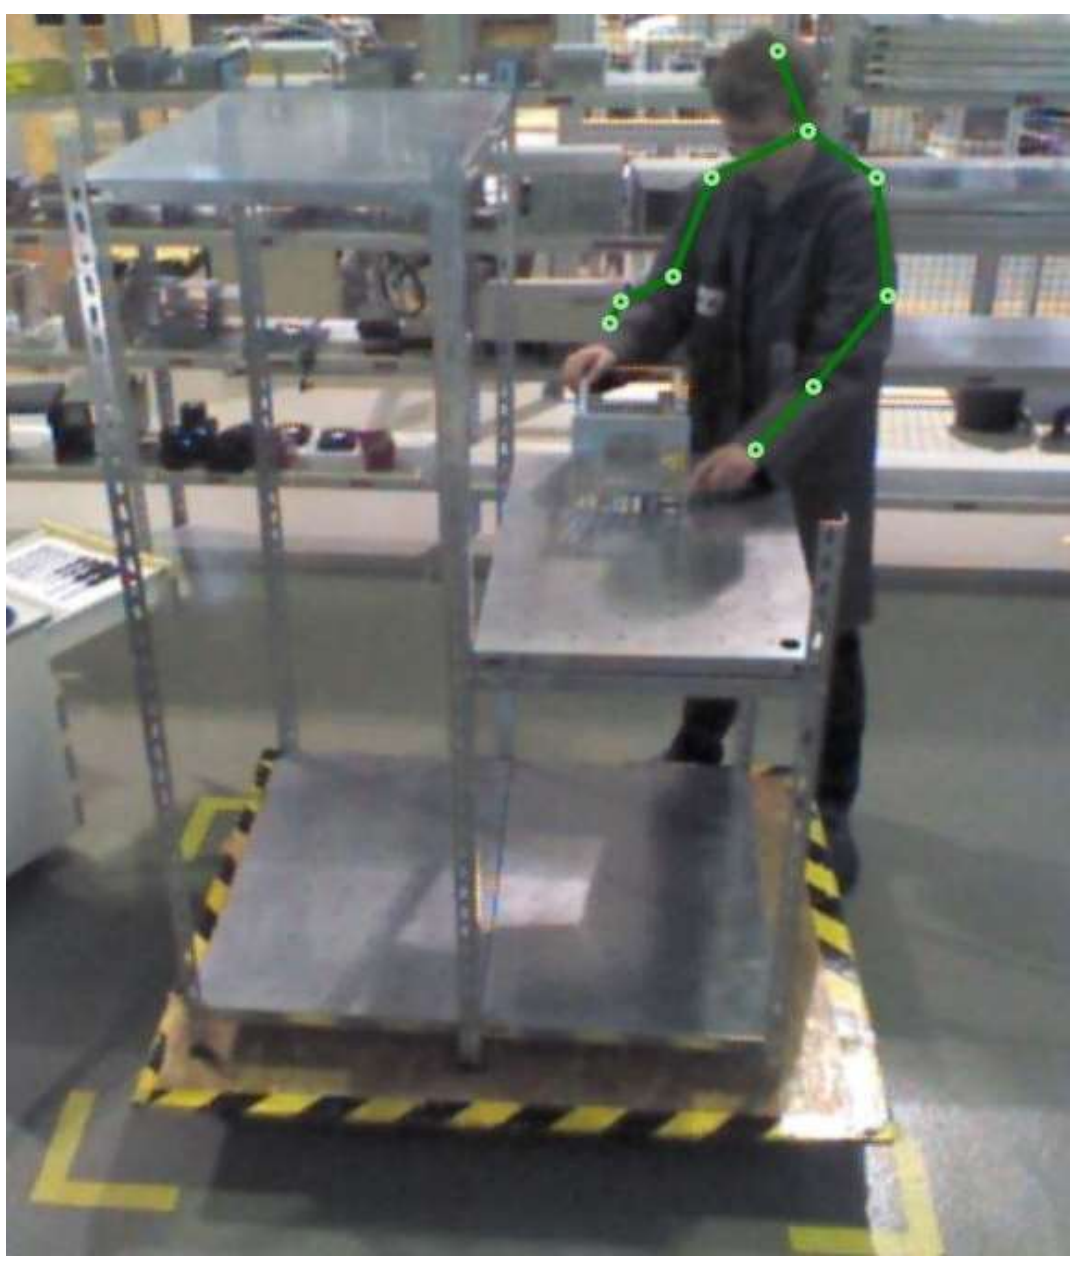
\includegraphics[width=0.4\textwidth]{mona.png}
  \caption{Mona}
  \label{fig:mona}
\end{figure}

沟通渠道同样是双向光学通道，用到深度摄像头、彩色摄像头、显示屏，人这边靠眼睛观察、手臂做动作。

这个案例和 GeSA 很像，但交互的身体部位从手扩展到了手臂，说明针对不同的装配场景（大件产品需要更大幅度的动作），交互方式也需要相应调整。

\paragraph{协作机器人的语音控制}

协作机器人用于协作装配场景。机器人按工序一步步地拿取和翻转装配对象，工人则负责抓取和安装零件，如图 \ref{fig:sprachsteuerung} 所示。工作说明和交互选项显示在屏幕上，工人可以用语音指令操作辅助系统，系统还能通过图像识别装配进度并进行产品检验。

\begin{figure}[htbp]
    \centering
    \begin{subfigure}[b]{0.48\textwidth}
        \centering
        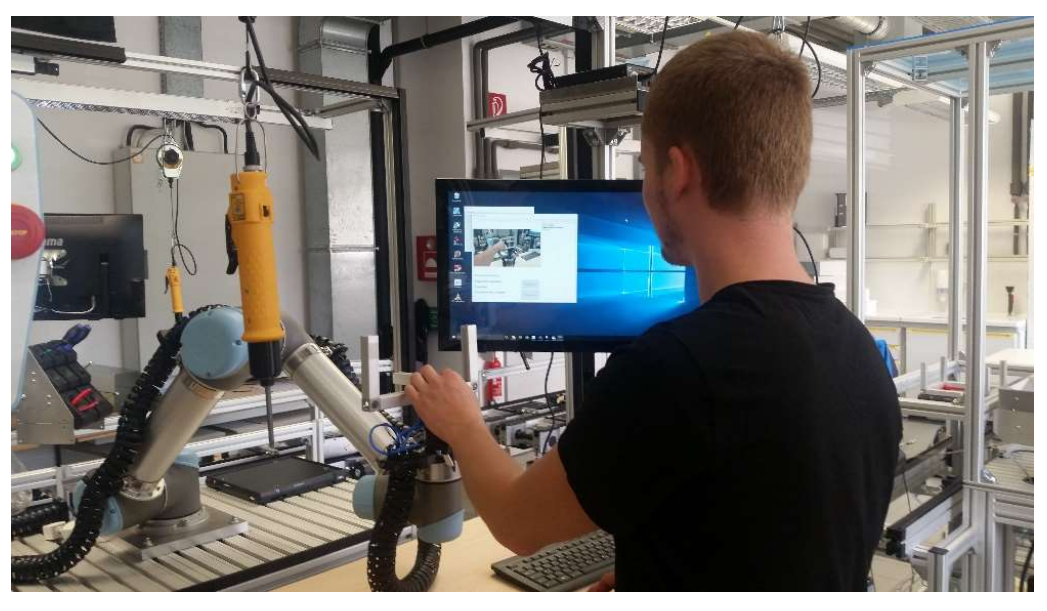
\includegraphics[width=\textwidth]{sprachsteuerung1.png}
        \caption{协作机器人的布置}
        \label{fig:sprachsteuerung1}
    \end{subfigure}
    \hfill
    \begin{subfigure}[b]{0.48\textwidth}
        \centering
        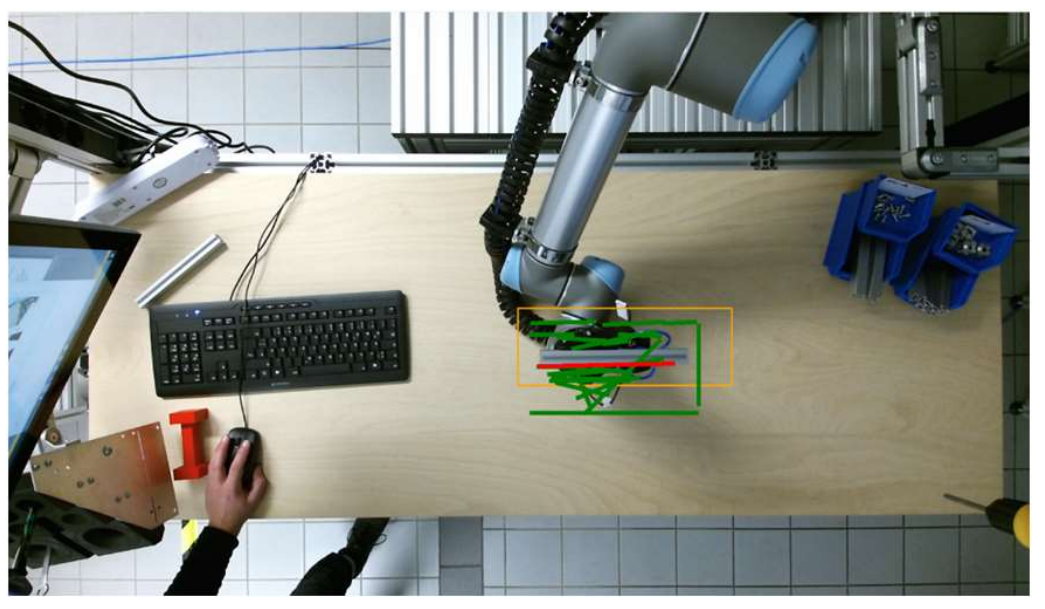
\includegraphics[width=\textwidth]{sprachsteuerung2.png}
        \caption{机器人视角}
        \label{fig:sprachsteuerung2}
    \end{subfigure}
    \caption{协作机器人}
    \label{fig:sprachsteuerung}
\end{figure}

这里首次出现了声学通道（人→机器，靠语音），同时叠加了双向光学通道（显示屏 + 彩色摄像头 + 深度摄像头，配合机器人动作展示状态）。用到的设备包括显示屏、机器人动作、麦克风阵列、深度摄像头,人这边用眼睛、声音。

这是六个案例里第一次用到说话这种更自然的沟通方式，也呼应 \ref{subsec:kommunikation} 小节提到的语言沟通。比起按钮和手势，语音交互对人来说更省心，但也对机器的语音识别能力提出了更高要求。

\paragraph{虚拟示教（KoKoMo）}

虚拟示教是对协作装配过程进行虚拟化呈现的系统。工作方式是先在虚拟环境中对机器人进行示教（Teach-in），再把学到的动作轨迹传输到真实设备上执行，生成的程序还能回传到仿真环境中验证。整个装配过程可以在 VR 和 AR 中先行测试。

\begin{figure}[htbp]
    \centering
    \begin{subfigure}[b]{0.56\textwidth}
        \centering
        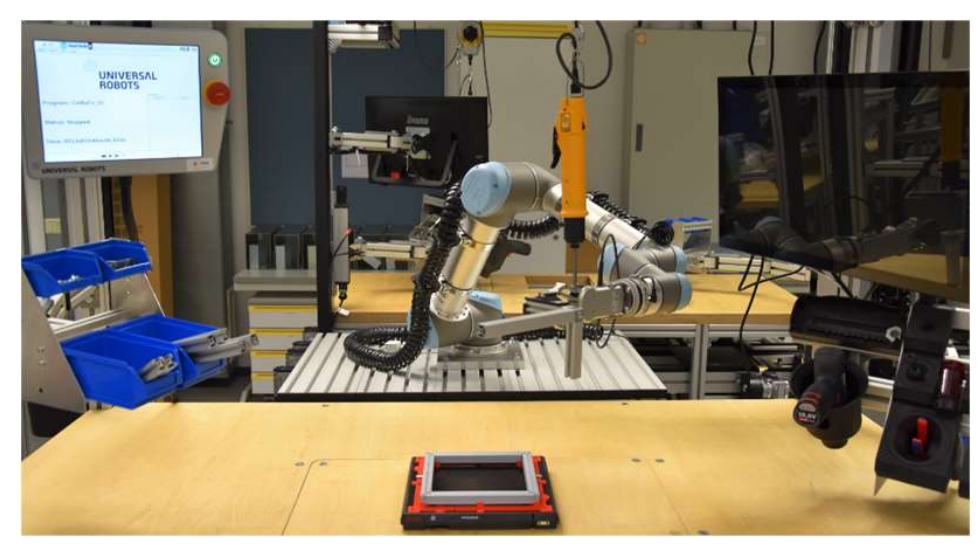
\includegraphics[width=\textwidth]{kokomo1.png}
        \caption{硬件视角}
        \label{fig:kokomo1}
    \end{subfigure}
    \hfill
    \begin{subfigure}[b]{0.40\textwidth}
        \centering
        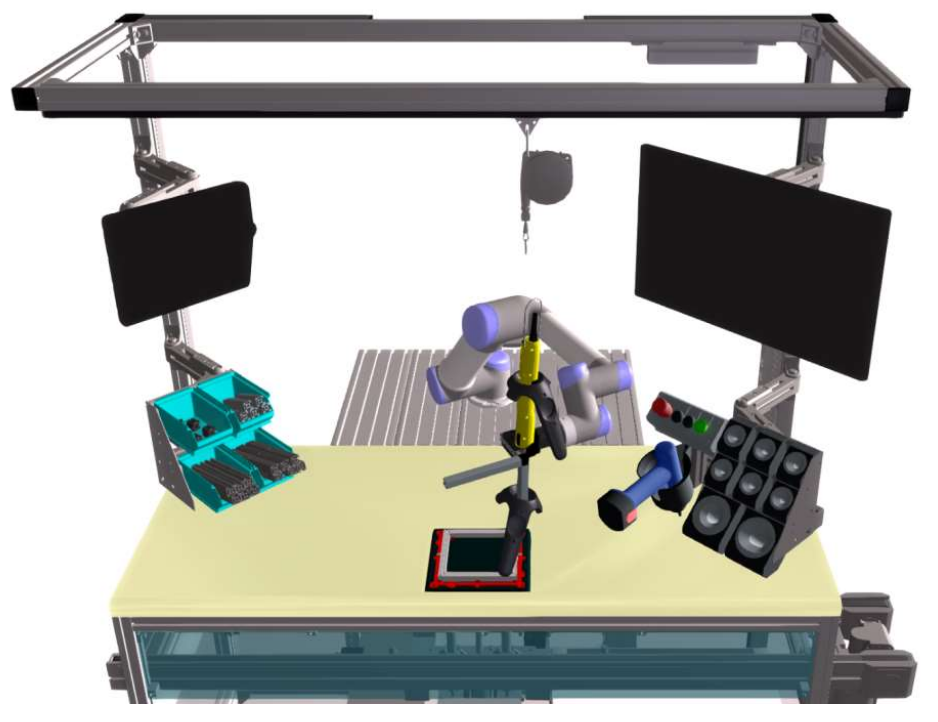
\includegraphics[width=\textwidth]{kokomo2.png}
        \caption{软件视角}
        \label{fig:kokomo2}
    \end{subfigure}
    \caption{虚拟示教（KoKoMo）}
    \label{fig:kokomo}
\end{figure}

这个案例用到了三种通道：双向光学通道（VR眼镜呈现画面）、双向触觉通道（VR控制器提供操作和反馈）、声学通道（耳机→人，输出提示音）。用到的设备有VR眼镜、VR控制器、耳机、红外传感器。

这是六个案例里交互渠道最丰富的一个，也正好对应 \ref{subsec:restriktoren} 小节提到的 Human in the Loop。人通过多种感官同时沉浸在虚拟环境里，跟真实设备的动作数据打通。

\paragraph{半机械化的机械手焊接}

工业焊接场景的应用：焊枪装在轻型机器人上，机器人架在带齿轮驱动的导轨上（相当于增加了第七轴以扩大作业范围），导轨通过磁铁固定在工件上；操作人员大致示教焊枪的轨迹点位和角度；车间里所有工人腰间都配有移动式急停按钮；通过专用摄像头和显示屏监控熔池状态；用操纵杆修正轨迹和焊枪角度。

沟通渠道是光学通道（机器→人，通过专用摄像头显示熔池状态）和触觉通道（人→机器，通过急停按钮和操纵杆操作）。人这边用眼睛看、手操作。

这个案例强调的是安全性：移动式急停按钮让车间里所有人都能随时中止流程，这也是工业场景下人机交互设计必须优先考虑的安全冗余。

\vspace{2em}

把六个案例放在一起看会发现几个明显的趋势：
\begin{itemize}
    \item 用到的沟通渠道从简单（案例一：触摸屏+按钮）逐步叠加更多通道（案例五：光学+触觉+声学三合一）
    \item 光学通道几乎是每个案例的标配，因为"看"是最直接、最容易实现双向反馈的方式
    \item 安全相关的功能（急停）无论系统多智能，始终倾向于用最可靠的机械式触觉交互来实现，而不是依赖摄像头识别或语音识别
    \item 案例越靠后，机器"理解"人的能力越强（从固定按钮，到识别手势，到语音理解，再到多通道融合的沉浸式交互），呼应第4节讲的"机器向人靠拢"的发展方向
\end{itemize}




\section{工业4.0下人的角色}

\subsection{工业4.0下人的角色}

在一个到处都是自动化、机器人、传感器的工业4.0世界里，人到底还有没有位置？答案其实是肯定的，我们将从概念、身体负荷到具体案例,一步步说明为什么人依然重要,以及技术应该怎么帮人。

在工业4.0之前,90年代很流行一个叫CIM(计算机集成制造)的理念,核心思路是尽量把人从生产线上“计算机化”掉。理想状态就是一座\emph{不需要人的工厂}，\emph{计算机占据主导地位}，人只是生产中次要的角色。工业4.0则反过来了。\emph{人被重新放回中心位置}，角色变成了问题解决者、\emph{经验和知识的载体}、做决策的人。\emph{生产这一侧则交给自动化}、包容性设计、人体增强、各种辅助系统，以及能察言观色、根据情境自动调整的交互界面去承担。

要理解为什么需要辅助系统,得先看清人在车间里实际承受的身体负荷。不同的工作类型会集中损耗身体的不同部位：负重搬运主要伤腰椎、肩膀、髋关节和膝盖；头顶作业主要伤颈椎、肩膀、胸椎和腰椎；精密装配则容易造成肩膀、颈部、手腕的劳损，还需要持续的注意力。

工业4.0里人的角色发生了根本转变，\emph{从CIM时代“能不用人就不用人”,变成了“人是核心,技术要配合人”；再用身体负荷的分析，论证辅助系统存在的必要性；然后用一堆真实案例证明这些技术已经在各行各业落地；最后指出目前这个领域还缺一套系统的分类方法。}

\subsection{人机分工}

四次工业革命，每一次都会重新定义人需要具备什么能力。我们把这些能力归纳成六个能力领域：
\begin{itemize}
    \item 身体负荷承受能力(physische Beanspruchung)
    \item 情绪负荷承受能力(emotionale Beanspruchung)
    \item 心理/脑力负荷承受能力(mentale Beanspruchung)
    \item 专业能力(Fachkompetenz)
    \item 社会能力(Sozialkompetenz)
    \item 个性能力(Persönlichkeitskompetenz)
\end{itemize}
也就是说，工业4.0对人的要求已经不只是“体力好、手艺熟”,而是身体、心理、专业、社交、个性多方面综合的能力。

既然要谈谁该做什么,就得先弄清楚人和机器分别擅长什么。人的优势集中在认知能力(Kognition)、感知运动协调能力(Sensomotorik)、学习能力(Lernfähigkeit)。简单来说人擅长的就是灵活应变、理解情境、不断学习。

技术系统的优势集中在:精度(Genauigkeit)、速度(Geschwindigkeit)、可靠性(Zuverlässigkeit)、抗负荷能力(Belastbarkeit,包括脑力和体力两方面)、耐力和抗疲劳/抗分心能力 (Ausdauer/~Ermüdungsanfälligkeit/Konzentrationsfähigkeit)，所以机器擅长的是稳定、精确、不知疲倦地重复。

既然人和机器的强项在很多地方是相反但互补的，那就应该通过合理搭配，用技术系统、工具和功能去补上人的短板，同时保留人在认知和灵活应变上的优势，而不是简单地用机器把人整个替换掉。这就是人机智能混合(intelligente Hybridisierung von Mensch und Technik)。

\paragraph{任务分配的阶段(Stufen der Aufgabenverteilung)}

如图 \ref{fig:stufenaufgabenverteilung} 所示，从Stufe 0(完全人工)到Stufe 4(完全自动化)。我们把一项工作拆成四个维度,看每个维度在不同阶段里是由人还是由机器主导:
\begin{itemize}
    \item 过程主导权(Prozesshoheit):谁来决定整个流程怎么走
    \item 监控(Überwachung):谁来盯着任务执行得对不对
    \item 感知(Sensorik):谁来获取环境和任务状态的信息
    \item 施力(Kraftaufbringung):谁来实际出力完成动作
\end{itemize}

\begin{figure}[htbp]
  \centering
  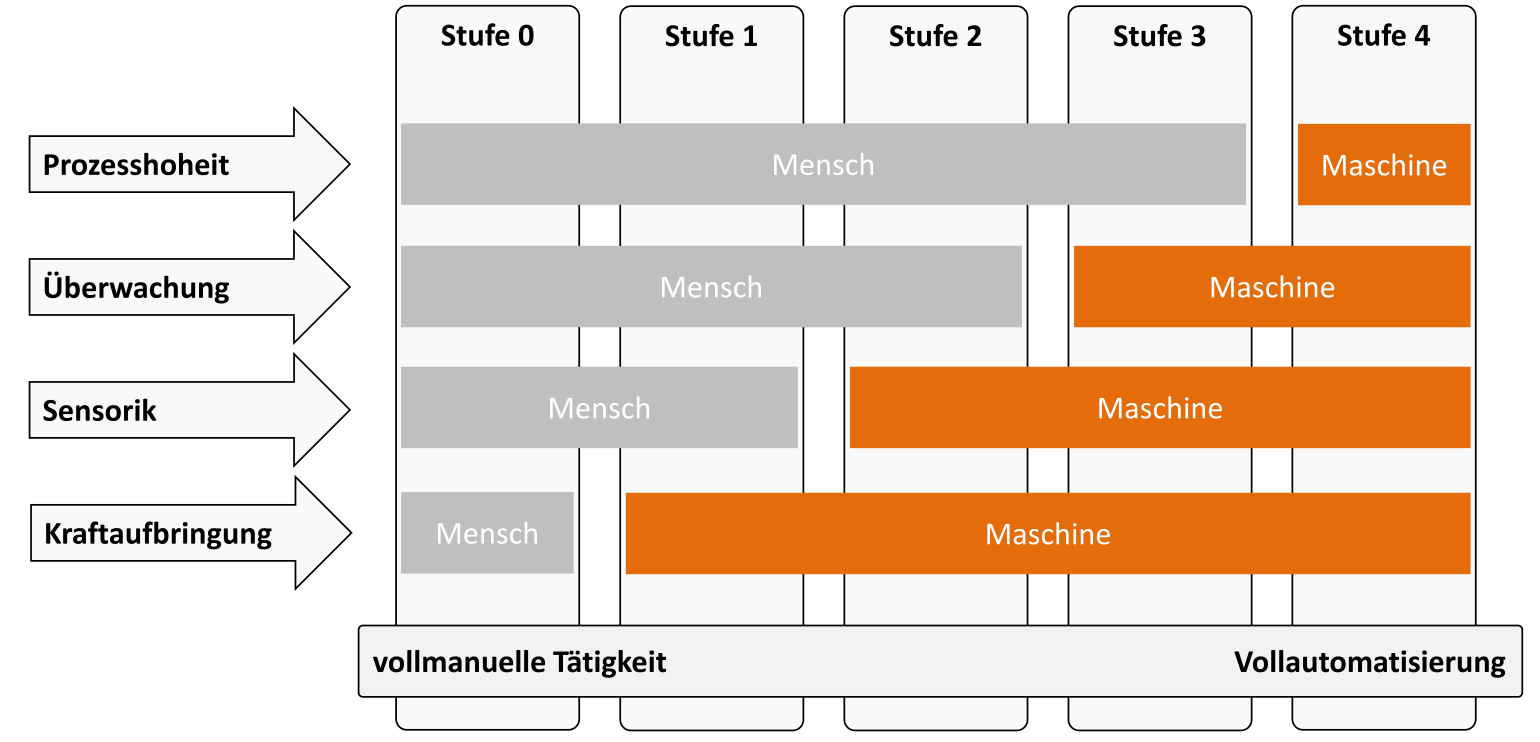
\includegraphics[width=0.8\textwidth]{stufenaufgabenverteilung.png}
  \caption{任务分配的阶段}
  \label{fig:stufenaufgabenverteilung}
\end{figure}

有意思的是,这四个维度并不是同步从人切换到机器的,而是有先后顺序:最先交给机器的是施力(比如用电动工具代替纯手力),然后是感知(比如用传感器代替人眼观察),接着是监控(比如系统自动报警代替人工巡检),最后才轮到过程主导权(也就是让机器自己决定怎么做),这也是自动化程度最高、最难实现的一步。两端分别对应完全人工作业(vollmanuelle Tätigkeit)和完全自动化(Vollautomatisierung),中间则是各种程度不一的人机协作组合。

\subsection{技术支持系统}

人和人是不一样的,所以支持系统不能是一刀切的,必须足够灵活。

造成个体差异的因素被分成了两类。一类是人本身的特征:年龄、性别、既往经验、认知与注意力水平、动作模式与行为习惯。另一类是可以量化的身体参数:人体测量数据、力量、柔韧性、心肺功能/耐力、既往损伤史。这些因素叠加起来,意味着同一套支持系统,对不同的人可能效果完全不同。这也是后面模块化设计思路的起点。

各个活动场景需要的支持方式不一样，有的需要力的转向,有的需要力的转向加放大,有的需要单纯的力量放大,还有的需要稳定与质量保证。所以支持系统不应该是一个笼统的概念,而是要针对具体场景设计具体功能。

我们用三个维度来判断一个人机协作属于哪一种形式：
\begin{itemize}
    \item \emph{时空关系}:人和机器是分开工作、共处一地但独立、分布式协作,还是完全融合?
    \item \emph{耦合形式}:是辅助还是更紧密的耦合?
    \item \emph{控制权归属}:由人还是由技术主导,而且这种主导是暂时性的还是永久性的?
\end{itemize}
这三个维度组合起来,划分出三条典型路径,分别对应不同紧密程度的人机协作关系。这也是理解后面各种具体支持系统"到底算哪一类"的一个坐标系。

一个技术系统要被称为支持系统,必须同时满足四个条件:
\begin{enumerate}
    \item 它能帮助人完成任务,而不是完全或部分地替代人
    \item 执行的主导权仍然掌握在人手里(由操作者给出目标值,而不是系统强制规定)
    \item 人是这个系统的操作者
    \item 系统本身不会对操作者或第三方造成危险
\end{enumerate}

除了减轻当下的身体负荷，引入支持系统还有三层更长远的理由：
\begin{itemize}
    \item \emph{补偿机能衰退} (Kompensation von Funktionseinbußen)：人的体力、柔韧性、视力、反应速度都会随年龄增长而下降，既往损伤也会留下永久性的能力缺口。支持系统可以把这部分损失的能力补回来，让因年龄或身体条件受限的人依然能胜任原本的工作岗位，而不是被迫调岗或离开生产线。
    \item \emph{更长久地保持健康} (längerer Erhalt der Gesundheit)：负重搬运、头顶作业、精密装配这类工作的损伤是长期累积的，等到肌肉骨骼疾病显现时往往已经不可逆。支持系统的作用是提前把负荷峰值压下去，把作用在腰椎、肩关节上的力转移到设备上，从而延长人的职业寿命，降低企业的病假成本和工伤风险。
    \item \emph{技术接受度与可接受性} (Technikakzeptanz und -akzeptabilität)：一套系统再先进，员工不愿意用也等于零。接受度指的是使用者主观上愿不愿意用——设备是否舒适、是否拖慢节奏、是否让人觉得被监视；可接受性则是更外部的判断，即这套系统在伦理、法律和社会层面是否应当被接受——数据采集的边界在哪里、会不会造成新的能力依赖。只有两者同时成立，支持系统才可能真正落地。
\end{itemize}

\paragraph{支持系统的模块化设计思路}

支持系统必须因人而异、因任务而异,\emph{为了实现这种灵活性}，我们把支持系统拆成几类可以自由组合的模块。

首先是基础参数模块,涵盖人体\emph{测量数据、负荷、能力、技能、复杂度、持续时间,用于描述这个人和这项任务的具体需求}。比如在头顶高度用重工具装配时,需要弯曲/伸展/旋转功能加抬起/放下/保持功能,再配合膝部支撑等具体模块组合出一套解决方案。

其次是人机接口模块,按感知渠道分成触觉、视觉、听觉三类。

然后是传感器模块,分成两类接口:物理接口(比如EMG肌电传感器、一维/三维力传感器、力敏薄膜传感器、压力传感器)和认知接口(比如摄像系统、眼动追踪、脑电EEG传感器、语音识别)。

最后是控制与调节模块,同样分物理和认知两类支持:物理支持包括力控制(按位置调节或由使用者主动调节)和意图识别(无意识/自动化控制,结合EMG传感器和动作识别);认知支持包括防错机制(Poka-Yoke)、工作现场监控(比如用摄像系统监控作业、偏差提醒)、轨迹/抓取路径给定(从CAD数据或系统学习中获得),以及反馈功能(声音、视觉、触觉多种形式提示偏差)。

这一整套模块化思路的意义在于与其为每个人、每个任务单独设计一套系统,不如把常用的功能拆成标准化的模块,按需组合。

\paragraph{支持也是一把双刃剑}

支持系统并不是越多越好, 而是有代价的。

好处：
\begin{itemize}
    \item \emph{}身体减负 (körperliche Entlastung)：外骨骼、力平衡装置把原本压在腰椎和肩关节上的负荷转移到设备上, 肌肉骨骼疾病明显减少。
    \item \emph{}质量提升 (Steigerung der Qualität)：防错机制、轨迹给定和实时反馈让作业结果更稳定,出错次数下降。
    \item \emph{}生产率提升 (Steigerung der Produktivität)：力量放大和辅助定位缩短了单件工时, 人还能获得超能力式的力量加成。
    \item \emph{}动作追踪(Bewegungsverfolgung)：支持系统本身就装有力传感器、EMG 传感器或摄像系统, 这些数据顺带就能用于工效学评估、作业分析和长期健康监测, 不需要额外部署一套采集系统。
\end{itemize}

代价：
\begin{itemize}
    \item \emph{接受度问题} (Akzeptanzprobleme)：设备穿戴不舒服、拖慢了原本的作业节奏、或者让员工觉得自己被监视, 都会导致系统被闲置。
    \item \emph{系统设计错误}(falsche Systemauslegung)：支持力给得不对、支撑点选得不对, 不仅达不到减负效果,反而可能把负荷转移到别的部位, 制造出新的劳损。
    \item \emph{岗位轮换被取消}(Aussetzen der Job-Rotation)：一旦某个工位配了专用支持设备, 企业往往倾向于让固定的人长期留在这个工位上, 原本靠轮岗实现的负荷分散就没有了, 单一部位的累积负荷反而上升。
    \item \emph{能力退化}：长期依赖支持设备可能导致肌肉退化、身体能力下降; 认知层面同理, 辅助给得太多会让人逐渐丧失原本具备的判断力。所以支持的度要拿捏得当, 这件事从长期看非常重要。支持不足解决不了问题,
\end{itemize}


% !TeX root = main.tex
\section{传感器系统}

\subsection{机器人传感器}

\subsubsection{传感器的定义、任务与分类}

工业机器人本身按照预先编好的程序动作，理论上并不需要感知外界。但现实生产中，很多情况让机器人必须依靠传感器才能正常工作。典型情形有：
\begin{itemize}
    \item 工件有时\textbf{无法有序摆放}，比如批量很小、型号种类多、工件本身很大，或者工件形状复杂，这些都让机器人无法按固定坐标去抓取。
    \item \textbf{工件和工件夹具的公差过大}，比如锻造和炉子作业中工件会因受热膨胀，铸件和压铸件边缘还常有毛刺，这些偏差都需要传感器去补偿。
    \item 工件\textbf{被连续移动的传送装置搬运}的场景，比如悬挂输送线或传送带，这时机器人需要具备传送带跟踪的能力，让机械臂的运动和不断移动的工件保持同步，喷漆、表面处理等工序中工件往往还会摆动或者悬挂得不太精确，进一步增加了难度。
    \item 工件的\textbf{转向角未知}，比如装配一个旋转部件时，机器人得先识别出它当前处于什么角度。
    \item \textbf{工件本身柔软易变形}，比如电缆、软管、电线、纺织品这类东西，形状不固定，抓取和装配都更依赖实时感知。
    \item 机械式的硬自动化容易出故障，用传感器可以及时发现并灵活应对这些异常，从而减少人工质检和人工干预的次数
    \item \textbf{加工精度要求超过了机器人本身能达到的绝对精度}，比如精密滚动轴承的装配、飞机侧翼的钻孔、大型机器人给飞机做清洗，这些场合机器人自身的定位精度不够用，必须靠传感器来补足。
    \item \textbf{机器人编程本身很繁琐}，这时可以借助传感器自动生成运动轨迹，或者先粗略编好轨迹，再叠加传感器做精细修正。
\end{itemize}

\textbf{传感器是一种测量值拾取器，它获取物体的属性、状态和过程信息，并把最重要的输入信号转换成合适的输出信号。}人类的感知能力常被当作衡量机器人传感能力的标杆，在一些专门场合，机器人传感器的表现甚至已经超过了人类。

传感器在机器人上除了做物理量到电信号的转换之外，更重要的作用是承担较高层次的信息处理和解释工作。具体来说，它要帮机器人应对以下几方面的精度需求：机器人本体运动学的精度、机器人外围设备的精度、工件本身的精度，以及作业空间里不断变化的环境条件。

按照传感器安装的位置和作用对象，可以分为\textbf{内部传感器}和\textbf{外部传感器}两类。内部传感器让\textbf{机器人感知自己的内部状态}，比如速度、位置、力和力矩；外部传感器则\textbf{负责获取机器人所处环境的信息}，包括感知被操作对象和周围环境的状态、识别和判断工件的性质、测量各种物理量，以及分析周围场景。

外部传感器按照工作原理又可以分为接触式和非接触式两大类。接触式传感器包括触觉类（如开关、触点矩阵、面式开关）和力/力矩类（用于测量夹持力、力和力矩）；非接触式传感器则包括视频光学类（二维图像处理、灰度处理、三维立体视觉）、感应/电容/磁性类（接近开关、测距仪、焊缝识别）、光学测距类（光电门、光切法、一维测距、二维/三维扫描仪），以及超声波类（接近开关、测距仪、扫描仪）。整个传感器分类结构如图 \ref{fig:sensorstruktur} 所示。

\begin{figure}[htbp]
  \centering
  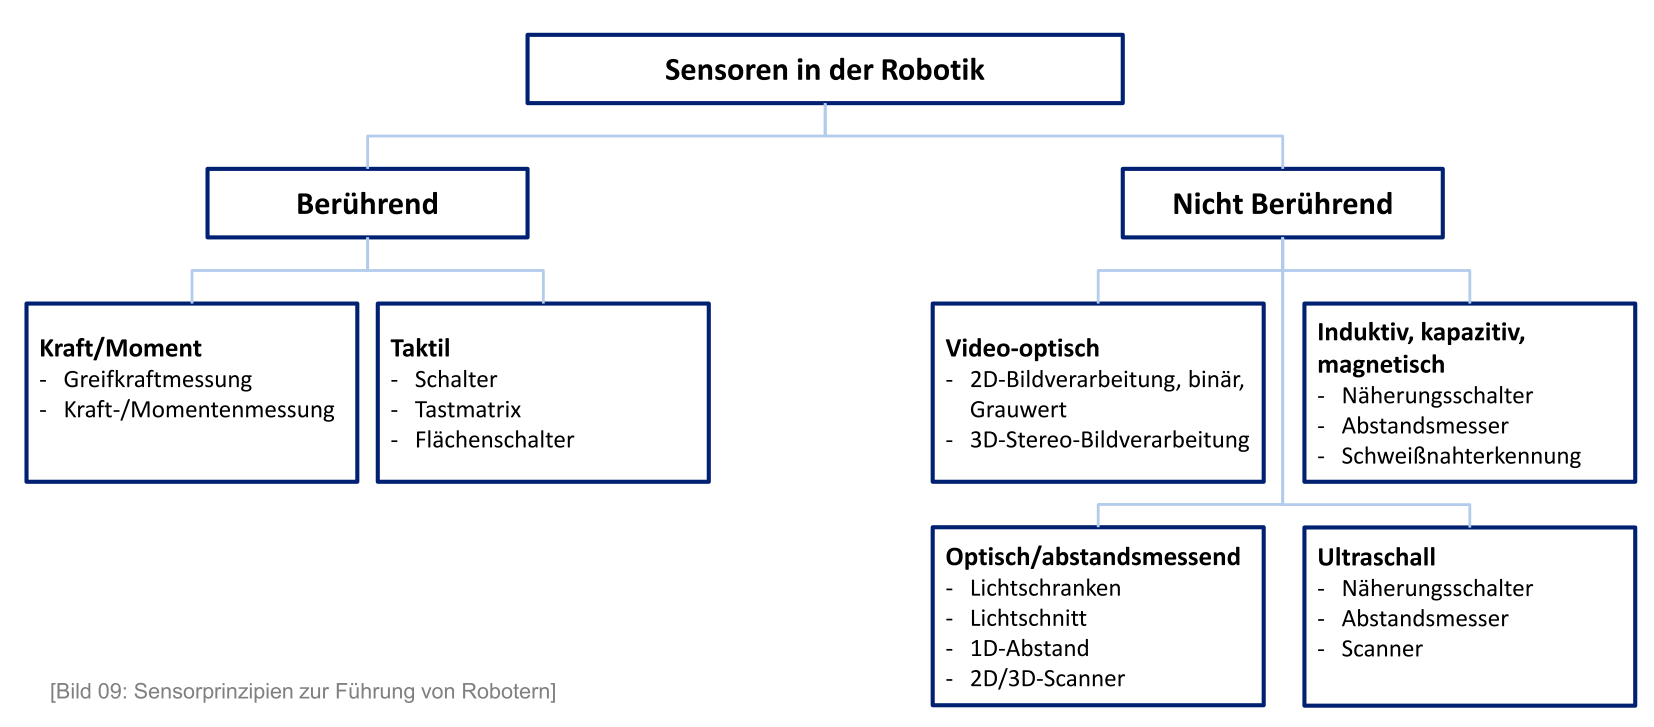
\includegraphics[width=0.9\textwidth]{sensorstruktur.png}
  \caption{传感器分类结构}
  \label{fig:sensorstruktur}
\end{figure}

\subsubsection{接触式传感器}

触觉传感器通过直接接触物体来获取环境信息，最常见的例子是集成在夹爪里的二值开关，抓取动作完成后它会给出零件已成功抓取的信号，一旦抓取失败就触发重试或者错误处理流程；另外像安全防护用的开关垫也属于这一类。触觉传感器还有一种典型应用是焊枪嘴：把喷嘴做成可以小幅度摆动的结构，内部装两个微动开关，喷嘴沿焊枪轴线方向可以偏移最多6毫米，垂直方向最多25毫米，一旦喷嘴偏移，微动开关就被触发，从而在焊接开始前探测出焊缝的起点和终点，如果焊接过程中发生碰撞，还能立即中断焊接。这种触觉传感器的搜索速度大约是每分钟2米，搜索精度大约是正负0.2毫米。除了这种摆动式喷嘴，实际中还会用球形触头、圆盘形触头，以及专门用于内角焊缝的角部触头。触觉传感器的优点是成本低、结构简单，而且不怕焊接过程中的光学干扰；缺点则是容易磨损、测量精度有限，也容易被污染影响。

触觉传感器还有一类是面状分布的触觉阵列，利用不同的物理转换原理来生成矩阵式的触觉信息，讲义举了压电PVDF薄膜的例子：这是一种带有明显压电效应的热塑性塑料薄膜，厚度大约在10到100微米之间，薄膜两面镀铝，通过局部蚀刻的方式在薄膜上做出矩阵式的感应点，只有上下两面之间仍保持电极化关系的区域才会起作用。

图 \ref{fig:beruhrendesensor} 中所示的\textbf{力/力矩传感器}相当于给了机器人触觉，把这种传感器装进机器人后，可以实现\textbf{精密零件的装配定位、自动化装配作业，以及由机器人自主完成的质量检测}。安装位置通常在机器人手腕和末端执行器之间，或者直接装在末端执行器内部，也可以集成到工件夹具中。这类传感器内部一般带有数字信号处理器，负责采集和过滤应变信号、计算出对应的力和力矩数值，再通过通信接口把结果传出去。讲义还展示了一种典型结构：两层叠放的改造过的辐条轮结构，工作原理是先把受到的力和力矩转化成弹性辐条的微小长度变化，再通过应变片把这种变化转成电信号，最后借助一个所谓的"解耦矩阵"，从各个传感元件的信号中解算出力和力矩的各个分量，这本质上是求解一个和具体结构相关的线性方程组。这类传感器普遍存在的问题是信号里常常叠加着振荡成分，影响信号质量，虽然可以通过后处理和滤波来改善，但往往会牺牲一部分信号的动态响应速度。

\begin{figure}[htbp]
  \centering
  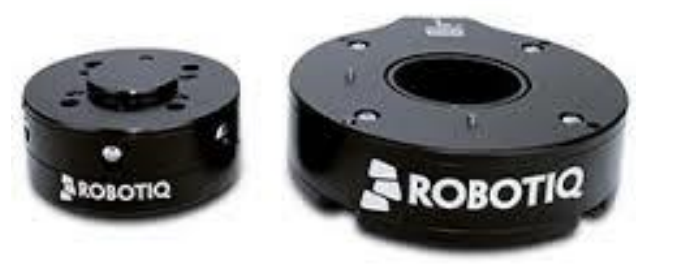
\includegraphics[width=0.4\textwidth]{beruhrendesensor.png}
  \caption{力/力矩传感器}
  \label{fig:beruhrendesensor}
\end{figure}

\subsubsection{非接触式传感器}

视频光学传感器的工作方式是先拍摄工件场景的图像，再通过计算机做图像处理，从而判断物体的种类、数量和位置。一套典型的图像处理系统通常需要先经历一个示教阶段：把要识别的物体以不同姿态呈现给系统，从中总结出效果较好的预处理、物体分割和特征计算算法，尽量用少而准确的特征来描述物体，图像处理软件在整个系统里是核心环节，针对不同任务通常会配有模块化的软件包。

二值图像处理系统对光照条件的变化非常敏感，很多情况下需要配合专门的光照控制装置；灰度图像处理系统的可靠性则明显更好。常见的照明方式包括透射光和反射光两种：透射光用来呈现透明物体的内部结构，或者拍出不透明物体的轮廓（需要有透明的衬底）；反射光则用来突出物体的表面结构，根据入射角的不同又可以分为漫反射光和定向反射光。漫反射光照明比较均匀，物体转动或者在承载面上平移时反射效果变化不大，因此常用于工件识别；定向反射光则能更好地呈现工件表面的纹理结构。为了消除运动模糊，有时还会用与生产节拍同步的闪光（多为红外光）。反射光还可以做成局部投影的形式，比如点状、线状或条纹状的图案，甚至是不规则或者面编码的图案投射到物体表面，这样就能实现三维形状的采集——投出的线条越细，说明测量距离越远，这种照明技术被称为光切法。

视频光学传感器另一个重要应用方向是物体识别，如图 \ref{fig:nichtberuhrendesensor} 所示。要让生产过程高效运转，一个基本前提是能在最短时间内准确无误地识别出物体，这就是自动识别（AutoID）技术要解决的问题。对一套自动识别系统的要求包括：在给定条件下保证足够高的读取可靠性、满足输送环节所需的读取速度、能够生成足够多样的识别标记、读取距离能够根据实际情况调整、与供应链上其他环节保持兼容，同时还要控制识别系统和相关设备的成本。识别所依据的特征既可以是物体本身固有的属性，比如颜色、重量、体积、材质、长宽高、包装材料、温度等，通过组合多个特征进行分类，进而完成物体的分拣；也可以是人工添加的识别标记，比如各种条码、二维码（QR码、矩阵码等），这些标识符可以存储在纸张、磁卡、打孔纸带或者RFID标签等不同载体上，再通过条码扫描器、二维相机等专门的读取设备来读取。另外还有一种识别技术是RFID（射频识别），它通过感应或者电磁波，在不需要直接光学接触的情况下就能非接触地采集和传输二进制编码的数据。

\begin{figure}[htbp]
  \centering
  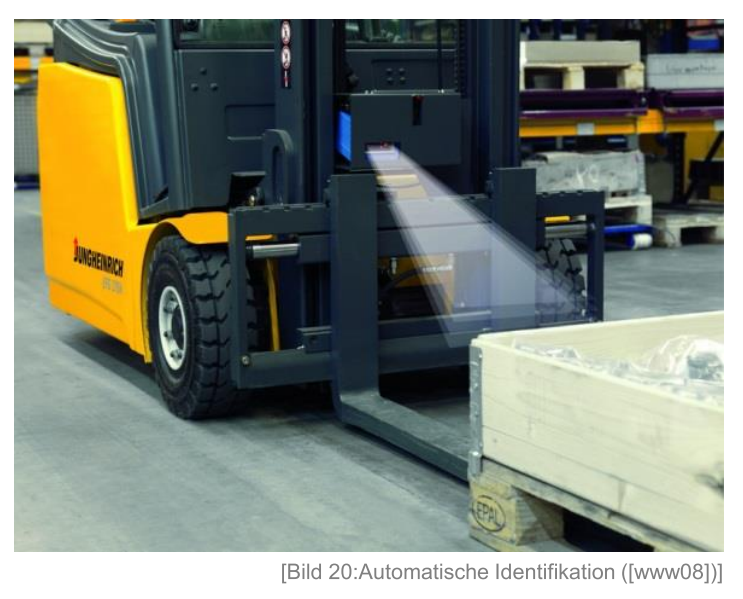
\includegraphics[width=0.4\textwidth]{nichtberuhrendesensor.png}
  \caption{用于物体识别的视频光学传感器}
  \label{fig:nichtberuhrendesensor}
\end{figure}

感应式传感器大多利用涡流原理工作：一个开口的壳形磁芯是LC振荡电路的一部分，用来产生高频振荡。一旦有导电物体进入这个向外发散的磁场，物体内部就会产生涡流，这个涡流会从振荡回路里"抽走"一部分能量，导致振荡幅度下降，这个变化会被电子电路检测出来，再通过和一个固定阈值比较，就可以得到一个距离信号。常见的环形线圈感应器的工作范围大约是线圈半径的0.01到1倍。这种测量原理在机器人领域常用于距离极限开关、位移传感器和脉冲发生器。感应式传感器在实际应用中主要用于焊接机器人的焊缝跟踪，尤其适合对接焊缝和搭接焊缝这类形状规则的焊缝，因为结构简单、成本较低，常被用在焊缝起点检测、跟踪直线或轻微弯曲焊缝这类相对简单的任务上。但如果焊缝弯曲程度比较大，感应式传感器一般就不适用了（磁场较强时传感器需要提前探测，容易受影响），另外焊接飞溅和夹具也会产生歧义信号，进一步限制了它的使用场景。

\subsection{面向工业4.0数字化的3D测量技术}

数字化的本质是\textbf{把物体表面用离散化的方式重建出来}，\textbf{测量和检测数据能反映产品和加工过程的状态是质量保障的基础}，而数据所包含的信息量高低很大程度上取决于所用的传感系统。

激光类3D测量系统（全站仪、激光跟踪仪、激光扫描仪）在原理上都是\textbf{极坐标测量}：分别测出到目标点的距离和两个方向角，再合成为三维坐标。

距离测量最基本的三种方法是脉冲飞行时间法、相位比较法和三角测量法。
\begin{itemize}
    \item 脉冲飞行时间法通过测量激光脉冲往返的飞行时间来计算距离，是激光系统最主要的测距方式；
    \item 相位比较法通过观测和分析持续发射的载波信号的相位移完成测距，部分激光设备也采用这种方式，通常精度更高但量程受限；
    \item 三角测量法则是在固定基线的前提下，通过观测角度的变化来推算距离。
\end{itemize}
角度测量方面，水平角和垂直角由\textbf{角度编码器（Winkelencoder）}测得：既可以采用固定刻度盘的静态方法（编码轨迹法、增量法、插值法），也可以采用旋转刻度盘的动态方法（把方向测量转化为时间测量），此外还有不需要刻度盘的激光陀螺仪。

需要注意这两类系统在原理上的分工：激光系统依靠"测距 + 测角"直接得到点的极坐标，而相机系统和混合系统（摄影测量、条纹光投影）则依靠\textbf{三角测量法}获取深度信息——通过已知基线上的两个（或多个）视角对同一物点的交会来反算其空间坐标。

在极坐标式、逐点测量的系统中，比较典型的代表是全站仪和激光跟踪仪。全站仪的测程可以达到3500米，精度约为0.6毫米加上百万分之一的比例误差，主要用于对超大型结构做中等精度要求的测量；激光跟踪仪的测量体积可达120米，精度约为15微米再加上每米6微米的比例误差，适合对大型结构做非常高精度的测量。这类设备的典型应用包括船舶建造中的尺寸质量检验（比如在船体分段合拢过程中逐点检查节点位置、给出分段与理论位置的偏差以便进一步校正定位），以及风电叶片模型的几何质量控制（因为测量体积大而公差要求又很严格，对精度的要求非常高）。

面测量系统大多基于激光扫描仪，按测量体积和使用方式大致可以分为三类：手持式扫描仪测量体积较小，适合手动扫描自由曲面，采样速率可达每秒50万个点；近距离扫描仪测量体积中等，一般固定放置进行扫描，对固定场景的测量精度较高；地面激光扫描仪测量体积最大，以栅格方式扫描表面并同时记录反射光的强度，采样速率可以超过每秒100万个点，测量距离可以达到160米。地面激光扫描的典型应用包括船舶建造中对现状的数字化（用来指导后续的刮腻子等工序、提高预制加工的比例），以及对建筑毛坯结构的采集（作为设计幕墙构件、并根据实际轮廓做适配调整的依据）。

光学测量系统在结构上一般包含图像采集、图像传输、图像预处理和图像处理四个环节。图像采集依靠CCD或CMOS传感器完成矩阵式的离散采样和数字化；图像传输通过DVI、HDMI、WLAN等标准化信号输出；图像预处理运用各种数值方法改善图像质量、降低噪声、提高对比度；图像处理则负责自动提取特征或者做模式识别。其中一个重要的技术分支是摄影测量学，主要用于对静态场景做高精度测量：通过CCD矩阵完成图像测量，得到图像坐标；再通过"图像定向"，借助已知的定向点（比例尺）及其图像坐标，结合相机参数的近似值，反推出拍摄瞬间相机在空间物体坐标系中的位置和姿态；有了至少两张图像的图像坐标、至少四个定向点的物体坐标，再加上相机参数的近似值，就可以通过"前方交会"（多像三角测量）反算出物体上各点的坐标；最后还会通过"光束法平差"，把测量误差均匀分摊到所有参与计算的图像上，以提高整体精度。摄影测量学的典型应用包括吊车法兰的平面度检测（作为装配过程中的质量控制手段，同时也把摄影测量当作一种可移动的坐标测量设备来使用），以及船用夹层结构的变形分析（在多个加载阶段测量结构上按有限元网格划分的定点变形量，用来优化夹层结构的设计）。

除了摄影测量，另一种面测量方式是条纹光投影法：把某种图案投影到物体表面，再用立体相机系统拍摄成像，均匀分布的条纹图案在物体表面会发生形变，利用三角测量法计算出各个物体坐标点，再通过多边形化和渲染的方式把这些点重建成连续的曲面，还可以通过相移法等手段进一步提高精度。条纹光投影技术的典型应用包括对尺寸最大可达11米的螺旋桨做面状质量检测（采集并处理螺旋桨的几何形状，从不同预设视角拍摄后再拼接，把实测模型和理论CAD模型进行拟合比对，自动生成检测报告以保证质量的一致性），也可以用于批量生产开始阶段对自动化焊接车架的质量控制（拼接多次拍摄的结果，检查形状和位置公差的细节，并结合过程参数综合评估整个部件和加工精度）。

在实际应用中，单一测量系统的测量体积和采集速度往往有限，这时可以通过组合不同的传感器来弥补：让一个移动的传感器被另一个系统持续跟踪，作为参考的系统既可以是机械连接（比如测量臂），也可以是光学跟踪（比如激光跟踪仪、相机系统），这样组合起来的优点是可以实现外部参照，同时减少不同测量结果之间的拼接误差。

\subsection{机器人控制与传感器耦合应用}

传感器又是如何与机器人控制系统深度结合，实现自动化甚至自适应的加工的呢？

一种典型场景是自动化测量装置：条纹光投影系统安装在带直线轴的机器人上（总共可以有8个轴），可以在一个测量室内对大型工件（比如船用螺旋桨、钻孔工具）实现高精度的整体自动化测量；机器人的运动和末端执行器的位置也可以通过外部系统（比如激光跟踪仪）来测定和控制，测量系统会实时检查末端执行器的位置，并据此对机器人的运动进行修正。

另一种是基于传感器的机器人编程，这是一套用来自动生成加工程序的模块化系统：先在机器人作业空间内或者前置工位上，对工件做三维数据采集；再由控制计算机自动处理这些三维传感数据，从中判断出具体的加工任务；系统还可以选配图形化用户界面，把识别出的加工任务以图形方式展示出来，供操作人员做进一步的交互确认；最后通过后处理器把加工任务转换成设备专属的机器人程序，也可以借助宏指令来生成程序或者结合碰撞检测完成轨迹规划，生成的程序再传输给设备控制系统去执行。这种基于传感器的编程方式相比传统的手动编程有明显优势：能减少编程工作量，使用的是工件当下的实际数据和实际位置，不依赖预先的设计和工艺准备工作，程序质量稳定、不会受个人操作差异影响，能够在时间和空间上更好地融入生产流程，同时还能提升整体的柔性。

\paragraph{示例：自适应机器人编程}

自适应机器人编程任务是在直径最大约10米的螺旋桨上打定位孔，为后续的打磨工序做准备，要求孔的位置精度达到2毫米、孔深精度达到0.1毫米。如图 \ref{fig:adaptiveprogramming} 所示。这里的难点在于螺旋桨的具体摆放位置是未知的，同时精度要求又很高。解决办法是先用激光跟踪仪确定螺旋桨在机器人坐标系中的位置，再借助激光跟踪仪确定机器人上钻头相对于螺旋桨的位置，并据此修正每一个钻孔点的实际位置。在控制钻孔深度方面，钻孔的进给由一根独立的直线轴来实现，通过监测钻头电机电流的变化来判断是否已经开始切入材料，再结合三个激光测距传感器的信号，实时监控钻孔深度、并在达到设定深度时及时停止进给。

\begin{figure}[htbp]
  \centering
  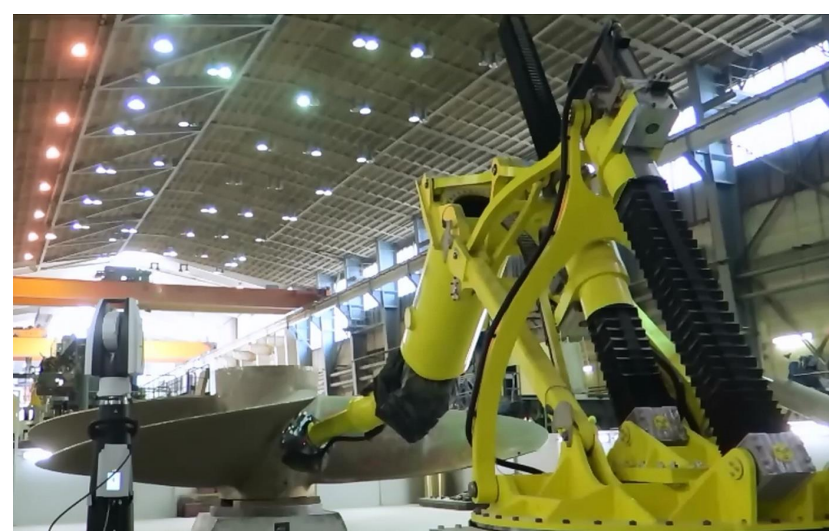
\includegraphics[width=0.6\textwidth]{adaptiveprogramming.png}
  \caption{自适应机器人编程}
  \label{fig:adaptiveprogramming}
\end{figure}
% !TeX root = main.tex
\section{定位与基于位置的服务}

2005年到2014年间，德国的LBS服务提供商数量经历了爆发式增长，年增长率一度非常高。不过这一波增长主要是消费市场驱动的，比如地图导航、社交打卡、外卖跑腿这些面向普通消费者的应用。相比之下，工业生产场景里对LBS的应用还比较有限，目前主要集中在物流环节，比如仓库里货物和叉车的追踪。消费领域已经把这项技术玩得很成熟了，但工业领域还有很大的应用空间没有被打开。

\subsection{原理与方法}

常见的定位原理分为以下几大类。
\begin{enumerate}
    \item \textbf{信号强度法（Signalstärke）}：信号在传播过程中会随距离增大而衰减，只要提前测出一张"信号强度地图"，就能反推出接收点大致在哪里，GSM、UMTS、WLAN、蓝牙定位都属于这个思路，缺点是容易受到障碍物遮挡和信号反射的干扰。
    \item \textbf{飞行时间测量（Laufzeitmessung）}，也就是通过信号传播的时间差来算距离，光速是已知的（大约100皮秒对应3厘米），所以只要测出时间就能算出距离。这里面又细分为\textbf{到达时间法（TOA, Time of Arrival）}、\textbf{到达时间差法（TDOA, Time Difference of Arrival）}和\textbf{往返时间法（RTT, Round Trip Time）}，GPS、伽利略、格洛纳斯这些卫星导航系统用的都是这一类原理。
    \item \textbf{三边测量与三角测量（Triangulation）}，前者是通过测量到多个参照点的距离来确定位置，后者是通过测量角度，立体视觉、光切法、WLAN和蓝牙的一些定位方案会用到这类思路。
    \item \textbf{特征匹配法（Merkmalsbasiert）}：把传感器测到的环境特征（比如激光雷达扫出来的点云）和已有的地图做匹配，比较典型的做法是ICP迭代最近点算法，不过这种方法需要一个比较好的初始猜测值才能收敛。
    \item \textbf{惯性传感法（Intertialsensorik）}：靠加速度计、陀螺仪、地磁传感器等器件，从一个已知的起点开始不断累加位移，缺点是误差会随时间累积，所以实际应用中经常和其他方法组合使用，也就是常说的"混合定位"。
    \item \textbf{相位测量法（Phasenmessung）}：通过测量信号在一个周期内的相位来确定相对或绝对位置，比如利用干扰信号计数脉冲，这种方法精度较高，但通常需要配合其他手段一起使用。
\end{enumerate}
在实际选型时，需要沿着若干维度对候选系统做综合权衡：\textbf{精度（Genauigkeit）}是否满足任务要求；\textbf{作用范围（Arbeitsraum）}能否覆盖目标工作空间；\textbf{基础设施需求（Infrastrukturbedarf）}有多大，是否必须预先布设锚点、反射板或轨道；\textbf{抗干扰能力与鲁棒性（Robustheit）}在存在遮挡、反射和金属结构的车间环境中是否足够；\textbf{可扩展性（Skalierbarkeit）}以及可同时定位的\textbf{目标数量（Teilnehmeranzahl）}能否随产线规模增长；\textbf{可用性（Verfügbarkeit）}，即系统在多大比例的时间和空间内能给出有效位置；所用\textbf{频段（Frequenzen）}是否合规、是否与厂内既有无线系统冲突；\textbf{成本（Kosten）}，包括设备、安装与运维；\textbf{信息安全（Security）}；以及该技术的\textbf{市场成熟度（Marktbedeutung）}与供应商生态。图  直观地展示了各种室内定位技术在精度和作用范围这两个维度上的分布，从毫米级的摄像头、超宽带（UWB）定位，到覆盖整栋建筑的WLAN和蜂窝网络定位。

\begin{figure}[htbp]
  \centering
  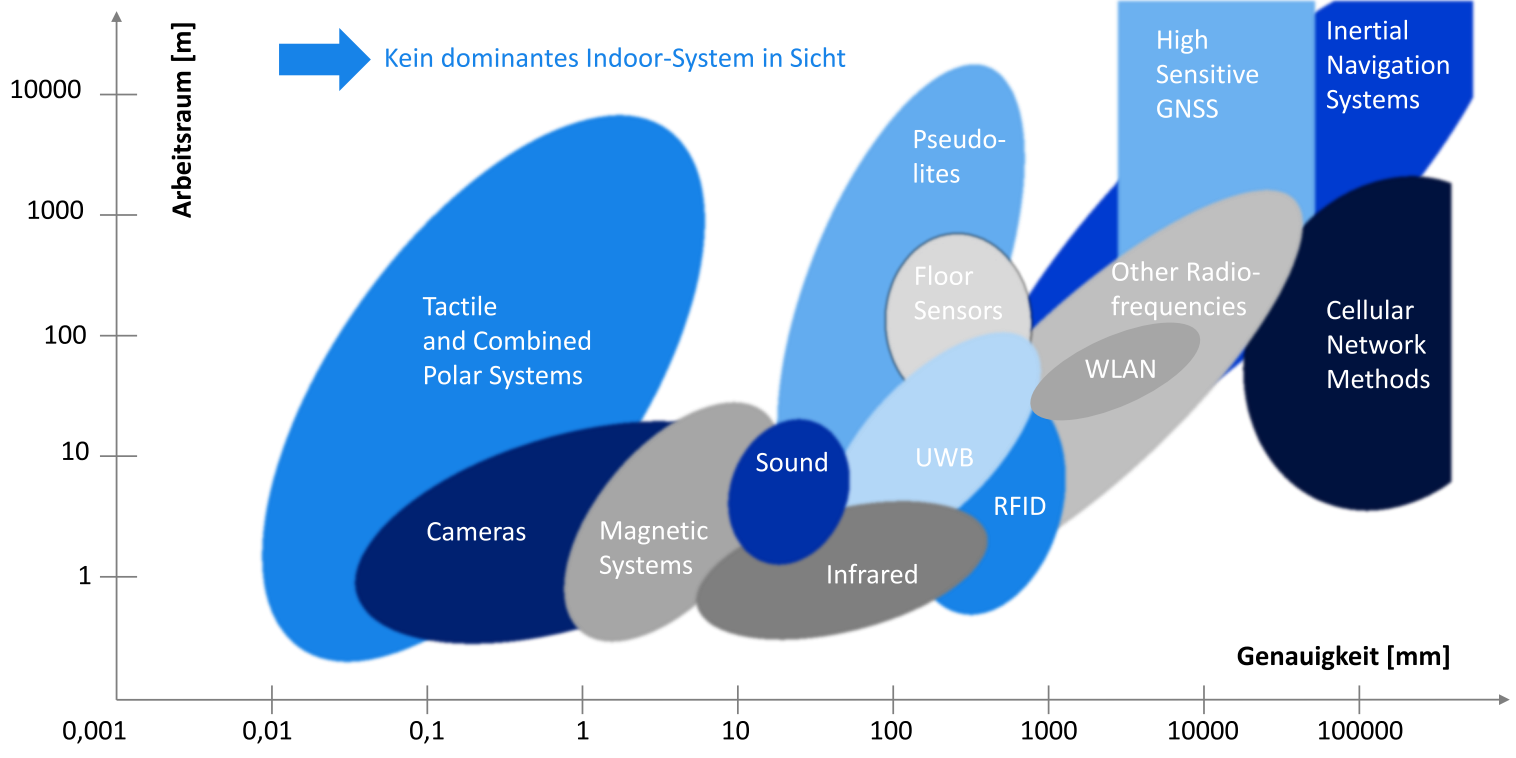
\includegraphics[width=0.7\textwidth]{indoorlokalisierungverteilung.png}
  \caption{各种室内定位技术在精度和作用范围这两个维度上的分布}
  \label{fig:indoorlokalisierungverteilung}
\end{figure}

目前室内定位领域还没有出现像GPS在室外那样一统天下的主流方案，这也是这个领域仍然活跃、值得研究的原因之一。

\subsection{地图}

有了定位能力之后，接下来要解决的问题是这些位置信息怎么组织和呈现，也就是地图。例如我现在要找到最近的服装店或餐厅，并从我当前位置导航过去，这个简单需求背后其实包含了四层能力：把信息画出来给人看（图形化展示）、按条件搜索兴趣点（POI搜索）、规划一条路线、以及实时导航。

地图本质上是数据，只是被组织成了人类容易理解的形式。不同的应用场景需要不同的数据结构来支撑，课程介绍了室内环境建模的四种典型思路。
\begin{enumerate}
    \item \textbf{基于网格的几何建模（Cell based）}，也叫占据栅格地图，把空间切成一个个小格子，每个格子标记是否被占用。
    \item \textbf{基于边界的几何建模（Boundary Based）}，用轮廓线来描述空间和物体的边界。
    \item \textbf{基于符号或地点的建模（Symbolic/Place based）}，不追求精确的几何形状，而是用"房间""通道"这类语义化的地点概念来组织空间。
    \item \textbf{混合式建模（Hybrid）}，把面向对象的方法和边界建模结合起来，兼顾精确性和语义信息。
\end{enumerate}
这几种方式各有取舍，选哪一种取决于具体应用对精度、灵活性和计算成本的要求。



\subsection{基于位置的服务}

有了定位能力和地图这两块基础之后，就可以在其上构建各类基于位置的服务（LBS）。汇总出以下十种类型：
\begin{enumerate}
  \item \textbf{参照定位（Referenzierung）}：为后续一切位置信息提供一个基准，即把对象的位置表达为相对于某个已知参考系或参考点的相对位置，本身不关心姿态。
  \item \textbf{定位（Positionierung）}：在参照的基础上确定对象的实际位置，通常不只给出位置，还包括姿态，即完整的位姿（Pose）；这是与参照定位的主要区别。
  \item \textbf{导航（Navigation）}：在已知自身位姿和环境模型的前提下，给出应当行驶的路径或轨迹，并在行驶过程中持续跟踪与修正，是移动机器人和搬运车辆的核心服务。
  \item \textbf{质量保证（Qualitätssicherung）}：借助位置信息保证工序在正确的位置、按正确的顺序执行，重点在于避免错误的产生，而不是事后把错误检出来，例如拧紧工具只有在正确的螺栓位置上才被使能。
  \item \textbf{文档记录（Dokumentation）}：对位置信息做持续的追踪和留痕，往往是出于法规或合规要求（如可追溯性、责任认定），记录本身即是目的。
  \item \textbf{数据分析（Analyse）}：在文档记录所积累的位置数据之上做进一步的评估，比如识别搬运路径中的绕行与瓶颈、统计设备利用率，用于流程优化；与文档记录的区别在于目的是分析而非留证。
  \item \textbf{信息提供（Information）}：依据使用者当前所处的位置提供相应的信息，比如给工人推送与他当前工位、当前任务相关的作业指导，这也是增强现实（AR）应用的基础。
  \item \textbf{安全防护（Safety）}：防止人员受到设备的伤害，比如人员接近危险区域时自动预警、降速或停机。
  \item \textbf{防范恶意行为（Security）}：也包括厂区与资产的防护，识别人或设备的异常行为并采取应对措施；由于两者在技术手段上高度重叠，Security 与 Safety 之间的界限在实践中并不容易划清。
  \item \textbf{绩效管控（Leistungssteuerung）}：借助位置数据确定所需的绩效参数（如节拍、行程、等待时间），并在必要时对人员或设备的工作表现加以调控。
\end{enumerate}

值得一提的是，定位技术在工业场景中的应用是具有许多风险和限制的，尤其是当定位信息被用来监控员工的行为和绩效时。比如键盘输入速度监测、通话记录、屏幕操作追踪，这些技术手段虽然可行，但会直接触及员工的人格权和隐私权，在德国的实际操作中，这类系统的引入和使用受到《联邦数据保护法》的约束，并且必须经过企业职工委员会的共同决策程序，不能由企业单方面决定。

真实案例：运动软件Strava发布的全球运动热力图，因为记录了大量军人在军事基地内跑步的轨迹，无意中暴露了一些本应保密的军事设施位置和内部路网布局，这个例子很直观地说明了定位数据一旦被聚合和分析，可能带来意想不到的信息泄露风险。这提醒我们，定位技术在带来便利的同时，也需要认真考虑数据安全和个人隐私的边界。

\paragraph{示例：厂内物流中的定位应用}

在如图  所示的这样一个工厂中，有许多自动搬运机器人，它们要完成货物的取放和运输任务，需要具备几项核心能力：
\begin{enumerate}
  \item \textbf{任务规划（Handlungsplanung）}：把一个大任务拆解成一步步可执行的动作
  \item \textbf{导航（Navigation）}：包括自身定位、路径规划和路径跟踪
  \item \textbf{避障（Kollisionsvermeidung）}：绕开障碍物、识别危险情况
  \item \textbf{物体识别（Objekterkennung）}：认出托盘、行人、其他车辆
  \item \textbf{交通调度（Verkehrsregelung）}：多台机器人之间的优先级协调和死锁避免
\end{enumerate}

\begin{figure}[htbp]
  \centering
  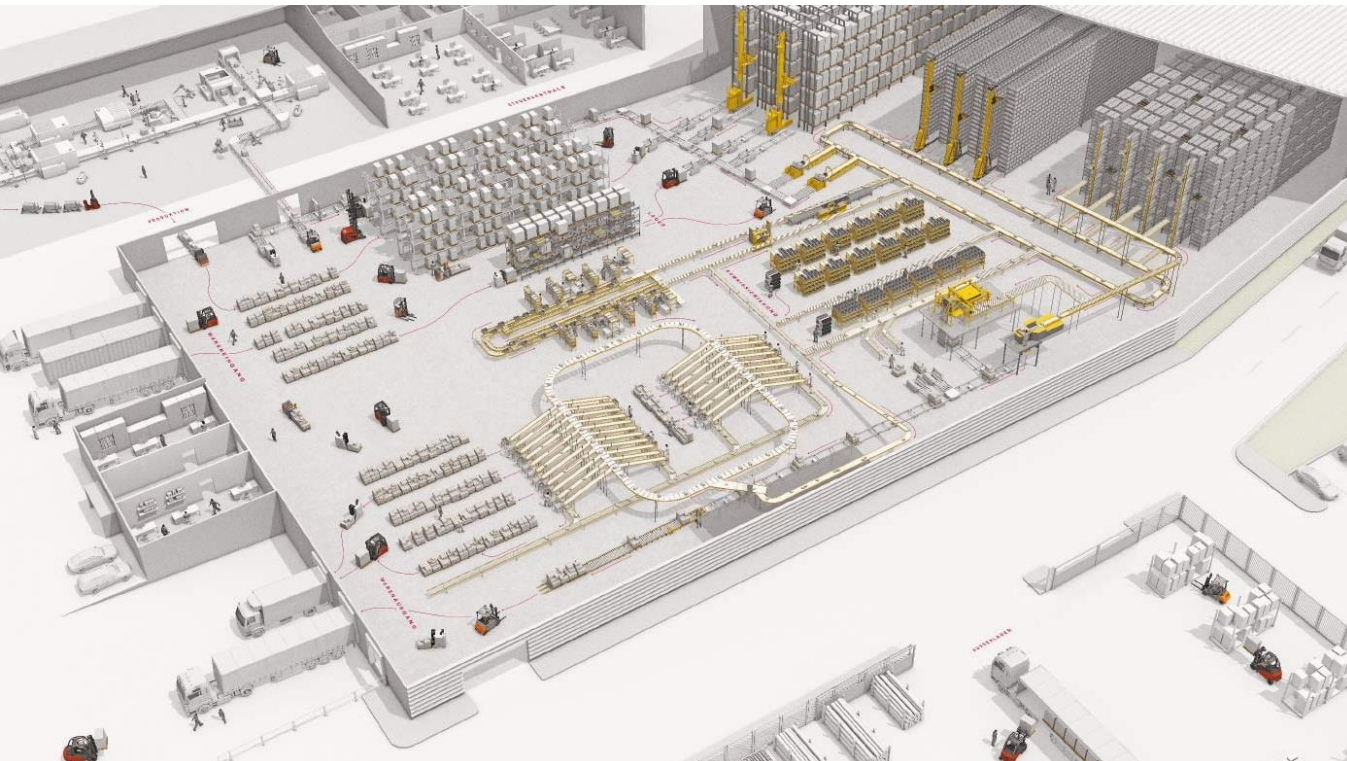
\includegraphics[width=0.7\textwidth]{intralogistik.png}
  \caption{需要许多自动搬运机器人的工厂}
  \label{fig:intralogistik}
\end{figure}

导航环节里的自身定位，对比了几种在物流仓库里常见的定位方案：光学或电磁轨道引导（车辆沿着地面铺设的轨迹行驶）、磁点导航（依靠预埋在地面的磁性标记点）、二维激光反射板定位（依靠悬挂在环境中的反射板作为参照）、以及基于自然地标的定位（不需要额外布置标记物，直接利用环境本身的特征，又分为二维和三维两种做法）。这几种方案在地图生成的难易程度、定位精度、对生产流程调整的适应能力、以及安装部署的成本上各有优劣。

\paragraph{示例：航空维修行业的实际项目}

第二个案例来自航空维修领域，讲的是汉莎技术公司（Lufthansa Technik）的"GSE 4.0"项目。GSE指的是机场地面保障设备（Ground Support Equipment），如图 \ref{fig:gse40} 所示，汉堡基地目前有超过1500台这样的设备在使用，而一架飞机在地面停留维修期间，大约需要用到500台GSE。

\begin{figure}[htbp]
  \centering
  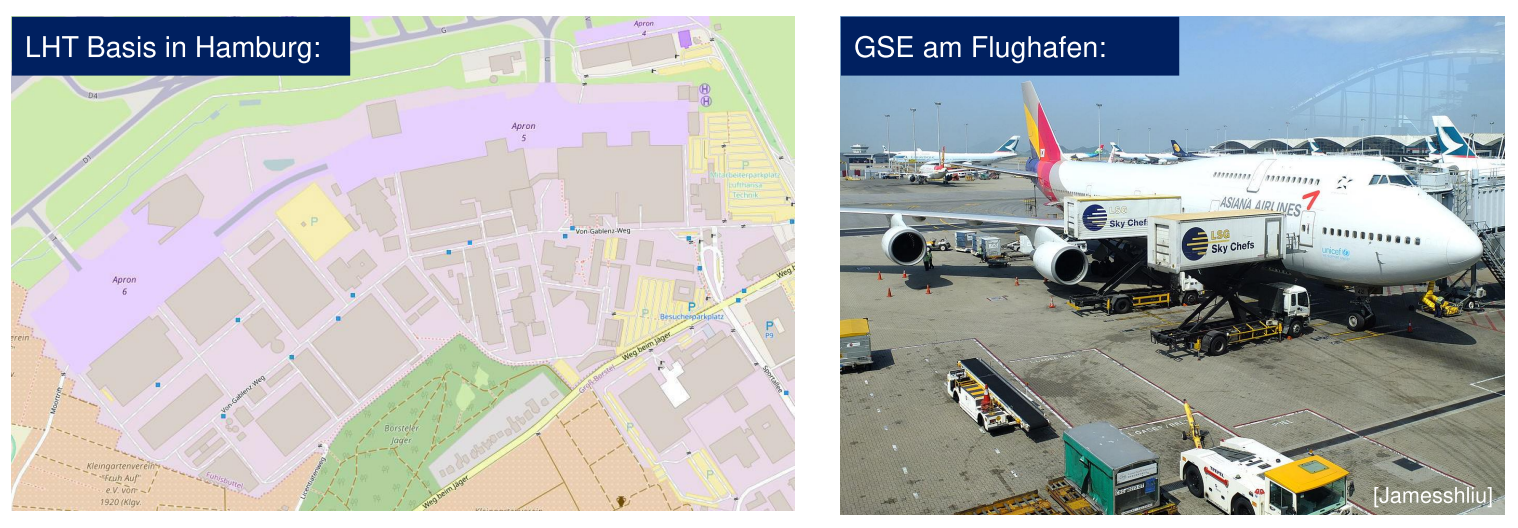
\includegraphics[width=0.9\textwidth]{gse40.png}
  \caption{Lufthansa Technik 的 GSE 4.0 项目}
  \label{fig:gse40}
\end{figure}

这个项目要解决的问题很实际：设备使用完之后经常被随手放在没有固定规划的地方，下一个需要用它的机修工人就得花时间到处寻找，白白浪费了工时，也没法把设备的利用率提到最高。项目的解决思路是给每台设备装上定位标签，让设备之间通过蓝牙（BLE）互相定位，具体的定位方式是基于信号强度（RSS）；同时在建筑物上安装若干锚点标签作为本地定位的参照物；设备的标签在设定的事件触发时把自己的位置信息发送给LoRa网关（这种网关的信号覆盖范围可以达到几公里）；网关再通过移动网络把位置数据统一传回中心数据库。有了这套基础设施之后，就可以在此之上搭建出好几种实用的LBS功能：设备的实时追踪和状态查询、按需的临时预约申请、以及提前的使用计划安排。最终效果是让设备管理从原来分散、被动的状态，变成\textbf{集中协调、可以提前规划的状态，明显提高了透明度，也减少了设备闲置或找不到的时间}。

\paragraph{工业室内定位}

IFPT研究所正在做的科研项目 IIL（Industrielle Indoor Lokalisierung）。

矩阵图 \ref{fig:iil} 说明了这个项目的出发点：生产制造过程中的不同环节，比如寻找物料、搬运、抓取、组装、加工、检测——对定位精度的要求差异非常大，从米级（找东西大概知道在哪个区域就够了）一直到微米级（比如精密测量环节），这些不同层级的需求分别对应着信号强度、飞行时间、三边测量、三角测量等不同的技术手段，没有一种定位技术能够单独覆盖所有场景。

\begin{figure}[htbp]
  \centering
  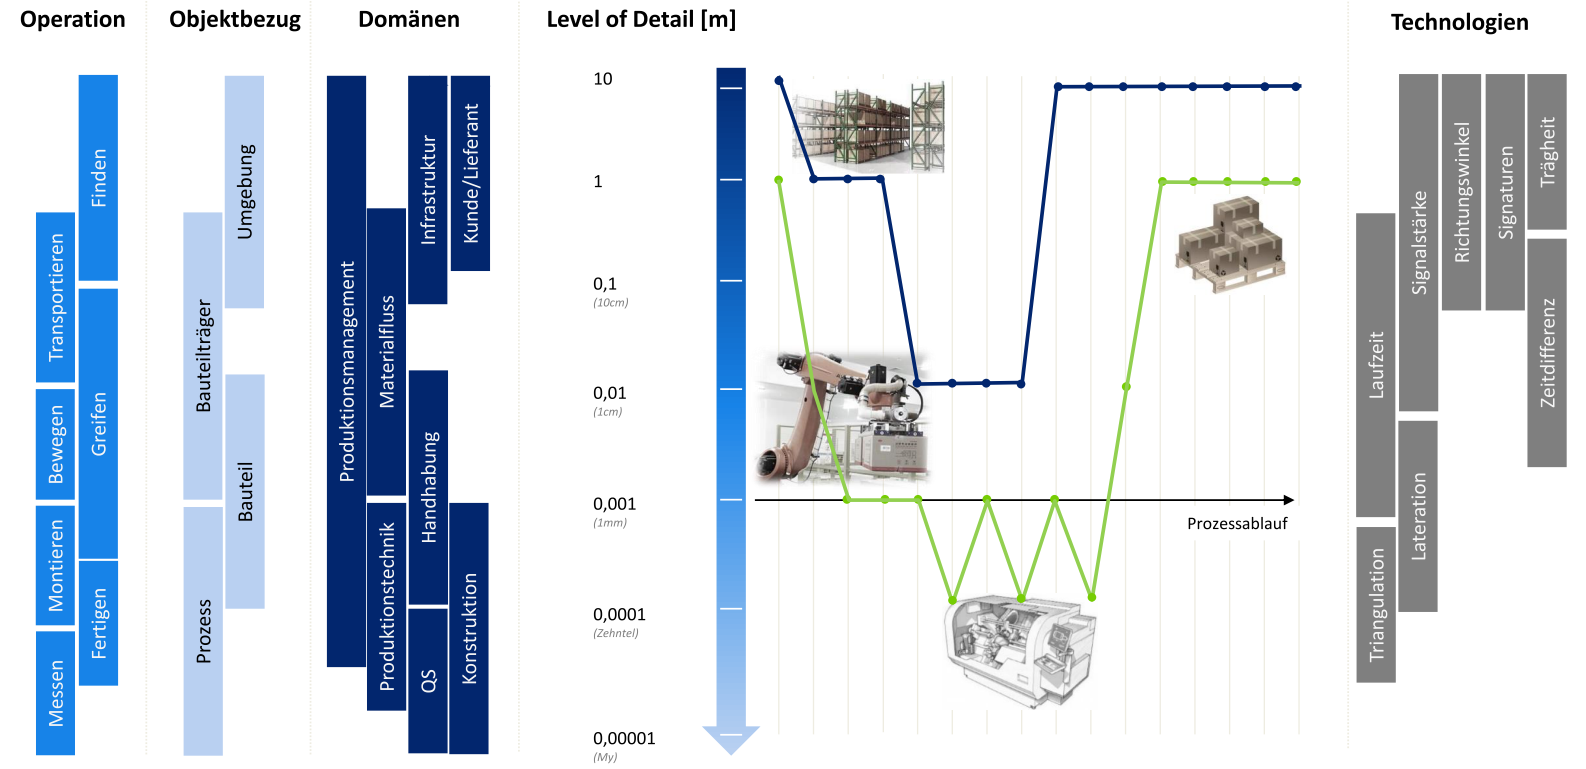
\includegraphics[width=0.9\textwidth]{iil.png}
  \caption{生产制造过程中不同层级的需求}
  \label{fig:iil}
\end{figure}

用大家都很熟悉的谷歌地图做类比，一个好的环境模型应该是分层和可集成的：卫星图像有不同精细程度的层级，再叠加街景图、社区标注、路况信息、矢量数据等，这些不同来源、不同类型的数据整合在一起，才构成了我们平时用起来很顺手的地图产品。IIL项目想做的，就是把工厂里各种来源的定位信息（比如移动机器人的定位、增强现实设备的定位、智能工具的定位、移动测量设备的定位）也用类似的思路整合起来，形成一个统一的位置信息底座，再向上支撑数字工厂、LBS等各类应用。
% !TeX root = main.tex
\section{工业数据科学}

\subsection{简介}

理解数据分析能做到什么程度，常用一条从低到高的价值线：
\begin{enumerate}
    \item 描述性分析（Descriptive）：回答发生了什么，是最基础的观察和统计
    \item 诊断性分析（Diagnostic）：回答为什么会发生，需要解释原因
    \item 预测性分析（Predictive）：回答接下来会发生什么，需要对未来做预判
    \item 规范性分析（Prescriptive）：回答应该怎么做，直接给出行动建议
\end{enumerate}
越高的等级能带来的业务价值越大，技术难度也越高。描述这类海量、复杂数据的特征，通常用\textbf{3V}：
\begin{itemize}
    \item Volume（容量）
    \item Velocity（速度）
    \item Variety（多样性）
\end{itemize}


\subsection{CRISP-DM}

接下来我们用 \textbf{CRISP-DM（Cross-Industry Standard Process for Data Mining，跨行业数据挖掘标准流程）}来讲解一个喷油器的案例。这套方法论把一个完整的数据科学项目拆成六个阶段：
\begin{enumerate}
    \item \textbf{业务理解（Business Understanding）}：搞清楚项目到底要解决什么问题
    \item \textbf{数据理解（Data Understanding）}：搞清楚手头有什么数据、质量如何
    \item \textbf{数据准备（Data Preparation）}：把原始数据加工成能喂给模型的形式
    \item \textbf{建模（Modeling）}：选择合适的算法，训练模型
    \item \textbf{评估（Evaluation）}：判断模型到底好不好用
    \item \textbf{部署（Deployment）}：把模型真正用到实际生产决策中去
\end{enumerate}
这六个阶段不是一次性走完就结束的直线流程，而是一个可以循环迭代的闭环。评估阶段发现问题，往往要回头重新做数据准备甚至业务理解。

喷油器的生产分为部件加工和总装两大部分。总装线上要经历一连串工序，最后要经过一套完整的液压终检。这是一种 100\% 全检，每个产品要在多个检测点（P1、P2……）上分别测量喷射量、压力、回流量等多项特性，再和规格比对，最终打上合格标签。问题在于这种全检非常耗时，成了整条生产线的瓶颈工序。项目要解决的目标很明确：通过数据分析提前预测最终检测点的结果，从而减轻检测环节的压力。

拿到原始数据后往往不能直接拿去训练模型，通常要先完成几件事：
\begin{itemize}
    \item 数据清洗：识别并处理不可用的数值。
    \item 数据变换：不同的数据往往处在不同的量纲层级上。需要做升级或降级处理，让不同类型的数据能放在一起比较。
    \item 特征提取：每个检测点采集到的原始曲线通过特征提取转换成模型可以使用的特征。
\end{itemize}

数据准备好之后，就进入建模阶段。训练模型可以有多种机器学习的方法，例如线性回归、逻辑回归、k近邻、支持向量机等等，这些机器学习的方法会在第\ref{sec:aiml}章节中详细介绍。模型训练完了，还需要一套指标来判断它靠不靠谱。标准做法是用\textbf{混淆矩阵}框架，把预测结果和真实结果交叉对比，划分出四种情况：
\begin{itemize}
    \item \textbf{阳性（TP）}：预测不合格，实际也确实不合格
    \item \textbf{假阳性（Pseudofehlerrate, FP）}：预测不合格，但实际是合格的，伪错误。意味着模型"多疑"，把好产品误判成了坏产品
    \item \textbf{假阴性（Schlupfrate, FN）}：预测合格，但实际是不合格的，这类错误被称为漏检，是更危险的一种错误，意味着有缺陷产品被放过去了
    \item \textbf{真阴性（TN）}：预测合格，实际也确实合格
\end{itemize}
在这四个数字的基础上，可以算出一整套评估指标：
\begin{itemize}
    \item\textbf{精确率（Precision）}衡量被预测为合格的产品里，有多少是真的合格
    \item \textbf{召回率（Recall）}衡量所有真正不合格的产品里，有多少被成功抓出来了
    \item \textbf{特异度（Specificity）}衡量所有真正合格的产品里，有多少被正确放行了
    \item \textbf{准确率（Accuracy）}则是预测正确的比例，也就是 (TP+TN) / 全部样本数
    \item \textbf{伪错误率}：FP 占比
    \item \textbf{漏检率}：FN 占比
\end{itemize}
喷油器数据上跑出的结果整体准确率达到 96.15\%，但召回率只有 33.83\%，也就是说，虽然总体判断准确，但真正能抓出来的不合格品其实只占三分之一左右。这说明单看准确率会掩盖问题，必须结合多个指标一起看。

漏检率和伪错误率之间存在此消彼长的权衡。想把漏检率压得更低，往往就得接受更高的伪错误率，反之亦然。选哪个模型、定在哪个平衡点，最终要看业务上更能承受哪种代价。


\section{人工智能与机器学习}

\subsection{制造业里的 AI 与 ML}

理解机器学习之前，有必要先区分两个常被混用的概念。强人工智能主张 AI 系统可以具备和人类相同、甚至超越人类的智力能力；弱人工智能则聚焦于用数学和信息学方法解决具体的应用问题，系统具备一定的自我优化能力，过程中会模拟人类智能的某些方面，或者构建用于模拟、辅助人类思考的系统。目前工业界能落地的绝大多数应用，属于弱人工智能的范畴。

而机器学习的核心机制是：机器从已有的样本数据中识别模式，据此构建模型，再把学到的知识应用到此前未见过的新情况上。数据量越大、信息越丰富，模型学到的效果通常越好。

生产领域被认为是机器学习应用潜力最大的场景之一，服务、客户服务和物流等领域同样存在丰富的应用空间。机器学习在系统自我优化与自我适应方面展现出很强的潜力。

几个因素正在加速机器学习技术在工业场景中的落地：开发环境的显著进步降低了使用门槛；特征工程这一原本繁琐的环节被大大简化；性能优异的预训练网络结构（尤其在图像分析与识别领域）可以直接复用；专用且成本更低的硬件也加快了模型训练的速度。这几个使能因素共同解释了为什么近年来机器学习方法能够更快地走出实验室、进入实际产线。

\subsection{图像特征}

机器视觉要解决的根本问题可以归结为两个问题：人类究竟依据哪些信息（图像特征）在视觉上识别出物体？这些信息又该如何表示，才能让计算机也具备识别物体的能力？

从算法角度看，这个问题可以进一步拆成两个子任务。分类任务是把一次观测分配给某个类别；而机器学习的任务则是学习出一组类别边界，使这种分配尽可能不出错。

对图像特征本身，有三点基本要求：可靠性（同一物体在不同条件下能被稳定识别）、可计算性（提取特征所需的计算开销要可控）、可区分性（不同类别的特征要能被明确区分开）。图像特征大致可以分成两类：一类是特定的强度变化（亮度变化），可以通过梯度大小、梯度方向、卷积操作（滤波器）等方式量化计算；另一类是图像局部区域内强度变化在特定方向上的分布，常用方向直方图来描述。

在卷积神经网络普及之前，图像特征提取主要依赖两条技术路线：基于梯度的方法，以及基于统计分布的方法。

\paragraph{基于梯度的方法}

Moravec 角点检测器是较早的思路：取图像中一个小窗口，把这个窗口分别向不同方向做微小平移，观察平均亮度的变化情况——几乎没有变化说明处在平坦区域；只在特定方向平移时亮度发生明显变化说明处在边缘上；无论向哪个方向平移亮度都明显变化则说明处在角点上。这种方法的缺点是滤波响应具有各向异性，而且二值化的矩形窗口容易受噪声干扰。

Harris 角点检测器针对这个问题做了改进：通过每个像素点处灰度函数的偏导数构建一个结构矩阵，矩阵的特征值反映边缘强度，特征向量反映边缘方向，特征值可以通过矩阵的迹和行列式求出。这样得到的滤波响应具有各向同性，对平移和旋转具有不变性，对亮度变化也有一定的鲁棒性，但缺点是不具备尺度不变性。

Haar 特征最初是为人脸检测设计的，思路来自 Haar 小波（与傅里叶分析类似）：对图像区域内的强度做乘法和求和运算，强度相近时得到较低的数值，强度差异大时得到较高的正负数值；借助积分图技术可以高效计算像素求和，大幅提升计算速度。

\paragraph{基于统计分布的方法}

方向梯度直方图（Histogram of Oriented Gradients，HOG）先做预处理，再对每个像素通过卷积运算计算梯度的大小和方向；接着把图像窗口划分成若干局部单元格，每个单元格内的梯度汇总成一个方向直方图；最后对重叠的区块做归一化处理。HOG 的优点是得到的特征向量可以直接作为分类器的输入，且计算速度快、特征表达能力强；缺点是需要预先设定固定的窗口尺寸，对旋转、尺度和平移变化的鲁棒性有限。

尺度不变特征变换（Scale Invariant Feature Transform，SIFT）则是为了解决尺度和旋转不变性的问题：它能找到图像中的关键点（Keypoints）并用特征向量描述，这种描述对尺度和旋转具有不变性，同时对仿射畸变、视角变化、噪声和光照变化都有较好的鲁棒性。SIFT 算法大致分四步：先在尺度空间中确定候选关键点，尺度空间的构建依赖对同一图像做不同程度的高斯模糊，再把相邻模糊程度的图像相减（高斯差分），这是一种能快速突出边缘、生成梯度图像的方法；接着筛选和定位关键点；再为每个关键点分配一个主方向，把邻域按主方向旋转以获得旋转不变性；最后用邻域内的方向直方图描述每个关键点，得到一个 128 维的特征向量。

\subsection{卷积神经网络}

经典方法有一个共同的痛点：特征提取环节高度依赖人工设计和专家经验，需要反复尝试和评估不同的特征提取与分类方案，费时费力。卷积神经网络（CNN）最大的价值就在于取消了这道特征工程的门槛。特征提取被整合进分类模型内部，训练过程中自动完成，这种从原始图像直接到分类结果的方式被称为端到端学习（End-to-End Learning）。

如图 \ref{fig:cnn} 所示：CNN 的核心组件是卷积层：神经元按宽度、高度、深度三个维度排列，专门为图像处理设计。卷积层的参数由一组可学习的感受野滤波器（权重矩阵）组成，这些滤波器也被称为特征检测器，其宽高通常远小于输入图像，滤波器的数量对应输入图像的深度。在每个位置上，滤波器的各个通道与图像对应区域的通道逐元素相乘再求和，这个操作就是卷积；一个滤波器在整张图像上卷积得到的结果构成一张特征图（Feature Map），特征图中被突出显示的区域，就是与该滤波器最相似的区域。

\begin{figure}[htbp]
  \centering
  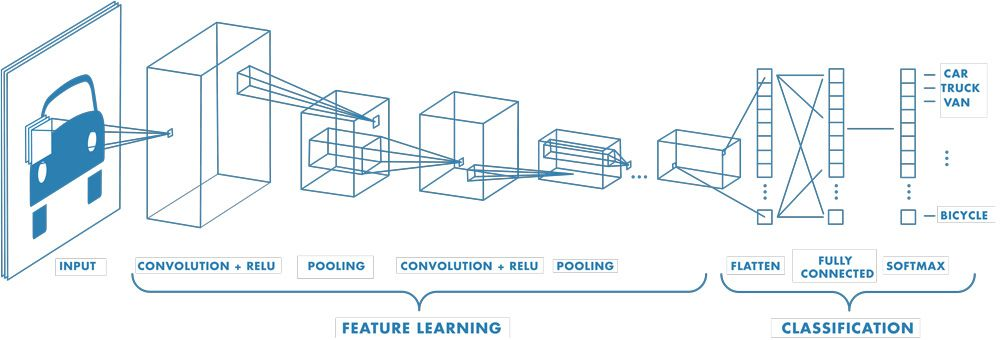
\includegraphics[width=0.8\textwidth]{cnn.jpg}
  \caption{卷积神经网络}
  \label{fig:cnn}
\end{figure}

池化层通常夹在两个卷积层之间，作用是从前一卷积层得到的特征图中剔除对模式识别而言冗余的参数，从而降低计算量。通过多层卷积和池化的堆叠，网络可以构建出复杂的非线性映射关系：层与层之间形成一种层级结构，逐步实现自动特征提取，特征也随层数加深逐级浓缩。每个节点基于前一层的输出学习特定的特征——最初的几层通常只识别角点、边缘等简单模式，越往后的层则负责聚合和组合这些简单模式，从而识别出更复杂的形状和物体。

\subsection{图像内容分类}

经典分类方法中，贝叶斯分类器基于贝叶斯定理
\begin{equation}
    P(c|x) = \frac{P(x|c)\cdot P(c)}{P(x)}
\end{equation}
对给定的观测 \(x\)，选择使后验概率 \(P(c|x)\) 最大的类别作为判断结果。它的优点是模型简单、易于实现，且所需的训练数据量较少。

k 近邻（k-Nearest-Neighbor）走的是一条更直观的路线，如图 \ref{fig:knn} 所示：判断一个未知物体属于哪一类，依据是它和已知物体之间的相似度，相似度通过距离度量转换成具体数值来表达。优点是分类器直观、实现简单，同时又能够拟合比较复杂的类别边界。

\begin{figure}[htbp]
  \centering
  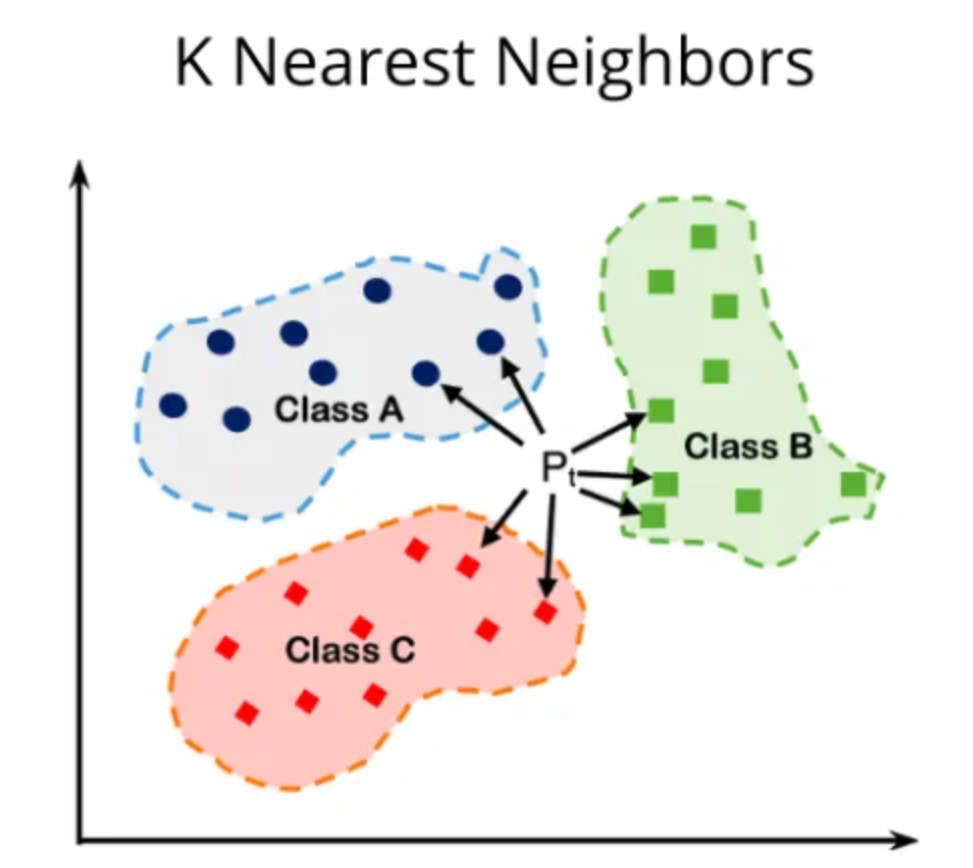
\includegraphics[width=0.4\textwidth]{knn.png}
  \caption{k 近邻分类器}
  \label{fig:knn}
\end{figure}

如图 \ref{fig:svm} 所示，支持向量机（SVM）的核心思路是用一个超平面把线性可分的数据分开，并让训练样本（支持向量）到分界面的正交距离尽可能大；对于线性不可分的数据，可以通过映射到更高维的特征空间来处理，这就是常说的核技巧（Kernel-Trick）。

\begin{figure}[htbp]
  \centering
  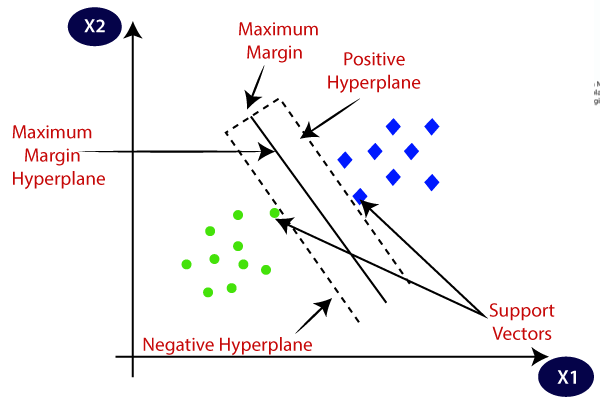
\includegraphics[width=0.4\textwidth]{svm.png}
  \caption{支持向量机}
  \label{fig:svm}
\end{figure}

神经网络的基本结构是：输入值通常写成向量 \(x=(x_1, x_2, \ldots, x_m)\)，每个输入对应一个网络权重 \(w_i\)，网络活性 net 由输入与权重的加权和计算得出，再经过一个激活函数 \(f(x)\) 得到输出。可以调节的超参数包括网络架构或拓扑结构（神经元数量、层数、连接方式）、激活函数的类型（阈值函数、Sigmoid 函数等）、训练过程中权重的调整方式（反向传播算法），以及阈值的调整方式。

用CNN做分类时，网络末端通常接若干全连接层（Fully Connected Layers，FC）。倒数第二个全连接层输出一个长度为 \(k\) 的向量，\(k\) 等于类别数量；对这一层应用 Softmax 激活函数，计算出每个类别对应的概率，所有类别的概率加起来正好等于 1。

\end{document}
